\RequirePackage[l2tabu, orthodox]{nag} %编译时,给出过时命令和不规范使用警告。

\documentclass[UTF8, fontset = none, a4paper, twoside, openany, zihao = -4,
scheme=chinese, no-math]{ctexbook}

\setCJKmainfont
[
  BoldFont = SourceHanSerifCN-Bold.otf ,
  ItalicFont = FZXKTJ.otf
] {SourceHanSerifCN-Regular.otf}
\setCJKsansfont
[
  BoldFont = SourceHanSansCN-Medium.otf
] {SourceHanSansCN-Normal.otf}
\setCJKmonofont {FZFSJ.otf}
\setCJKfamilyfont { zhsong }
[
  BoldFont = SourceHanSerifCN-Bold.otf
] {SourceHanSerifCN-Regular.otf}
\setCJKfamilyfont { zhhei }
[
  BoldFont = SourceHanSansCN-Medium.otf
] {SourceHanSansCN-Normal.otf}
\setCJKfamilyfont { zhfs } {FZFSJ.otf}
\setCJKfamilyfont { zhkai }
[
  BoldFont = FZCKJW.ttf
] {FZXKTJ.otf}

\NewDocumentCommand \songti   { } { \CJKfamily { zhsong } }
\NewDocumentCommand \heiti    { } { \CJKfamily { zhhei } }
\NewDocumentCommand \fangsong { } { \CJKfamily { zhfs } }
\NewDocumentCommand \kaishu   { } { \CJKfamily { zhkai } }

\global\hyphenpenalty=5000
\global\tolerance=1000

\usepackage{amsmath, amssymb, xfrac}
\usepackage[math-style=ISO, bold-style=ISO]{unicode-math} %注意,unicode-math与被其认为过时的bm包不兼容,不要\usepackage{bm}
\setmainfont[Scale=1.1, SlantedFont = libertinusserif-italic.otf, BoldFont = libertinusserif-bold.otf]{libertinusserif-regular.otf}
\setmathfont[AutoFakeBold,Scale = 1.15]{libertinusmath-regular.otf}  % 因Libertinus目前的数学字体暂还没

\setsansfont{TeX Gyre Heros}
\defaultfontfeatures{Scale=MatchLowercase}

\usepackage[backend=biber,style=gb7714-2015,backref=true]{biblatex}
\addbibresource[location=local]{ref/refs.bib}
\renewcommand{\bibfont}{\zihao{5}}
\renewcommand{\bibauthorfont}{\bfseries\color{teal}}%
\renewcommand{\bibtitlefont}{\itshape\color{blue}}%
\renewcommand{\bibpubfont}{\rmfamily\color{violet}}%
\def\UrlFont{\ttfamily}

\usepackage{verse}

\ctexset{%
  abstractname = {摘\quad 要},  % book类没有摘要
  bibname = {参考文献},
  today = {big},
  subsection/format += \centering
}


% 插图所需的宏包
\usepackage{graphicx}
\graphicspath{{figures/}}

\usepackage{caption}
\captionsetup{font=small, labelfont=bf}



\usepackage{etoolbox}
\newcommand{\capsource}[1]{\vspace{-8pt} \caption*{\mdseries 图表来源: {#1}} } % 自定义图表来源
                                % 命令,vspace可酌情调整。
% % 脚注按页编号

\usepackage{pifont}
\let\oldding\ding% Store old \ding in \oldding
\renewcommand{\ding}[2][1]{\scalebox{#1}{\oldding{#2}}}% Scale \oldding via optional argument

\usepackage[perpage, hang, symbol*]{footmisc}
\DefineFNsymbols{cqufnsymbol}{
    {\ding[1.3]{172}}    {\ding[1.3]{173}}
    {\ding[1.3]{174}}    {\ding[1.3]{175}}
    {\ding[1.3]{176}}    {\ding[1.3]{177}}
    {\ding[1.3]{178}}    {\ding[1.3]{179}}
    {\ding[1.3]{180}}    {\ding[1.3]{181}}
}
% 定义footnote的表示方法为cqufnsymbol
\setfnsymbol{cqufnsymbol}
% minipage需要额外定义一行
\renewcommand\thempfootnote{\fnsymbol{mpfootnote}}

\usepackage{scrextend}
\deffootnote{0em}{1.6em}{\thefootnotemark\enskip}

\AtBeginEnvironment{quotation}{\kaishu}


\usepackage{fancyhdr, geometry}

\geometry{%
  a4paper,
  heightrounded,
  includemp = true, % includes the margin notes, \marginparwidth and \marginparsep, into body when calculating horizontal calculation.
  marginparsep = 0.3cm,
  marginparwidth = 2.5cm,
  top = 3cm,
  bottom = 3cm,
  % left = 2.6cm,
  % right = 2.6cm, % 如果要为todonotes包要使用的 marginparwidth 留出空间的话,尽量
  %                % 将其改小,如0.5cm
  outer = 0.5cm, % twopage 应当使用inner,outer,而不是left,right
  inner = 2.6cm,
  headheight = 6mm,
  headsep = 5mm,
  footskip = 10mm,
}

\usepackage{emptypage} %空白页没有页眉页脚
% \pagestyle{headings}
% \fancyhf{} % clear all header and footer fields
% \lhead{}
% \rhead{}
% \chead{\slshape \zihao{5} \leftmark}
\pagestyle{fancy}

\fancyhf{} % clear all header and footer fields
\fancyhead[LE,RO]{\slshape \zihao{5} \thepage}
\fancyhead[RE]{\slshape \zihao{5} \leftmark}
\fancyhead[LO]{\slshape \zihao{5} \rightmark}
\renewcommand{\headrulewidth}{0.75pt}
\renewcommand{\footrulewidth}{0pt}
\fancyheadoffset{0cm}
\setlength\parskip{0em plus 4pt minus 2pt}

\ctexset{
  part/pagestyle = empty,
	chapter = {
		pagestyle = empty, beforeskip = {-30pt}, afterskip = {20pt plus 5pt}},
  section =
  {beforeskip = {3ex plus 1ex minus 0.2ex}, afterskip = {2.3ex plus 0.2ex}},
	subsection =
  {beforeskip = {3ex plus 1ex minus 0.2ex}, afterskip = {1.5ex plus 0.2ex}},
	subsubsection =
  {beforeskip = {3ex plus 1ex minus 0.2ex}, afterskip = {1.5ex plus 0.2ex}}
}

% from package hyperref
\usepackage{hyperref}
\hypersetup{%
  colorlinks = true,
  citecolor=magenta,
  linkcolor=blue,
  bookmarksnumbered = true,
  pdftitle = {丁家庄},
  pdfcreator = {sd44sd44@yeah.net},
  pdfauthor = {蛋疼的蛋蛋},
  % pdfsubject = {丁家庄城中村},
  % pdfkeywords = {丁家庄, 城中村, 新型城镇化, 社会空间, 社会排斥}
}

\usepackage{microtype} % 改善单词、字母间距
\usepackage{cleveref}

\crefname{equation}{公式}{公式}
\crefname{table}{表}{表}
\crefname{figure}{图}{图}
\crefformat{equation}{#2式~\textnormal{(}#1\textnormal{)}~#3}
\crefformat{figure}{#2图~#1~#3}
\crefformat{table}{#2表~#1~#3}
\crefformat{listing}{#2清单~#1~#3}
\crefformat{page}{#2第~#1~页#3}
\crefformat{line}{#2第~#1~行#3}
\crefformat{part}{#2第~#1~部#3}
\crefformat{chapter}{#2第~#1~章#3}
\crefformat{section}{#2~#1~节#3}
\crefformat{subsection}{#2~#1~节#3}
\crefformat{appendix}{#2附录~#1~#3}
\crefformat{enumi}{#2第~#1~点#3}
\crefformat{footnote}{#2脚注~#1~#3}
\crefformat{definition}{#2定义~#1~#3}
\crefformat{notation}{#2记号~#1~#3}
\crefformat{theorem}{#2定理~#1~#3}
\crefformat{lemma}{#2引理~#1~#3}
\crefformat{corollary}{#2推论~#1~#3}
\crefformat{proposition}{#2命题~#1~#3}
\crefformat{fact}{#2事实~#1~#3}
\crefformat{assumption}{#2假设~#1~#3}
\crefformat{conjecture}{#2猜想~#1~#3}
\crefformat{hypothesis}{#2假说~#1~#3}
\crefformat{axiom}{#2公理~#1~#3}
\crefformat{postulate}{#2公设~#1~#3}
\crefformat{principle}{#2定律~#1~#3}
\crefformat{problem}{#2问题~#1~#3}
\crefformat{exercise}{#2习题~#1~#3}
\crefformat{example}{#2例~#1~#3}
\crefformat{remark}{#2评注~#1~#3}
\crefformat{proof}{#2证明~#1~#3}
\crefformat{solution}{#2解~#1~#3}
\crefformat{algorithm}{#2算法~#1~#3}
\crefformat{result}{#2结果~#1~#3}
\crefname{appendix}{附录}{附录}
\crefname{enumi}{Point}{Points}
\crefname{footnote}{脚注}{脚注}
\crefname{theorem}{定理}{定理}
\crefname{lemma}{引理}{引理}
\crefname{corollary}{推论}{推论}
\crefname{proposition}{命题}{命题}
\crefname{definition}{定义}{定义}
\crefname{result}{R\'esultat}{R\'esultats}
\crefname{example}{例}{例}
\crefname{remark}{Remarque}{Remarques}
\crefname{note}{Commentaire}{Commentaires}
\crefname{algorithm}{算法}{算法}
\crefname{line}{行}{行}


\usepackage{bookmark}
\usepackage{booktabs}
\usepackage{lscape}
\usepackage{float}

% 双栏排版
% \usepackage{multicol}
% 有时候, 浮动的边注在双面模式下会出现在错误的一侧, mparhack 可以修正该问题
% \usepackage{mparhack}


% for format of contents
\usepackage{tocloft}
\usepackage{tocbibind}
% \renewcommand\cftsecleader{\cftdotfill{\cftdotsep}} % ctexart的目录中,section也加点。
% \renewcommand*{\cftchapleader}{\cftdotfill{\cftdotsep}} % ctexbook中,chapter也加点。

\renewcommand{\cfttoctitlefont}{\hfill\Large\bfseries}
\renewcommand{\cftaftertoctitle}{\hfill} %使“目录”居中显示,将其中的toc改为lof
% 和lot,则会使浮动体列表和表格列表也居中显示

% \renewcommand{\contentsname}{\hspace*{\fill}\bfseries\Large
% 目录 \hspace*{\fill}}   % 不使用tocloft宏包时也适用的命令。

% 设置目录中各级缩进
% \settowidth{\cftsecindent}{2.5em}
\settowidth{\cftsubsecindent}{4em}
% 设置目录中 chapter 章节编号的宽度 (ctex 章节编号为中文, 需要特别注意).
% 参考 <<LaTeX 入门>>, 刘海洋 编著, 电子工业出版社, 2013.6
% \settowidth\cftchapnumwidth{第十章} % 最宽的可能编号
% \renewcommand\cftchapaftersnumb{\hspace{0.5em}} % 额外间距
% 定义所有的图片文件在 figures 子目录下
\graphicspath{{figures/}}
% 

% dedication environment
\newenvironment{dedication}
{
  \clearpage
  \thispagestyle{empty}
  \vspace*{\stretch{1.5}}% some space at the top 
  \large
  % \raggedleft          % flush to the right margin
  \par % end the paragraph
}
{\par % end the paragraph
  \vspace{\stretch{3}} % space at bottom is three times that at the top
  \clearpage           % finish off the page
}

% 使用unicode字体中的单个罗马数字实现
\makeatletter
\def\rnum#1{\symbol{\numexpr"216F+#1\relax}}
\def\Rnum#1{\symbol{\numexpr"215F+#1\relax}}
\def\uroman#1{\rnum{\the\value{#1}}}
\def\uRoman#1{\Rnum{\the\value{#1}}}

% \newcommand{\Rnum}[1]{\uppercase\expandafter{\romannumeral #1\relax}}
\makeatother

\usepackage{enumitem}
    % \topsep 列表顶部与之前内容的额外空白,不含 \baselineskip
    % \partopsep 如果列表之前是一个空行,列表顶部的额外空白
    % \itemsep  列表各项之间额外的垂直空白
    % \parsep 一个 item 中,如果分段,段落间额外空白
    % \leftmargin 列表与左边距之间的水平距离,值为非负
    % \rightmargin 列表与右边距之间的水平距离,值为非负
    % \itemindent 每一 item 第一行的缩进
    % \listparindent 每一 item 第一行之后各行的缩进
    % \labelsep 标签盒子与每一 item 第一行文本之间距离
    % \labelwidth 标签盒子的宽度;如果标签过长,这一宽度会自动变大,直到列表的第一行文本为止
\setlist{leftmargin= \parindent, itemindent = \parindent, listparindent =
  \parindent, %labelindent = \parindent,
  parsep = 0ex, partopsep = 0ex, itemsep = 0.5em }

\usepackage{xargs}
\usepackage[dvipsnames]{xcolor}  % Coloured text etc.
\usepackage[colorinlistoftodos,prependcaption,textsize=small]{todonotes}
\newcommandx{\unsure}[2][1=]{\todo[linecolor=red,backgroundcolor=red!25,bordercolor=red,#1]{#2}}
\newcommandx{\change}[2][1=]{\todo[linecolor=blue,backgroundcolor=blue!25,bordercolor=blue,#1]{#2}}
\newcommandx{\info}[2][1=]{\todo[linecolor=OliveGreen,backgroundcolor=OliveGreen!25,bordercolor=OliveGreen,#1]{#2}}
\newcommandx{\improve}[2][1=]{\todo[linecolor=Plum,backgroundcolor=Plum!25,bordercolor=Plum,#1]{#2}}
\newcommandx{\thiswillnotshow}[2][1=]{\todo[disable,#1]{#2}}


% 自定义我的丁家庄图片环境,包含纵向两个图片。注意这一自定义命令限制较多,只适合
% 此项目环境,A4纸,并且图片宽高比要接近3:2以防止溢出。使用方法
% 为
% \dingphotoh{photo1name}{photo1cap}{photo1description}{photo2name}{photo2cap}{photo2description}
\newcommand{\dingphotoh}[6] {
  \begin{figure}[!ht]
    \centering
    \includegraphics[width=0.9\textwidth]{dingjia/#1}
    \caption{#2}\label{fig:#1}
    \raggedright \small #3
    \vfill \vspace{1cm}
    \includegraphics[width=0.9\textwidth]{dingjia/#4}
    \caption{#5}\label{fig:#4}
    \raggedright \small #6
\end{figure}
\clearpage
}

% 同上,注意图片宽高比接近于2:3
\newcommand{\dingphotov}[3] {
  \begin{figure}[!ht]
    \centering
    \includegraphics[width=0.9\textwidth]{dingjia/#1}
    \caption{#2}\label{fig:#1}
    \raggedright \small #3
    \vfill 
\end{figure}
\clearpage
}

\makeatletter

\def\subtitle#1{\gdef\@subtitle{#1}}
\def\@subtitle{\@latex@warning{No \noexpand\subtitle given}}

\def\authornick#1{\gdef\@authornick{#1}}
\def\@authornick{\@latex@warning{No \noexpand\authornick given}}

\def\authorurl#1{\gdef\@authorurl{\url{#1}}}
\def\@authorurl{\@latex@warning{No \noexpand\authorurl given}}

\def\authormail#1{\gdef\@authormail{\href{mailto:#1}{#1}}}
\def\@authormail{\@latex@warning{No \noexpand\authomail given}}

\newlength{\drop}% for my convenience
\def\maketitle{%
  \thispagestyle{empty}
  \null
  \begingroup
  \drop = 0.2\textheight
  \centering
  \vspace*{0.6\drop}
  {\Huge \bfseries \@title}\\[2\baselineskip]
  {\huge \bfseries \@subtitle}\par
  \vspace*{1.5\drop}
  \raggedright
  \Large
  {\hspace{0.25\textwidth}  作者:\@author }\par 
  {\hspace{0.25\textwidth}  昵称:\@authornick }\par 
  {\hspace{0.25\textwidth}  日期:\@date }\par 
  {\hspace{0.25\textwidth}  网站:\texttt{\@authorurl} }\par 
  {\hspace{0.25\textwidth}  邮箱:\texttt{\@authormail} }\par
  \vfill\null
  \endgroup
  \null
  \clearpage
}

\makeatother


\pdfbookmark{封面}{title}



\title{个人社会学视角下的 \\[0.3\baselineskip] 世界与中国(待续)}
\subtitle{一个平民的独白}
\author{孙滨}
\authornick{蛋疼的蛋蛋}
\authorurl{http://sd44.gitee.io}
\authormail{sd44sd44@yeah.net}

%\setcounter{secnumdepth}{-2} % Warning: 因为是草稿阶段,为方便观看暂时性不显示章节编号,以后成品时会去掉这行。

\begin{document}

\frontmatter

\maketitle
\begin{dedication}
  Rulers, Statesmen, Nations, are wont to be emphatically commended to the
  teaching which experience offers in history. But what experience and history
  teach is this --- that peoples and governments never have learned anything
  from history, or acted on principles deduced from it. Each period is involved
  in such peculiar circumstances, exhibits a condition of things so strictly
  idiosyncratic, that its conduct must be regulated by considerations connected
  with itself, and itself alone.

  \vspace{\baselineskip}
  \raggedleft  \Large \bfseries  Georg Wilhelm Friedrich Hegel
\end{dedication} 

\chapter{序言}
\label{chap:preface}

笔者起初只是想做丁家庄城中村摄影。随着摄影项目的开展和瓶颈,社会学(尤其是批判实
践社会学)便进入了笔者的视野。在对社会学的学习和思考过程中,这个摄影项目逐步发展
为这本免费开源的电子书。本书也可理解为笔者个人三观的思考、探索和总结。

焦虑、质疑、批判是人类进步的必要要素。不能认可批判的建设性价值,将面对停滞、倒退
或向更为危险的境地发展。批判要建立在对真实和事实的求证基础上,它不止有批评,同样
包括对好方面的肯定。我们生活在一个资本现代性的理性愈加强大的时代,它强大和贪心到
试图去规训,并能够在相当程度上规训其它一切理性,妄图称王使所有理性臣服。这更需要
我们具有批判精神。

这本电子书是个四不像但又什么都有的怪物,涉及政治、社科、经济、人文等诸多方面,贯
穿始终的核心是笔者自身应用社会学对于社会和人\improve{以后加入资本?}的思考。
笔者并非学富五车的专业人士,自身缺陷与恶习比比皆是,这均使本书内容存在各种各样缺
陷,惹人耻笑。它也几乎不会产生任何影响力或激起什么波澜。但我想它最重要和最强大的
意义,是展现出一种个人真诚、直接和积极的社会学历程(详情请
见\cref{chap:gerenshehuixue}),一些人也正自觉或不自觉地走在这样的道路上。笔者愿作
这条道路上的一块铺路石,以使同行者不那么孤单、寂寞。这条道路的发展将使人类和社会
受益。

十多年前,笔者在尼采某本书\footnote{年代久远,我已忘了这本书的名字和具体内容,只
  是粗略记忆。}中看到某夫人对她的儿子说“亲爱的,你总是做傻事,做傻事让你特别快
乐”时被击中了。笔者想做好事,想把好事做好,但总阴差阳错的走向相反面,许是无奈之
下只好从这许多傻事中吸取快乐了。十多年过去,笔者已近不惑之年,还是一直在做傻事,
平添父母、妻子、子女的烦恼,或许写作这本书只不过是笔者所做的又一件傻事而已,整件
事只是笔者自我逃避的又一个山丘……


% 最要感谢的是我的妻子韩康利。结婚八年来,
% 我不务正业,不事生产,屡屡做些傻事惹人耻笑,没有经济建树又身在外地。但韩康利虽不
% 支持但也不反对,事实上纵容我傻乐,并默默承担起家中老人与两个孩子的繁重照顾工作。
% 此生我最大的幸运是娶到了韩康利,因这一幸运我不再有任何一点立场指责上天待我凉薄。

本书采用GNU开源协议,源代码放置在\url{https://gitee.io/sd44/dingjia},已经编译好的草
稿可于“草稿PDF文档”文件夹下下载。

% 笔者所见所知并无多少创新、发展,尤其与一些富有强烈人文关怀的专业社科人士相比,我
% 简直像幼儿园小朋友一样所知甚少。但这此书最主要的目的和意义,并非是书中蕴含多少真
% 知灼见,而是在书外。在于本书读者几何,影响力
% 多少,甚至有多少错误其实已经不重要了。变,那就是自我抒发我个人对于社会、国家和政
% 治的见解。至于

% 个人朝三暮四,贪乐误事,丁家庄这个项目常常面临夭折和停滞,其目的和方向也总是
% 一片混沌。

% 在国际政治的角斗场中,如果中国因为社会剧痛剧变从而变得贫弱多病,就必然被许多国家
% 暂时搁置他们彼此之间的争斗,转头立刻联合起来对中国群起攻之,分而食之,进而敲骨吸
% 髓,让中国万劫不复。看不到这一点的人,在政治上是幼稚无知或者是别有用心的。之所以
% 会造成这种局势,并非是因我们中国和外国的政治体制或意识形态不同,实质上我认为我们
% 与他国的共同点——即使在政体和意识形态上——远比不同点多的多,甚至呈多倍比例。只是因
% 为中国物产丰富,疆域辽阔,市场第一,发展态势迅猛及潜力巨大,且在历史上我们同欧美
% 各国的交流,没有他们彼此之间的互通交流频繁。我要声明,我坚决拥护党和国家的领导,
% 对所谓西方自由民主等陷阱和中国重改良等坚决排斥。但是我坚持轻改良,所谓正能量,不
% 是不说难听的话、不指出事物缺陷,而是使事物向更好方向发展的力量,改良是需要的。

% 在这过程中,在项目进行过程中,喜闻有两位姑娘,可能是大学生也在进行丁家庄的社会学
% 问卷调查工作,同意接受调查的村民或租户可以获得50元奖励。我感觉可能是国立大学调查,
% 很是欣喜,希望中国能在社科方面快速发展。

% 如果有可能的话,我想做的下一个项目是不像丁家庄项目这么宏大难控的,它的表达方式更
% 加具体和容易引起社会影响,同时也更加注重感官而不是理性,可以更多借助摄影等方式,
% 那就是关于ADHD(小儿多动症)的批判。小儿多动症是一个症候群,其中一些表现可以归为
% 个人特质或非精神性病变等,国外已有多部相关著作,深度理论构建应当可以从反精神病学
% 与精神病批判上汲取养分(即使没有深度理论,项目应当也可获得成功)。学习社科这一年
% 多来,我已经有爱上社科了,但就现实情况来看,丁家庄项目是我进行的第一个社科项目,
% 也很可能是最后一个。我的年龄、基础、精力、家庭、经济能力等似乎很难允许我再做类似
% 的工作。如果有读者能进行ADHD这个项目就太好了。

% 特别感谢泰安的李玉刚,与我进行多次最接地气的激烈讨论并直言不讳。特别感谢深圳的邱
% 文,在项目初期陷入停滞时,建议我采用人类学的方式去观察丁家庄,并在项目进行过程中
% 多次对我鼓励和指导。特别感谢成都的saintjoe,多次与我就摄影和社会展开探讨,也建议
% 大家多关注一直在进步的他的摄影作品。特别感谢丁家庄原住户朱琳琳,也一直鼓励和建议
% 我,并提出宝贵意见。

% 感谢丁家庄愿意信任我并接受调查的人们。
% 感谢微信上广州HiFi_Tam所建摄影群,其中北京刘烜超,广州Hifi_Tam,广州邱邱,南通兽
% 无不摄,上海Keith,厦门Resean均对本项目不成气,但我也无力去更改的摄影部份提出宝
% 贵意见(以上排名均安拼音顺序,不分先后)。


% 谨以此书献给我的妻子韩康利。

% 2014年,笔者的工作和住宿地点均变更为济南市化纤厂路,距离丁家庄菜市场不
% 足500米。2016年7月份,笔者为练习街头摄影常在街头漫无目的地游荡,有次穿过菜市场忽
% 然发现了一片新景象——丁家新村,济南人俗称丁家庄,这是一个城中村。笔者虽已在济南工
% 作9年,在丁家庄附近生活2年,也去过济南市诸多地方,但从不知道有丁家庄城中村这样一
% 个存在。

% 虽然笔者就出生和成长在一个贫困县,也去过几次农村,但初入丁家庄仍因它表面的破败和
% 杂乱而产生一种恐惧感,总感觉可能有治安危险。它既不同于城市也不同于农村,一些地方
% 甚至比农村还要显得困窘残破。

% 如何不流于表面地展示这里?如何避免消费苦难,去真正深入地表现这个地方?笔者二三十
% 次进入丁家庄城中村,仍未找到答案。生活在深圳的邱文向我提了一个建议,用人类学的眼
% 光去拍摄、组织照片,直接展示他们的衣食住行、教育娱乐等方面,使其呈现出丁家庄城中
% 村的整体生活面貌,并可作为一个样本进行留存。

% 笔者在邱文的建议的基础上,最终选择了社会学方向来做丁家庄的全面考察。“空间生
% 产”这一块比较知名的学者有列斐伏尔、大卫·哈维等人,这些学者基本都是批判实践社会学
% 方向。批判社会学的奠基人一般被认为是马克思,列斐伏尔、大卫·哈维等人也深受马克思主
% 义影响,要较好理解他们的著作,难以跳过马克思。因此我又学习了《资本论》等马克思、
% 恩格斯著作,这使本书带有马克思色彩。

% 社会学学习的进展,和笔者摄影水平的粗浅,笔者渐感有必要
% 随着学习的深入,也因笔者摄影技术的粗浅,笔者渐感摄影的无力,
% 当代世界,不管是左派还是右派,大多数人对马克思的理解常常是肤浅甚至错误,“马克
% 思”往往成为一种标签和符号,一些人看到这个标签和符号就产生强烈的好恶感和价值判定。
% 希望大家能够从理论内容本身来判定,而非这种先入为主。

% 保有随着拍摄练习的深入,我对丁家庄开
% 始关注起来,想将丁家庄城中村作为一个摄影项目来做。在进行过程中,项目的施行方式和
% 角度也始终在变化,从起初单纯个人的摄影项目,发展到对丁家庄城中村的了解欲望,并进
% 一步发展至对中国新型城镇化规划的关注,最终发展至对中国发展的态势见解。

%% 目录
\tableofcontents


%% 符号对照表
% \input{data/denotation}

%%% 正文部分
\mainmatter

\part{空间生产}

\pagestyle{empty}
\chapter{济南市丁家庄城中村照片集}
\thispagestyle{empty}
本章图片均为笔者拍摄于丁家庄城中村,采用了如实摄影(straight photography)的拍摄
手法,力图直接呈现丁家庄的生态,让其为自己发声。

\vspace{2cm}
\begin{figure}[!ht]
  \centering
  \includegraphics[keepaspectratio, height = 0.6\textheight]{dingjia/cunbei.jpg}
  \caption{丁家庄村碑}
  \label{fig:cunbei}
  % \raggedright
  \raggedright \small 拍摄于2017年4月20日,丁家庄村口的村碑和百年老槐树。
\end{figure}
\clearpage


\dingphotoh{sanbadaji}{熙熙攘攘的三八大集}{拍摄于2017年5月8日,丁家庄每逢农历三、
  八为大集。}{zuwu1}{北侧一处供出租的楼房外景}{拍摄于2017年4月7日。}

\dingphotov{guodao1}{一条街道}{拍摄于2017年4月7日。}

\dingphotoh{guzhai}{城中村最为破败的一间自搭棚户}{拍摄于2017年5月6日,很难想象这
  屋子究竟是属于丁家庄村民还是外来人口。因感无助于对当事人或类似人群的状况改善,
  只能给其带来窘迫,笔者未进行询问。}{bizhezuwu}{笔者田野调查中租住的单间}{拍摄
  于2017年4月25日,这个单价一个月租金240元,网络费30元,居住条件在城中村属于中等
  偏上。}

\dingphotov{chucangshi}{夫妻二人和他们一岁孩子所租住的储藏室}{拍摄于2017年4月15日。}

\dingphotov{cesuo1}{城中村中等水平的简易卫生间}{拍摄于2017年3月31日,这类卫生间多
  为房东所建,常加锁只供其名下租客使用。}

\dingphotoh{yangguang}{阳光}{拍摄于2017年4月26日,木板房为挂锁卫生间。}{lou1}{某
  住房的二三层外墙}{拍摄于2016年11月20日。}

\dingphotov{shaoshui}{丁家庄村民常用的木柴铁皮桶炉}{拍摄于2017年5月8日,丁家庄一
  些村民为节俭持家常用这种简易炉烧开水,火力弱,耗时长、烟雾较大。}

\dingphotoh{youeryuan}{幼儿园外墙与线缆}{拍摄于2017年3月31日。}{wanshua}{玩耍的孩子们}{拍摄于2017年5月7日。}

\dingphotov{jiagai}{改造楼梯、层层加盖的一座楼房}{拍摄于2017年5月11日}

\dingphotoh{jiejing2}{街景}{拍摄于2017年3月26日。}{caishichang}{丁家庄综合市场中
  的一个菜摊位}{拍摄于2017年4月26日,据摊主说,这一个摊位一年租金近9万,塑料袋花
  费近1万。虽然是大棚内的开放式摊位,租金比综合市场中的活动板房小吃店还要高不少。}

\dingphotoh{caitandajie1}{城中村内一处简易搭建的菜摊}{拍摄于2016年12月14日,城中
  村内一个菜摊。区别于综合市场的高租金,这里并无租金。内有被褥,卖菜大姐应当也睡
  在这里。} {caitandajie2}{简易菜摊消失了}{拍摄于2017年3月8日,许是抵不住严寒和收
  入微薄,再看这里时已经不见了卖菜大姐和她的摊位,只有床垫。}

\dingphotoh{zhian}{墙上张贴的治安告示}{拍摄于2017年3月31日,丁家庄外墙上的治安告
  示。这里盗窃案件可能稍高于济南市其他小区,但远未达到恶劣的程度。笔者数十次进进
  出出未曾见过街头吵架、打架。}{diushi}{一位走丢的小孩暂在三轮车摊主的怀抱中睡
  着}{拍摄于2016年11月09日,小孩从城中村北侧的丁家庄综合市场误入城中村,寻不见家
  长大哭不止,后在三轮车饮食摊主怀中睡着,身上披着他人的大衣。}

\dingphotoh{hua1}{一处住户外侧的绿植与杂物}{拍摄于2017年4月12日。}{yangtai}{一处
  阳台——花与衣}{拍摄于2017年4月12日。}

\dingphotov{cbd}{丁家庄工业南路南区一户未拆住房的外墙}{拍摄于2017年4月20日,丁家
  庄南区是第一批拆除的宅基地住房,当时已达成动迁20余户,只余3户尚未动迁。}

% 
\pagestyle{fancy}
\chapter{城中村的简单概念}

所谓城中村者,城市和村庄性质兼而有之:它深处城市之中,作为城市的一部分,周边均具
城市特征,它自身却充斥着农村式的无序和自然,缺乏人工的总体规划,各家各户的宅地界
限比纯粹的村庄还要不清晰和混乱,基础设施(能源、通讯、供水、交通、安全、卫生、医
疗、文化等)薄弱,原生住户基本为农村户籍,土地制度仍为农村集体所有制而非城市的全
民所有制;作为农村,它的外来流动人口数量数倍,甚至数十倍于原生居民,耕地被大量或
完全占用,转为商业或住宅地产,耕地的这种性质转变使原生居民原先赖以生存的农业收入
转为地产收入,并成为原生居民收入的重要来源。

2016年《联合国人居三筹备委员会第三届会议政策文件10:住房政策》(文号A
/CONF.226/PC.3/23)对贫民窟词条所作的解释为:
\begin{quotation}
  人居署《世界城市状况》文件指出,贫民窟的生活和环境条件最为恶劣,诸如供水不足,
  卫生恶劣,住房拥挤且破旧不堪,所处地点存在危害,保有权无保障,易受严重健康风险
  的危害。

  自2003年起,联合国会员国商定将\textbf{贫民窟家庭}定义为生活在同一屋檐下,但缺乏
  以下五项条件中的一项或多项的一组个人:(a) 能得到经改善的饮水;(b) 用得上经改进
  的卫生设施;(c) 充足的居住面积,不过于拥挤;(d)住宅的结构质量/持久性;(e) 土地保
  有权的保障。
\end{quotation}

结合中国政府棚改文件,我们通常所说的城中村属于中国政府定义的“棚户区”,且多
为“\textbf{城市棚户区}”,城中村也符合联合国所定义的贫民窟。\cite{unandchina}


中国的城市贫民窟人口有多少呢?联合国人居署根据它对贫民窟的定义测算数据如下:
% Please add the following required packages to your document preamble:
% \usepackage{booktabs}
\begin{table}[!ht]
\centering
\caption{1990-2014年中国城市贫民窟人口比例及数量}
\capsource{联合国人居署旗舰报告《World Cites Report 2016》\cite{9789211327083}}
\label{my-label}
\resizebox{\linewidth}{!}{%
\begin{tabular}{@{}lllllll@{}}
\toprule
                & 1990年  & 1995年  & 2000年  & 2005年  & 2010年  & 2014年  \\ \midrule
城市中贫民窟人口的比例(\%) & 43.6   & 40.5   & 37.3   & 32.9   & 29.1   & 25.2   \\
城市贫民窟人口的数量     & 1.316亿 & 1.514亿 & 1.691亿 & 1,835亿 & 1.806亿 & 1.911亿 \\ \bottomrule
\end{tabular}%
}
\end{table}

根据《国家新型城镇化规划(2014-2020年)》,我国预计“到2020年基本完成城市棚户区改
造任务”。根据李克强总理在2018年第十三届全国人大一次会议所作政府报
告\footnote{\url{http://www.gov.cn/gongbao/content/2018/content_5286356.htm}},“棚户区
住房改造2600多万套,农村危房改造1700多万户,上亿人喜迁新居”。全国轰轰烈烈兴起的
城中村改造跑步前进,新型城镇化取得了惊人成绩,这同时也标志着,曾经遍布每个城市的
老式城中村的大量消亡。

\improve{之后将下一章改为 cleveref,指明具体章节。}下一章笔者介绍自己对济南市丁家
新村的简单调查和感受,下下章笔者将结合各方文献总体探讨中国式空间生产并提出批评和
建议。


\chapter{济南市丁家庄城中村社会调查报告(未完成)}

\section{背景介绍}

济南市丁家庄,又名丁家村、丁家新村,据1992年5月1日所立村碑记载:
\begin{quotation}明永乐年间(1403-1424)当地根据传说取村名“定妖庄”。后因此名不
雅,故以“定”字谐音“丁”字改为丁家庄。
\end{quotation}

丁家庄隶属于山东省济南市姚家街道,是济南市一个较大且密集的城中村,在二十年前就已
开始为外来务工人员提供住房等服务,共有村民宅基地(院落)近800户5000人,外来流动
人口峰值大约可达30000人。丁家村城中改造是山东省棚改旧改的重点项目,于2017年年底
基本完成房屋拆除工作,拆迁面积约为53万平方米(村民宅基地、公益性公共设施用地加上
经营性用地等)。

\section{丁家庄社会调查起因}

2014年,笔者的工作和住宿地点均变更为济南市化纤厂路,距离主要供应农副产品和小规模
餐饮服务的丁家庄综合市场不足500米。2016年7月份,笔者为练习街头摄影常在街头漫无目
的地游荡,有次穿过菜市场发现了一片新景象——丁家庄城中村。当时笔者虽已在济南工作9
年,去过济南市诸多地方并在丁家庄附近生活2年,但从未注意过有丁家庄城中村这样一个存
在。

\improve{引入奥体西路丁家庄城中村改造安置房项目 规划以及建设情况}

笔者本人就出生和成长在一个贫困县,也去过几次农村,但初入丁家庄时仍因它表面的破败
和杂乱而产生一种恐惧感,主要是对治安的恐惧(像许多社会田野调查一样,这种先入为主
的治安恐惧经过假以时日的了解之后被证明绝大部分多余)。这里六层建筑甚少,后经询问
整个丁家庄只有20余栋拥有三、四单元的六层楼,其余多为村民自建并层层加盖的三四层楼
房,个别楼房房顶搭有活动板房。道路多为水泥石板路,蜿蜒曲折缺乏整体规划,笔者游历
丁家庄数次之后才可不迷路。粗细不一、聚成一团的电力、通讯线缆杂乱丛生,穿越整个村
落。\improve{缺乏对居住人口的描写}

虽如此,何不拿这里作为一个摄影的练习场所呢?拍有意义的照片而非漂亮的照片吧,但这
一想法始终被困在如何发掘和表现丁家庄城中村的意义上。后来网友深圳的邱文提出了宝贵
的建议——以人类学的视角来直接记录丁家庄的衣食住行和生活在里面的各色人群,作为即将
消逝的中国城中村的一个存档。在邱文建议的基础上,笔者查找资料和思考后决定以社会学
调查的方式来展现丁家庄城中村。

\section{失败的丁家庄城中村社会学调查}

笔者起初准备以定量研究方法结合定性研究方法对丁家庄作一个较为全面的社会调查。其中
定量方面,仿照ISSP \footnote{The International Social Survey Programme,国际社会
调查方案}和中国的CGSS \footnote{Chinese General Social Survey,中国综合社会调查,
于2007年加入ISSP。}问卷作一个针对丁家庄城中村的调查问卷,定性研究初步决定采用
Phil Francis Carspecken的批判定性研究框架。

之后笔者又十几次进入丁家庄,也曾在丁家庄居住做过1个月进行田野调查,但因自身怠惰和
三心二意使本次调查大失败,不过以下几点心得或许有益于类似社会调查的开展,在此分享
给读者:
\begin{enumerate}
 
\item 定性研究一般要求记录谈话,录音常是记录谈话的主要方式。扎根理论和Carspecken
的定性框架必须建立在大量谈话资料的多次整理上。但丁家庄人均谈录音色变,拒绝录音。
这种拒绝主因是被调查人在敏感性的事件上害怕录音成为某种对自己不利的证据。

\item 城中村人员组成和住房结构的复杂,使针对整体的概率抽样问卷调查非常困难。实际
上笔者认为,只有具有政府背景的组织或机构大力支持、推动才能完成类似复杂区域定量研
究的概率抽样。

\item 笔者采用了非概率的随机街头访问方式发放调查问卷,这使调查结果可能产生无效的、
完全不具代表性的样本。并且即使如此,问卷回收率仍然极低,只能勉强算是10\%,使定量
分析成为不可能。

\item 利益敏感问题信度不高。除笔者本人能力拙劣外,也有现实客观。例如针对房东的调
查中,房东往往隐瞒和减少实际出租房屋间数以及出租收入,可从被调查房东所处房子建筑
外观、体积以及丁家庄出租房的平均面积和收入得出这一信度不高的结论;针对所有人的收
入问题也存信度问题,再三询问或试探所得出的收入结论最高浮动为1000多元人民币。调查
问卷中针对村委和拆迁方案的满意程度采用了5级李克特量表,但被调查人极端选择较多,
情绪化明显,个人利益最大化主导的倾向明显。

\item 半数以上房东有对上级政府机构的强烈诉求,这也是他们对社会调查人最大的期望。
  本次调查为笔者个人自发,没有任何组织机构背景,也一再向被调查人言明本人所写报告
  预计不会产生任何一点社会影响力,无法满足房东这种诉求。除此之外,社会学可以采取
  小额金钱奖励的方式来增加被调查人积极性,但笔者着实囊中羞涩,无法采用这种方式。

\item 租房人对本次社会调查表现出严重的整体冷漠,可以认为这是一种社会排斥。关于这
  方面内容,笔者放在之后章节再详细论述。小额金钱奖励应可以有效提高租房人积极性,
  但未实施,原因同上。

\item 最主要原因仍是笔者个人社会调查能力的欠缺,和态度的不端正。笔者接触社会学是
在丁家庄摄影项目受阻之后从零开始,在社会学意义上的与人交往也存各种缺陷。最主要的
还是态度,三心二意、半途而废,甚至因屡次消沉而遗失了几份已经回收的完整调查问卷。

\end{enumerate}

本次调查过程中,笔者听闻有两位女士几乎同期在丁家庄城中村进行社会问卷调查,并对问
卷完成者提供每人50元奖励,效果不错。笔者估计是具有政府背景的组织机构,如大学在做
这份工作。希望我国能够在当前基础上进一步普及社会学调查相关知识,增加社会学调查项
目,并保证社会学调查的中立性及公信度,同时也希望调查者能够坚守信度和效度问题。

下一节笔者将介绍在丁家庄中的所见所闻所感。

\section{丁家庄见闻散记}

\subsection{丁家庄城中村的黑夜与清晨}

丁家庄城中村的夜总比周边来的更早些。

街道路灯不多,住户家中多使用散发着黄色光晕的白炽灯,晚上八九点钟,黄色的主色调混
合着个别店铺的七彩霓虹灯光闪耀在城中村里,叮叮当当的做饭声时常响起,在笔者居住的
楼房,笔者还见过一楼一个不足10岁的小男孩在独立地炒菜做饭。深夜,村外尚有较晚收摊
的小吃车、大排档、夏天24小时营业的烧烤店、配合餐饮的小零售店、长明的路灯和过往的
车辆,村里却是另一片景象,这里更黑更静。晚10点左右还能偶尔听见晚归人家的锅碗瓢盆
交响曲,11点多整个村子就一下子寂静起来,水泥石板路上鲜有路人。笔者有次晚归路过一
个没有路灯照耀的环卫点,看见一位老人在几个垃圾箱中翻找可再利用或可卖的杂物,黑夜
掩护了他的自尊。

在丁家庄外,有家24小时营业的包子铺,据说那间包子铺在凌晨的主要顾客是性工作者和他
们的客人。许是前几年经历过严打,笔者并未发现丁家庄里有较为明显的提供性服务的店家。

这里的早晨也比周边来的更早些,6、7点钟雄鸡打鸣,各家各样的声音均透过不隔音的墙壁
和窗户传到家家户户。孩子、送孩子上学的家长、上班族一下子散布在各处,城中村在这个
时间已经开始繁忙起来。

\subsection{医疗保健和社会保障}

笔者有次走出丁家庄时,碰见村口一位50岁左右的男子坐在轮椅上斜着头,面无表情、眼神
空洞,对周围不管不问地在晒太阳,或许是偏瘫。未过几秒,迎面又走来一个怯生生的30岁
左右的男子。他提着午饭低头走来,看见我时便将整个身子直接旋转180度,用后背对着我,
不敢和我有一瞥眼的接触。当我正要和他擦肩而过时,这位男子又朝无人那侧180度急速转身,
继续前行。笔者并不魁梧有力,对他人几无压迫感,这位30岁左右的男子应有视线恐惧症或
社交恐惧症等精神疾病吧。

因笔者能力有限、怠惰和调查时间选择上的问题,被调查人群多为中老年人并且数量很少。
虽然存在这种样本偏差导致不能推导出一般性的结论,但笔者认为可以提下自己直观和经验
感受:不管是流动人口还是常住人口,他们身高较之周边明显偏矮,心脑疾病较多,也有被
调查人家庭两代人中均患重大疾病的事例。

《中国心血管病报告2017》中开篇有提“我国居民心血管病(CVD)危险因素普遍暴露,呈现在
低龄化、低收入群体中快速增长及个体聚集趋势。”,但在“CVD危险因素”一节所列举的九
个致病因素中,并无贫穷,几乎全是病理性因素。笔者认为融入社会学视角,考察人因受过
贫穷或仍处贫穷状态所身处的生活环境和个人习惯对自身健康带来的恶劣影响很有必要,贫
穷也是一种病、顽疾,甚至是绝症,期待国家、组织、机构、个人能做这方面的深入调查。

根据“丁家庄环境卫生管理公示牌”,丁家庄有保洁人员21人,保洁面积4万平方米。据本次
调查,济南市环保局贯彻执行八小时工作制,并为保洁人员缴纳三险。所聘用保洁人员多为
丁家庄居住人口,每月到手收入在1600元左右。济南市环保局在劳保上的表现出乎笔者意料,
在此点赞。另外,有一例保洁员工伤纠纷,当事人为外地来济60多岁老人,因是否算工伤与
环保局有分歧,环保局领导表示亲切慰问但未解决分歧,言谈中笔者感觉当事人并不会积极
争取工伤赔偿。即使如此,当事人对国家和政府仍表示“非常满意”(满意度为五个量
级,“非常满意”是最高级。),生活美满,没有任何意见。

丁家庄老年村民个人大多没有缴纳任何形式的养老保险,包括新型农村社会养老保险(新农
保),他们也不清楚新农保的具体政策。满60岁老人由村委每月补助600元左右(TODO:笔者
尚不清楚这份补助是不是由村委为村民代缴新农保而产生的新农保支出;也不清楚拆迁后这
份补助是否仍然继续发放)。丁家庄大部份村民所能缴纳的社保只有新型农村合作医疗(新
农合),且只有每年缴纳100元和300元两个档次。新农合在丁家庄村民重大疾病治疗上发挥
了极其重要和显著的作用,常可报销60\%多的费用。

\subsection{他人即地狱}

在丁家庄居住的一个月里,笔者常去丁家庄外围一家豆腐脑店吃早点。2017年4月中旬的一天
清晨,笔者如同往常一样来到这里。店里帮工的一位中年妇女反应迟钝,记性不佳,行动迟
缓,笔者在数分钟时间里反复说明我想要的早点,可这位中年妇女似乎一次也没听进去。眼
看着快到上班时间了,笔者带着不耐烦和火气,嚷道“老板,我要的XXX什么时候能上?都要
了好几遍了”!

这位中年妇女大约是前两天来此店铺帮工,也曾有几位客人不耐烦地指责她业务不熟练,可
她为自己辩解的的理由总是一步步将自己推向更深的深渊,例如不急不躁、慢条斯理的说
道“我就是过来临时干干,过两天就走了,不用熟练啦”……

笔者也见过这种人,他们往往从幼时就要经历家庭的困苦和生活的波折,另一方面又执念于
获得自尊。客观条件、个人某方面能力的缺失(其他方面可能具有超常人的能力)使他们无
力获得众人对自己的认同,也使他们保护自尊的方式拙劣,这种拙劣往往又反过来更加伤及
其本欲保护的自尊,犹如溺水之人的挣扎于事无补,只能使自己越陷越深,在挣扎过程中,
众人的打压又使其溺水程度进一步加深。他人往往成为这种人的地狱,这里的他人,甚至可
以包括家长、夫妻或子女。

发完火, 笔者忽感惭愧:我明明知道这些,我怎么还发火了?我岂不是变成了自己曾经讨厌
的那种人?笔者可以为自己辩解:我花了钱,所以我要享受相应的服务;中年妇女服务不好,
我们可以指责他。但这真的那么正确吗?具体的、特殊的人在这种想当然正确的道德标准中
被置于何处呢?笔者主观感觉这里面存在明显问题却碍于自身所知受限无法给出一个答案,
留待读者探讨吧。笔者隔天再去这家店时,这位溺水妇女已经不在了……

\subsection{何不食肉糜}

虽然丁家庄北侧就是一个较大的综合市场供周边几个社区居民采购农副产品,但城中村里仍
有些蔬果摊子长期固定在街道一角,它们铺设在水泥道路或机动三轮车上;还有些定期定式
流动叫卖的轻型贩菜货车。城中村蔬果摊主要面向城中村内中老年居民,人流量和购买力远
不如综合市场,与综合市场高额租金相对比的是城中村菜摊无需承担任何地租,多供应次一
级的菜品并且价格低廉。 (可参考\cref{fig:caishichang}, \cref{fig:caitandajie1},
  \cref{fig:caitandajie2}。)

这里我们来谈一个架设在机动三轮车上的水果摊主吧,为方便起见,笔者将其隐代为“果
王”。笔者在田野调查中,据几个丁家庄外来人介绍,果王可能是居住环境最为糟糕的,他
一家三代住在一个200多元月租的单间中。虽然笔者动过拍摄他家居环境的想法,也向果王透
露过这个想法,但最终还是决定不可再提。无论丁家庄社会调查的成效如何,这样的拍摄对
于果王一家人都将是一种赤裸裸地侵犯,并且这种侵犯对其家庭成员、对像果王这类穷苦人
来说,几乎绝不会产生任何有益改变。这种照片的运用,只能让调查显得“真实鲜活生动”,
实则不能摆脱上位者“消费苦难”的事实,文字足够了。

果王的奋斗史,同样也是“落后”小贩被步步驱逐的历史。他做过走街串巷流动叫卖的小贩,
被驱逐淘汰;又做过小区外较固定的摊贩,被驱逐淘汰;又做过丁家庄外路边的摊贩,同样
也是被驱逐淘汰;最后果王成为了一个丁家庄内机动三轮车上的小贩。他的朋友向我介绍果
王这些历史时情绪激动,而果王也泪湿双眼。最后,丁家庄已被夷为平地,果王不知又将以
何种方式去继续书写他自己的奋斗史……

夏季的一天,笔者碰到果王十岁左右的儿子从自家中捧来几片薄切的西瓜给果王吃。可他明
明就在卖瓜呀。

笔者无论如何也没有想到,当笔者向一些人说起丁家庄综合市场和城中村菜摊的区别时,有
些人会指责果王不努力不争气,质疑果王为何不早在综合市场租摊位(高租金)以求得良好
收益。一个一家三代居住在城中村破败单间的外来人,如何去承担每年数万的租金啊。简单
用资本作为人的衡量标准,从而一叶障目时,我们都将成为那个呆傻可笑的晋惠帝,“百姓
无粟米充饥,何不食肉糜?”

\subsection{过往的宅田基地之殇}
% “社会空间” 概念。他把社会空间理解为 “空间的实践”、 “空间的表象” 和 “具象的
% 空间”的三位一体。也就是说,空间不是一个抽象的存在,而是自然的、精神的和社会的三位
% 一体,这个一元的整体性的社会空间既是逻辑-认识论的空间,同时也是社会实践的空间和亲身
% 经历包括感觉想象的空间。通过这个包含着诸多规定和关系的社会空间概念, “社会空间”
% 概念。他把社会空间理解为 “空间的实践”、 “空间的表象” 和 “具象的空间”的三位
% 一体。也就是说,空间不是一个抽象的存在,而是自然的、精神的和社会的三位一体,这个一元
% 的整体性的社会空间既是逻辑-认识论的空间,同时也是社会实践的空间和亲身经历包括感觉
% 想象的空间。通过这个包含着诸多规定和关系的社会空间概念,

% 列斐伏尔强调,三元分析的三个方面是既相互独立又相互作用的,三重要素中每一个方面都可
% 以也应该在与其他两个方面中的任意一个的相互关系中得到理解。并且任何一个要素对于其
% 他两个都不具有绝对的优先地位。

% 社会空间是 “空间的实践” (spatial practice)、 “空间的表象”(representations of
% space)和 “具象的空间” (representational spaces)的三位一体。社会空间的生产可以从
% 这三重概念的辩证运动中得到理解。相应的,如果我们从身体出发理解社会空间,这三重图式
% 又可以表达为 “感知的” (the perceived)、“概念的”(the conceived)和 “经验
% 的”(the lived)。


% “空间的实践” 包括生产和再生产,以及构成每一社会的典型的具体场所和空间化
% 的位置。一个社会的空间的实践通过保证连续性和凝聚力,生产并隐藏这一社会的空
% 间。

% “空间的表象” 是概念化的空间。

% “具象的空间” 既是作为 “居住者”、“使用者” 或 “占用者” 的人们生活于其中的空
% 间,包括房屋、教堂、广场等;也是一些艺术家、哲学家、作家们所描述但又渴望不仅
% 仅是描述的空间。因此,一方面,具象的空间与人的真实的生活经验相连,与空间的表

宅、田基地矛盾曾是中国小农经济为主的农村中典型、多发的矛盾,且这一矛盾的表现往往
采取激烈、甚至极端的方式。在笔者对丁家庄的走访过程中,也曾碰到宅基地纠纷当事人商
姐说起一例二十多年前的惨剧:两家因新修墙壁越界而产生的宅基地矛盾步步升级,致使事
件一方家主自杀,另一方家主被群殴打个半死,双方之间的经济、土地纠纷至今未解,被搁
置一旁二十余年。商姐诉说到情绪最为激动时,那种神情让笔者害怕想逃,从未见过这种强
度的艰辛、怨愤、痛苦和不甘,彼此交织在一起……

在中国传统小农经济的农村中,往往以家庭为基本单位,主要活动范围局限在村内,生产集
中在自家规模极为有限的耕田或从事简单手工业、半加工业的家中,生活集中在自家住宅与
村内公共空间。田区和住宅区常常分隔明显,呈大块状分布,同一大块内常是多家彼此有联
结的田地或住宅,其中相联两家之间的田地多用沟、垄、界石作为田界,住宅多用共用的一
面墙壁或距离极近的两面墙壁作为宅界。

小农经济中,多数人的社会空间长期固定、聚合、封闭在本村,物质和社会资源有限,生产
生活单调贫乏,村民之间联系频繁,信息传播速度快,这种情况下发生的利益冲突常尖锐和
持久,田界和宅界作为重要家庭产权的界限尤其不容侵犯,具有相当刚性。

在实践和具体的社会空间中,这一刚性界限却又常常变动并受到侵蚀。它本身包含农村中通
风、采光、日照、排水、通道等难以界定的方面,另外在国家和政府层面来说,又有历史遗
留、立法不健全、执法成本高等问题;在村民来说,则有历史遗留、违规超额占用现象普遍、
法律维权成本高、法制观念不强、宗族势力等问题。如果此家庭被其他家庭侵犯界限而未采
取有效措施,则不单是家庭经济效益,连带个人的自我认同、社会地位、在家庭中的地位以
及家庭在村内的地位也将受到严重的负面影响。这也使宅、田基地矛盾相当尖锐频发,家庭
中的强壮男子往往被赋予保卫这一刚性界限的责任。

在90年代中期,丁家庄的耕地开始大量转承给企业,村民也开始租屋建设,实际使用的宅基
地大规模外扩并层层加高,外来人口流入,青年一代外迁,资本观念逐步加强。正是生产方
式的改变使村庄从原本的封闭转为面向所有人和整个社会,并超越其他方面成为社会衡量标
准,一些落后观念被弱化或淘汰。宅基地矛盾在城中村经济中应不如小农经济时那样典型、
激烈,但它的矛盾点未曾改变,只能被弱化不可能被大规模消除。

丈夫自杀后,商姐带着两个儿子独立生活,其中小儿子当年不到两岁。她抓住了空间转化的
时机,是90年代丁家庄第一批建立租屋的人。丁家庄拆迁前她的租屋总面积已经超过1500余
平,出租房屋超过50户,月入过万,即使在丁家庄这也是了不起的成就。商姐后来又重新组
建了家庭,并抚育两个儿子都考上大学。长年的劳苦使其腿病明显,面态老相,但商姐勤劳
不改,晚上仍会去丁家庄综合市场进行清场打扫工作。

商姐丈夫自杀后,商姐及其亲朋殴打了另一方家主,并拒不履行法院关于此次斗殴生效判决
中的经济赔偿责任,另一方家主以此为理由数年来阻止商姐开发属于她家的一块空地,这块
空地已经自然形成一块公共停车场地。当商姐以维权为理由向我倾诉她的故事时,笔者一再
说明这个小项目不能给其带来任何改变,也难以根据她的一家之言去支持她,她对笔者的中
立表示认可,最后甚至还埋怨起她的家庭当年为什么不让那寸土的界限,即使再让更多些也
不要紧啊……诉说过程中,笔者渐感商姐并非真要维权,并非还存那样的恨意,她真正想要
的其实只不过是一场没有利害关系的倾诉。

为使商姐的诉求不至于完全落空,笔者提出以中立态度拍摄那块未开发空地的想法,商姐当
时对此表示支持。但是之后笔者几次联系商姐时,她均明显回避,这也证明了倾诉才是她的
主要目的,而非仇恨:倾诉完之后当事人产生了羞愧感,不敢面对被倾诉人;而所谓仇恨早
已经在时空的变换中变成了一介难以抹去的疮疤。随着丁家庄旧村改造的接近完成,丁家庄
人将进入新的、彻底的城市化空间,城市化空间中刚性界限更为明显也易维权,原本农村中
典型的宅基地矛盾将不复存在,希望两家日后能够相忘于江湖,也同样希望人们彼此能够多
给一些倾诉的空间以使悲剧不再那么难以承受。


% 丁家庄城中村是一个充斥着盎然生机、孕育着诸多可能的城中村。它是许多人实现梦想的起
% 步点或中转站,也展开怀抱接纳了各方边缘人群,诸多住户之间较为和谐。它也远未成为一
% 个堕落之处,这里并非治安恶化严重,

%%% Local Variables:
%%% mode: latex
%%% TeX-master: "../main"
%%% End:



\part{人文}
\chapter{草稿之一——当代艺术——版本0.2}

\section{当代艺术的概念}

什么是当代艺术,它具体起源于何时,主要表现是什么?像艺术的概念一样,并没有一个确
定而公认的答案。在众说纷纭的“当代艺术”概念阐述中,往往也存在着观念艺术、后现代
艺术、当代艺术这三者之间界限不明、混淆不清或者顾此失彼的问题。

在《詹森艺术史》中,只介绍了比较细分的观念艺术和后现代艺术等,没有单独提及当代艺
术 。但笔者认为,但《詹森艺术史》后现代时代一章中关于艺术哲学理论发展和影响的阐释
较为精准到位和克制。

\begin{quotation}
  20世纪80年代以来,艺术界关注的艺术风格通常被称为后现代艺术(Postmodern
  art)。60年代中期,欧洲文学评论界确定了“后现代”这一术语的含义,并首先在文学领
  域使用;这个圈子的核心人物是法国哲学家雅克·德里达(Jacques
  Derrida,1930-2004年),其理论也被称为“解构主义”(Deconstructionism)或“后结
  构主义”(Post-Structuralism)。\medskip

  50年代和60年代期间,罗伯特·劳申伯格、安迪·沃霍尔和罗伊·利希滕斯坦都对这一问题很
  感兴趣。虽然后现代主义在视觉艺术领域的灵感来源就是这个时期,但艺术界真正自觉进
  入新时代的情况直至70年代晚期才出现。\pagescite[][1077]{9787510048623}\medskip

  他们还受到另一位法国后现代哲学家或后解构主义哲学家让·鲍德里亚(Jean
  Baudrillard,1929-2007年)的影响,后者的拟像(simulacrum)理论影响尤为重
  大。……超级现实,通过包含电影、电视在内的大众媒体,美国人创造了一个虚假、完美、
  永恒的世界,仿佛比现实本身更加“真实”……\pagescite[][1094]{9787510048623}
\end{quotation}

国内王端廷在《西方现代、后现代和当代艺术的分期与区别》一文中,将后现代艺术风格断
代为1979-1989年,当代艺术风格断代为1989年至今。并提出“对审美的回归是当代艺术的
总趋势”,“什么都是艺术”,“人人都是艺术家”的观点已经过时。但是我们看到,王瑞
廷文中所说当代艺术的“普世主义”仍未脱出后现代理论语境,仍是用后现代理论作为指导。
\cite{wangduanting}

周计武在《什么是当代艺术》一文中,认同阿瑟·丹托和汉斯·贝尔廷的看法,过往被叙事逻
辑支配的时期被称为“艺术的时代”,即艺术在其中具有明确的历史方向和历史意义的时代。
它开端于文艺复兴时期,终结于20世纪60年代,被如今没有大师叙事的后历史时代所取代。
在丹托看来,“后现代”一词过于暖昧,既可指现代之后的艺术,也可指现代艺术体系内的自
我批判。因此,丹托主张用“当代艺术”替代“后现代艺术”一词。\cite{whatsart}但令人
奇怪的是,周计武为何将79年的“星星”美展和“85美术新潮”定为当代艺术,看其表达形
式和内容、意义,笔者认为,这应当还是算作现代艺术。

笔者认为,周计武所提到的内容是当代中国最为广泛接受的“当代艺术”概念——来源于丹托
“艺术终结”论的观点。
\begin{quotation}
  “艺术死亡”、“艺术史结束”、“人人都是艺术家” 的呼声,在当代欧美美学界和艺术
界越来越高 ,对中国本土的美学和艺术也开始产生重要影响。这些 “空洞口号” 既非艺术
家也非纯美学家所创,而是肇始于当代美国分析哲学家阿瑟·丹托 (Arthur C.Danto)的 “艺
术终结” (the End of Art) 的宣称。\cite{boduoyishu}
\end{quotation}

如贡布里希所说,对艺术风格整齐的年代划分只是艺术史家或艺术史爱好者所喜欢用的方法,
不可能有一个绝对正确时间段的当代艺术划分,但上述所提及的当代艺术概念其实是求同存
异的,尤其是在后现代理论对他们的影响方面。

结合实际,在当前国内当代艺术作品鉴赏中,抽象的、底层的理论方面,我们看到策展人、
艺术家自称的铺天盖地的“解构”、“拆解”、“碎片化”以及德里达、利奥塔、福柯、鲍德里
亚等人的后结构、后现代理论引用和更早提出“反艺术”的阿多尔诺的理论。

在通俗具体的当代艺术解释上,国人则喜欢用“反艺术”,“人人都是艺术家”,“不止审
美也审丑”,“重要的是理念,而非形式”“一切皆可”等丹托的“艺术终结论”观点。其
实就丹托文章内容和参考文献来看,丹托“艺术终结论”的提出应该也是受德里达曾前提出
的文学、历史等终结论的影响。

本文将从丹托“艺术终结论”和后现代理论两个方面来考察当代艺术。

\section{后现代理论起源和发展}
\unsure[inline]{这一节先留着,对理论不感兴趣的人可以不看。不排除以后将当代艺术一
  节归入后现代章节下,届时本节将归入后现代。}

对于后现代理论从何时开始发展,没有一个唯一的答案。较多人接受后现代发起于20世纪中
后期,道格拉斯·凯尔纳和斯蒂文·贝斯特认为真正提出一个新的后现代纪元这一观点的是法
国的鲍德里亚和利奥塔。法国最先宣扬历史出现后现代断裂受几个方面影响:法国二战后出
现的迅猛的现代化进程,农业为基础的社会变成了主要以城市和工业为基础的社会,资本主
义带来高速发展的生产力和科学技术;五六十年代哲学和社会理论所取得的令人振奋的进步,
马克思主义、存在主义、现象学被语言学倾向的结构主义和拉康精神分析所代替;1968年法
国五月风暴所引发的强烈的决裂感,许多人开始反思马克思主义,尤其是法共所讲的马克思
主义是否过于教条和狭隘甚至是压迫性的,不能从理论上说明当代社会及其多样化的权利样
式,并且批判了把知识当成获取权力和统治工具的做法,也批判了自由主义制度在解决民众
不满情绪方面的无能。

结构主义进一步发展为后结构主义(解构主义)。后结构主义把能指\footnote{语言符号中
  的视听acoustic visual成份,今天被解释为可被听、闻、触、视、尝到的物质形式}放在比所
指\footnote{语言符号中的概念性成分}更重要的位置上,以此来表明语言的动态生产性和意
义的不稳定性,表明他们同意义的再现图式的决裂。他们认为能指仅仅是无休止的指意
(signification)过程中的一个瞬间。在这个过程中,意义仅仅是在所指的无限的、模棱两
可的游戏中生成的。代表人物德里达则成为后来一些后现代文学、艺术风格的理论建基者。

后结构主义逐步迈向多种多样的后现代理论。本文的主旨不在于具体阐述这些理论,而是在
于当代艺术批判,在此略过不表。

有意思的是,福柯、鲍德里亚均参加过法国共产党,并于50年代初退出。德里达则可以算是
个修正的后马克思主义者,而利奥塔也曾是马克思主义者,后来成为了背弃的后马克思主义
者。

\section{丹托的艺术终结论}

\subsection{丹托艺术终结论概览}丹托的“艺术终结”并不是字面意思上的不再有艺术
了,丹托想表达的是以往叙事的艺术史已经终结,被如今没有大师叙事的后历史时代所取代。
“一个没有历史方向、历史意义和叙事导向的艺术”。

丹托认为,“艺术哲学史就是哲学压抑、剥夺艺术的历史。这与尼采的观点不谋而
合。”\cite{dantuozhenduan}这一哲学压抑艺术的历史向前可追溯至柏拉图的艺术模仿论,
在近代20世纪来看的话,则是:

\begin{quotation}

  请想想我们世纪令人眼花缭乱的一连串艺术,如野兽派、种种立体主义的表现、未来主义、
  漩涡主义、同步主义、抽象主义、达达派、表现主义、抽象表现主义、波普艺术、欧普(光
  效应)艺术、极简主义、后极简主义、观念主义、照相写实主义、新表现主义。(他们的寿
  命长则两三年,短则一个半月,且是“令人烦恼的艺术”。)……艺术的命令其实就是历史
  的命令——创造一个艺术史时期吧!——而成功就在于制造一种公认的新事物中。

  每个时期需要相当数量的相当复杂的理论,以便也能在艺术层面上处理时常是很微小的对
  象。面对历史定位与理论解放的深刻相互作用,对感情和表现的呼吁似乎越来越没说服力了。
  即使在今天,我们几乎也不明白立体主义几乎是怎么回事,但我确信在布拉克和毕加索宣布
  他们对吉他惊人一致的感情之后还有许多值得玩味的东西。
  \pagescite[][122]{7214029774}

  这些前不久的作品显示了另一种特色,那就是对象接近于零(前文提出的作品中在艺术层
  面上处理时常是很微小的对象),而其理论却接近于无限,因此一切实际上只是理论,艺
  术在对于自身纯粹思考的耀眼光芒中蒸发掉了,留存下来的,仿佛只是作为它自身理论意
  识对象的东西。\pagescite[][126]{7214029774}

  事实上,当艺术认识到一件艺术品不一定要成为某种特定的方式时,当艺术终结时,这种
  叙事就终结了。……追求哲学认同的艺术史结束了。艺术的价值就在于它允诺的自由:一种
  摆脱惨淡的人生境遇和冷酷的生活秩序的自由,一种自律的、审美的、不食人间烟火的“自
  由”。……在丹托看来,这种把美的艺术与生活分离开的“分类的权力就是统治的权力,而
  这些类似的审美状态(艺术哲学理论家的审美观)应被视为对双方感到的隐藏危险做出的反
  应,它本质上是政治性的。”\cite{dantuozhenduan}

\end{quotation}

丹托认为过往压抑或剥夺艺术权力的艺术哲学史模式被颠覆或“终结”,取而代之的是一种
新的“一切皆可、一切皆得为艺术”的“后历史”新艺术哲学。当代艺术来临了!

\subsection{丹托艺术终结论批判}

\begin{quotation}

如果一切皆可,那恰恰成了一切皆不可……没有真理的断言,就没有激情,一切皆可,彼此彼
此,就将导致相对主义、犬儒主义与虚无主义。但是丹托似乎高兴地宣告这一时代的来临,却
不认为这足一种危机的症状。\cite{fuwendantuo}

类似“一切都能成为艺术品”、“每个人都是艺术家”的口号,成为新的教条。这种深层结
构上的复数主义,一方面,满足了大众对意义的追求,颠覆了现代主义叙事的精英倾向;另
一方面,丧失了历史的意义和方向,暗合了新型中产阶级的意识形态要求。在某种程度上,
它终结了不断进步的艺术史叙事。\cite{dantuozhenduan}
\end{quotation}

丹托的理论中,似乎是将艺术置于一个相当超然的位置之上,艺术在这里与政治、经济、科
技、生活等彻底分割开来,单独提前步入了丹托所说的马克思的乌托邦社会——没有界限的,
绝对自由的后历史精神社会。这怎么可能呢?!这简直是一个哲学门外汉及现实门外汉的想
象!在时间上和话语上,丹托应当是从德里达那里看到并拓展了“终结”。但丹托的理论中
却完全没有后现代理论中对现代性的批判成分,号称继承了尼采的多元主义、反理论压迫、
重酒神精神的生命哲学,最终却又完全背离了尼采,成为空洞的,毫无生机和反抗精神的虚
无。笔者甚至认为,丹托完全不了解后现代理论,只是肤浅借用。

同时,丹托反艺术界中狭隘审美和理论的美好愿望非但没有实现,反而使艺术界的权力上升
至艺术历史中前所未有的高度,使艺术彻底抛离了大众并成为权力手中的玩物。如果说过往
的艺术霸权是通过关于审美和历史等方面的理论来实现的,如今的霸权则不需要任何理论就
可以实现。说你行你就行,说你不行就不行!

\section{结合后现代理论对当代艺术的批判}

当代艺术常有固定的范例和形式,这些范例和形式常被机械式地复制,创新为复制让路,崇
高为平庸让路,一切为艺术界让路,艺术界则为资本和权威让路。

% \begin{itemize}[noitemsep]      %
\begin{itemize}

\item 日常中随处可见的俗物,简单直露到可怕的类波普艺术展示。大圣啊,快收了神通吧。
朱熹和王阳明的“格物致知”,早在几百年前就吊打你们了。

\item 无人能懂的抽象,或者乱涂乱抹,层出不穷的棉花、各种材质的线和金属扭曲缠绕的
非具象,或者用当代艺术说法——当代艺术想赋予我们的,正是人人都可以有自己的理解。虽
然人人都是艺术家,而如果想对这种抽象进行“权威”解读并得到承认却需要依顺作者和权
威人士的语言文字。
  
\item 带血伤口、血盆大口、超大眼珠、流出或散落的人体器官……还有对生命伦理的蔑视,
劈成两半的动物,动物的头、器官和血。在80年代以前的纪实摄影师中,尤其是战地纪实摄
影师,都极少去直接拍摄惨烈战场上的死尸、伤口和鲜血,这被认为是以猎奇、刺激、低俗
的手法吸引观众,而将对战争和生命的反思置于二线。

\item 艳俗低俗的女性、男性裸体。人在此处往往只是充当物欲或者猎奇点。后现代理论中
的微观欲望政治就“欲望在其本质上是革命性的”进行了扩展讨论并寄予厚望,希望能借解
放自人类诞生之日起就有并伴随每人一生,促动人类社会发展变动的欲望、形成新的欲望方
式来突破现代性的辖域。但在当代艺术、后现代艺术中,肉体往往只是肉欲的、物化的或者
空洞的,这类艺术欲望毫无解放的张力,反被现代性彻底的役使所用。

\item 空洞乏味的行为艺术。阿布拉莫维奇2010年的《艺术家在现场》与男友乌雷的“偶然
相遇”是其最为人所知的艺术作品,常令富有文艺或憧憬爱情的男女们感动,笔者只想说,
来,干了这杯鸡汤!这鸡汤便是浓缩的艺术呵!噢,听说后来乌雷认为版权费给的太少,对
阿布拉莫维奇发起了诉讼,至于诉讼结果如何,笔者无意关注。
  
\item 直接空洞的房间,或黑或白或兼而有之,可加一两句话,再配上几盏闪亮的灯那自然
是最好不过。保守估计全世界有上千件这样形式的作品。“重要的是艺术家提出的观念,至
于形式是什么并不重要”。何苦去看这些不成形的东西呢?经典文史哲哪个不提出观念,哪
个不比你论述的更有感情、强度、深度……

\item 对中国国家政治、文化符号进行刻意的挑衅、抹黑,以此来获取一些西方不明真相群
众或反华势力的“关怀”,其中关于天安门的“当代艺术”是重灾区。出奇的是,这一点被
相当多的中国当代艺术家们前赴后继、乐此不疲地复制,还常能在国外各大小比赛中获奖。
就这点来说,中西方的当代艺术界同样是令人失望的,他们只是以所谓反中国霸权体制的名
头去投靠西方霸权体制而已。当代艺术的反政治是个天大的笑话。

\item 构成作品的单位元素数量众多,或作品面积、体积庞大,或超大场景,或耗费极大。

\item 被禁锢或污损的宗教文化符号,如笼中之佛,断头菩萨等。

\end{itemize}


丹托“艺术终结论”中,艺术界制度消失,但如本文上一节所说,艺术界的权力从未如此强
大过。当代艺术所标榜的表达观念往往要被如前所述的出位、猎奇、空洞的形式所遮蔽。如
果是还未出名的当代艺术家,除作品外还需要向“有关部门”递交artist statement(艺术
家自述);成名的艺术家在拿出作品后常要备上访谈录、演讲或者其他艺术家的理解说明;
艺术家们彼此写文、演讲,彼此歌功颂德,花花轿子人抬人、芝麻开花节节高,巩固加强自
己的权威;几个均小有名气的艺术家联合署名以扩大影响力;或在作品中向业内强力人士献
媚;在评比中评委们倾向于金钱或者权威或者派别;权威们不停地用让人摸不着头脑的堆积
在一起的无趣概念创造艺术的解读,或者自己生硬造出一种概念去巩固加强树立自己的权威,
在贪婪权威的作用下,他们看到了树立标准的巨大诱惑,他们已经可以像时尚界一样于今年
聚在一起定出明年流行的理论标准,并肯定会在会后某个时间找出几件适合“标准”的作品
大肆宣扬,使理论得到更好传播了,德里达、福柯、鲍德里亚,利奥塔的名字轮番循环上阵,
今年这句话,明年那句话……艺术圈的中低层们快速传播这些圈里权威创作的“今年流行
款”,圈外爱好者们则迷信权威,普通百姓对此毫不关心,这便是当代艺术里本应消失的艺
术界制度啊。

笔者对亲身经历的一事深感可怕。笔者参加展览极少,对策展人了解极少,但仅有的几次看
展常能见到某位客座教授、策展人为青年新锐、艺术家布展。这位教授的文案善于堆砌各种
专业术语和迷之感性,使笔者常常反胃恶心。荒诞的是笔者后来翻到一本很小众的访谈录,
访谈录里的这位策展人在书里深具远见卓识。也就是说,这位精神分裂的策展人在理论很足,
很懂人话的情况下,在策展时分裂为一个说鬼话的“大师”。笔者对此久久不能忘怀。

后现代理论在反对大师叙事、总体化、本质主义的道路上有时会走向相对立的另一个极端,
偶尔会产生与后现代理论始作俑者尼采的积极虚无所不同的消极虚无、并在总体和普遍上陷入
逻辑矛盾。但是后现代理论仍是有对现代性(很大程度上是资本主义的体现)的强烈批判,
并富有生机和张力。

而当代艺术只不过是挂着后现代的名头,后现代理论中的反规诫、反霸权、微观欲望、解辖
域化、重艺术的情感和强度只能是嘴皮说说而已。一切均被商品化、流水线化。因当代艺术
的本质虚无,资本更加轻易操纵和控制了艺术界。

鲍德里亚在《艺术的阴谋》里对当代艺术提出的批评比较直接尖锐:
\begin{quotation}
它们得到的是庸常性的成乘方的增长。它们自称自己无价值:“我是无价值的!我是无价
值的!”——而实际情况是,它们真的是无价值。

当代艺术全部的欺骗性就是:公开宣称自己无价值和无意义——当它已经是无价值的时候,声
称力争使自己无价值。当它们已经是无意义的时候,声称力争使自己无意义,并且声称要以
肤浅的语汇实现艺术的肤浅。\cite{artistyinmou}

艺术没有什么特殊的美学地位,没有特权——甚至负面的也没有。我的意思是,如果艺术在独
自承受规范失落、无价值的讽刺性的苦闷命运,这仍是一项特权和殊荣。然而一切事物——政
治、道德和哲学领域——都在向无价值的最小公约数进发。这不幸的同病相怜的命运本应是对
艺术的一种安慰,但其实它加强了艺术的无意义,艺术甚至不是独自处于无意义的境地——因
此事实上,它既无特殊的本质,也无特殊的位置。\cite{yishudexiaoshi}

\end{quotation}

中国的艺术批评还是太少,自艺术批评对印象派的斗争失败以来,艺术批评的生存空间越来
越窄,标榜反艺术的艺术界对于尖锐的批评也越来越不能容忍,当代艺术更是将批评驱逐至
蛮荒。仅有的批评,常过于片面偏激。如河清教授的美帝阴谋论,笔者认为,将美帝更改成
资本全球化(美国为首),将人的主观故意的阴谋改成资本的人格化或称资本强加给人的规
律似乎更能贴近客观;如试图扩展传统东方艺术文化比重,压制西方当代艺术空间的言论,
其实这种提法没有看到传统书画艺术虽然讲究技法,富有中国传统文化底蕴,有自己独特的
审美机制,但在被资本和权力辖制上,与当代艺术并未产生实质的区别。


\section{结语}

就我寥寥无几的看展经历,当前中国,富有社会关怀,人文关怀的作品并不多见。以艺术形
式来说,雕像、版画、油画、中国画是在社会关怀方面依次递减的,似乎与他们在学院派上
的“地位”成反比。博物馆、美术馆里,被政治性奴役的作品较多;还有西藏、新疆风土人
情,目前印度风好像也盛行开来;民居、地方特色房屋等在各省市美术交流上也是很大一部
分,但并未带多少真切的对民众的关注,一切均缺乏真诚。有些艺术家仍具社会关怀,但在
资本和权力的大潮面前,这些真诚作品常常只能作为偶尔的、少见的调剂。

如今艺术、政治、道德等所自我标称的后现代,常常只是对后现代理论皮毛的断章取义而已,
后现代理论中内在的生命力和批判性不复存焉。一切皆虚,一切皆可,一切皆得,唯有自利
是真切和不变的。

哈哈,笔者夹带点私货。弗朗西斯科·戈雅是笔者最喜欢的画家,他画风真诚而多变,一生的
跌宕起伏似乎尽在画中,他敢于讽喻政治、针砭宗教、关心大众。他的带有强烈批判性的版
画集似乎成为了公众喜闻乐见形象并做成扑克牌。戈雅之后再无任何一位画家像他这样有力。
西方没有,东方更没有。

或者戈雅太沉重,太道德,太高尚,不是所有人都喜闻乐见的。那我们就以一幅轻松的画作
和画作解读来结束这一小节吧,读者可以参考下当代艺术作品和对他们的解读。

\begin{quotation}

  圣朱利安男爵找到另一个艺术家加布里埃尔·弗朗索瓦·道庸,请道庸为他画这样一幅
  画——我的情人“坐在一架秋千上,身后则是一位主教在推秋千,请把我安排在可以看到这
  个可爱人儿腿的位置;如果你想让画面变得更生动的话,甚至可以让我看到更多”。道庸
  拒绝了这个委托,但把它移交给了弗拉戈纳尔。

  这幅画是表现“风流韵事”的一个例子,反映了艺术家与赞助人在这一性爱幻想中的共谋
  关系,而那名教士则被瞒过。与布歇的《镜前的维纳斯》一样,这幅“闺房画带给观赏者
  艳遇和窥淫的刺激,唯一的不同是它以户外为背景,整个场景好似一个舞台。周围场景的
  纯洁和天真使得秋千荡向观看者这个动作更加具有挑逗感。画面左方的丘比特雕像把一根
  手指放在嘴唇上,暗示着他也是这一出轨行为的同谋,而作为观众的我们如今也成为了参
  与者。弗拉戈纳尔的许多作品中都有雕像,这是为了回应或强化主题。这一幕发生在一片
  葱翠的树荫里,为隐蔽在树丛中的这个“爱巢”提供了封闭的环境,使这次艳遇不止于春
  光外泄。树木茂密、花草丛生、阳光灿烂的景色让人感到春夏的温暖,暗示着性和生殖力。
  灿烂的柔和色彩则创造出超脱凡俗的朦胧气氛,增强了弗拉戈纳尔所编织的这个幻想的淫
  荡感觉。\pagescite[][765]{9787510048623}

\end{quotation}

\clearpage
\begin{figure}[ht]
  \centering
  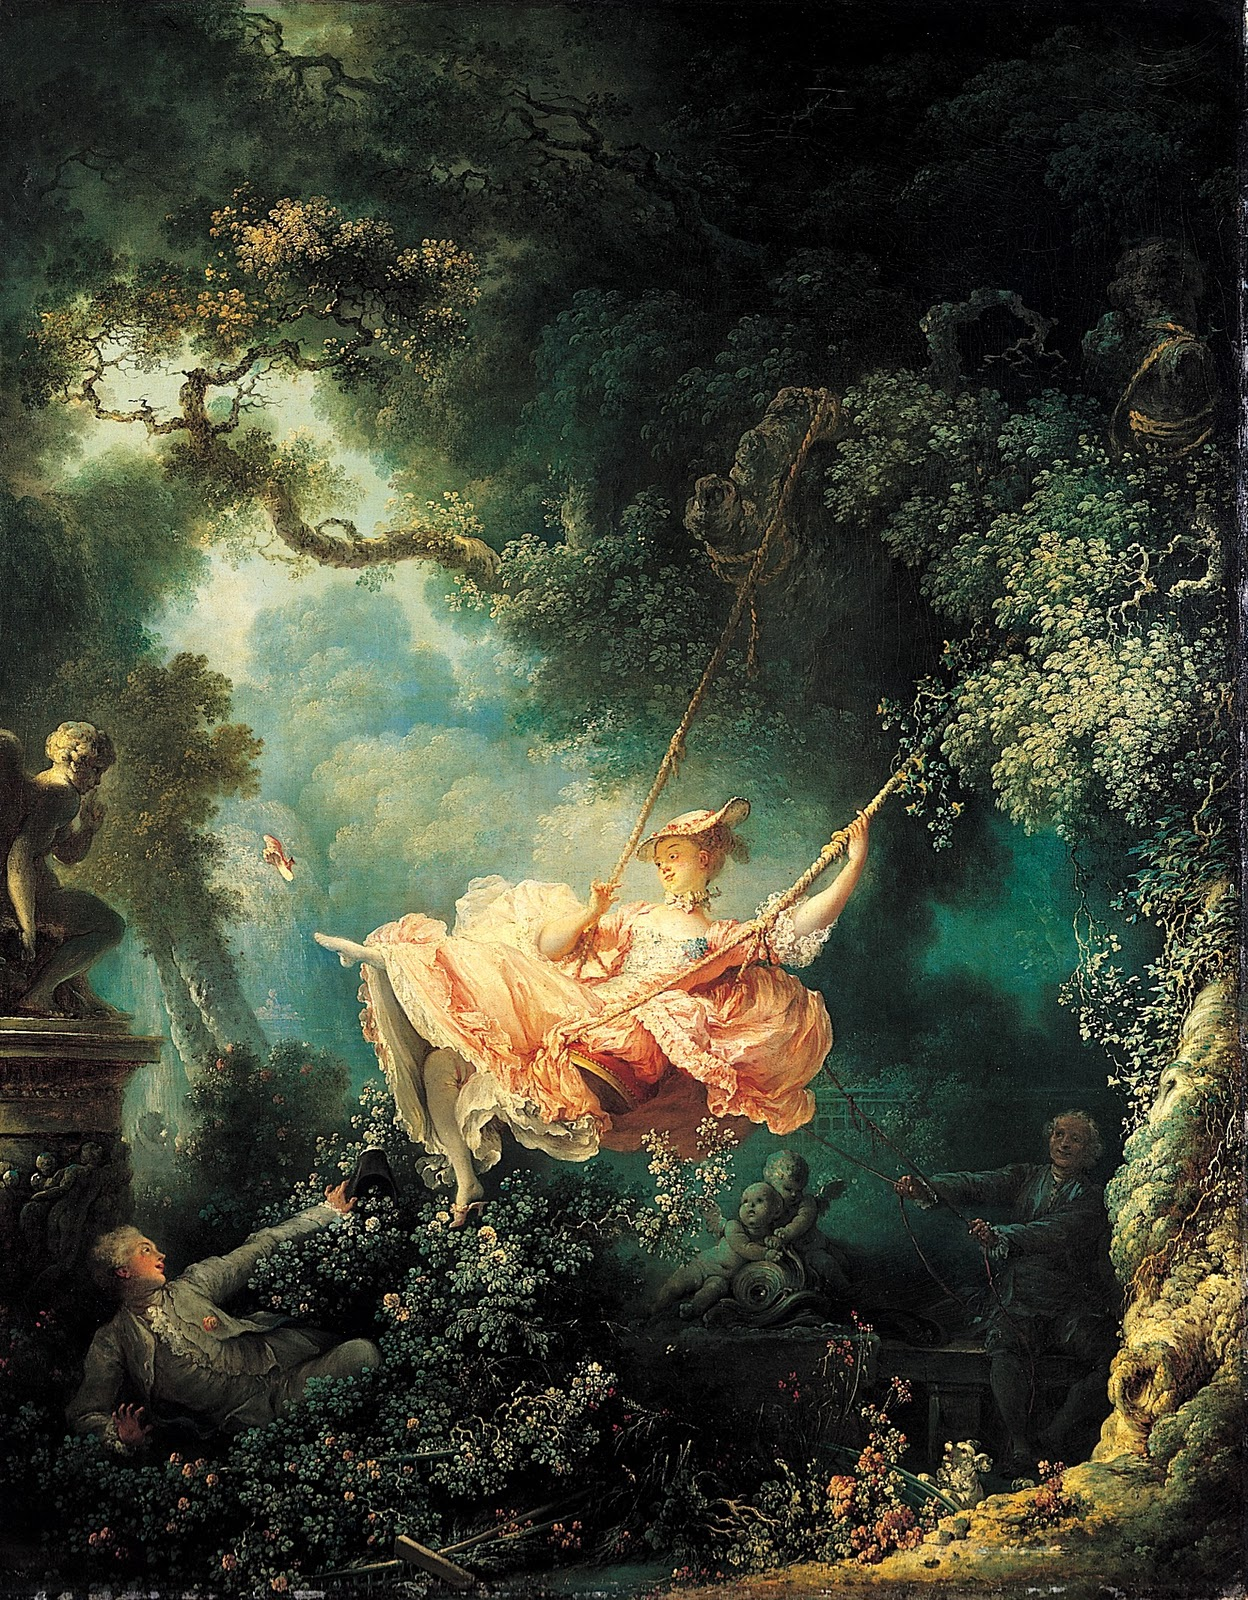
\includegraphics[scale=0.4, keepaspectratio=true]{qiuqian.jpg}
  \caption[让·奥诺雷·弗拉戈纳尔:《秋千》]{让·奥诺雷·弗拉戈纳尔:《秋千》。1767 年。布面油画。}\label{fig-qiuqian}

\end{figure}


\chapter{草稿之一——生命}

\begin{quotation}
  生命权是最基本,最重要的人权,如果无法充分保障人的生命权,那么一切其它权利都是
  空中楼阁。无端剥夺人的生命,或者肆意对人施加恐吓、虐待和折磨,就是用一种非人权
  的待人方式。任由这种情况发生,个人权利就无从谈起。所以一般各国的刑法都将侵害他
  人生命权的罪行量刑最重。

  生命权是一个人之所以被当作人类伙伴所必须享有的权利。\cite{renquanwiki}
\end{quotation}

\section{关于无国界医生的一场争议}

\begin{quotation}
  无国界医生是一个独立的国际医疗人道救援组织,致力为受武装冲突、疫病和天灾影响,
  以及遭排拒于医疗体系以外的人群提供紧急医疗援助。无国界医生只会基于人们的需要提
  供援助,不受种族、宗教、性别或政治因素左右。
\end{quotation}

笔者整理的不完整的中国内地无国界医生(MSF)成员名单(包括医生与后勤人员,按姓名拼
音排序,排名不分先后)阿依夏·那万、安娜、柴溪、蒋励、潘渊、屠铮、王娅王俊(夫妇二
人)、魏钊华、赵一凡、张定宇、曾思斌、周吉芳、邹纬等等。实际人数应为30人以上。笔
者向这些致力于在最恶劣环境下拯救生命的仁人志士致以我个人最大的敬意!
\improve[inline]{跟MSF联系下,看能不能要到名单}

MSF(无国界医生)首位中国内地成员是潘渊,他于1998年就加入了MSF,才开始时做中国境
内志愿工作,于2001年2月作为MSF首位来自中国内地的\textbf{海外}志愿者赶赴苏
丹。\cite{panyuan}

2006年,潘渊鼓动他的表姐——当时正在北京大学人民医院医学部任职妇科主治医师的屠铮加
入MSF。2007年3月,屠铮作为MSF医生赶赴利比亚执行为期半年的救援任务。成为中国内地首
位参与无国界海外救援项目的医生。\cite{tuzheng}
\unsure[inline]{据说至今为止,屠铮参加过5次海外项目了,需确认}

传媒、文学作品等往往将MSF成员描绘为在枪林弹雨里冒着极大生命危险抢救难民的英雄。
这是过于煽情而有失偏颇的,因为MSF医生的生命同样是生命,MSF组织并不会倾向于让医生面
临随时死亡的危险,而是在危险省份中的安全区域为难民实行救治。

在互联网舆情方面,关于MSF的讨论话题很少,单个话题的讨论人数基本都在10人以下,只有
知乎网的关于蒋励的一张帖子热度较高,文字回复条数过千。题目是,《如何看待北京医生
辞职去阿富汗参加无国界医生?》。\cite{kandaijiangli}

蒋励在北京大学医学部完成八年本硕博连读教育后,顺利入职北京大学人民医院。受师姐和
领导屠铮影响,“2012年参加了无国界医生。2013年3月至6月在无国界医生位于阿富汗霍斯
特的妇产医院工作(同时前往阿富汗的另一MSF中国内地成员——麻醉医生赵一凡去了昆都士省
的外科创伤医院),2014年1月再次去往无国界医生在巴基斯坦蒂默加拉的医院工
作。”,\cite{jiangli}。阿富汗霍斯特医院情况总结如下,床位\textbf{60}张,每
月\textbf{1200多例}分娩,相关医护人员有\textbf{2位妇产科医生,4位国际助产士,2位
  麻醉医生}组成,也就是说,这8个人彼此协作,24小时不间断的进行每天平均40余例的分
娩“流水线作业”。挽救了极多数量的新生儿和妊娠母亲的生命

但有关这个帖子的一些回复真是让人完全意想不到,瞠目结舌。其中点赞1700多次、点赞次
数排行第四的匿名帖子反对无国界医生对阿富汗的援助,提倡\textbf{绝育论},“已经生育
三个及其以上孩子的妇女向援助医院请求接生必须以切除子宫或者上节育环作为交换条件,
然后由国际组织建立隔离带,优先为已经绝育的妇女及其子女提供庇护,食物,医疗和基础
教育,把儿童从中剥离出来接受现代教育。”,有帖子发表类似观点“没有条件接受教育的
人就没有出生和生存的权利。”,除此之外,还有“愚善”,“学医救不了阿富汗”等脑沟
回清奇的言论。

在网络上,不止此贴所涉及国家,我们还可以看到,关于罗姆人(吉普赛人)、社会底层人
士的优生学绝育论。这种绝育论宣扬,就缺乏教育和社会资源的群体,或者相比自己群体拥
有更高不和谐的群体——这种水平判定其实只是个人不负责的主观判断,应当尽量抑制他们彼
此间繁殖新生生命,对于正在或已经出生的新生生命,“社会上流人士”有义务、有必要剥
夺新生儿父母的监护权、教育权,让社会特殊的学校或机构行使监护权、教育权,使他们脱
离这个不文明的群体……

\section{“科学”的优生学绝育论}

优生学常是举着科学的旗号,被一些别有用心或者精神脆弱之人利用,行反伦理、反人类之
实,让我们看看优生学在历史上曾被误用滥用的历史吧,以下内容节选自邱仁宗所著《一本
医学家、遗传学家、决策者和立法者必读的书——《从“安乐死”到最终解决
》》\cite{yousheng}:

\begin{quotation}
  
  1881年Francis Galton提出“优生学”,当时被定义为“通过优化生育改良人种
  的科学” 。于是在北美和欧洲兴起了一场将弱智、残疾、在竞争中处于劣势的人绝育、禁止他们第
  一章探讨种族灭绝的意识形态背景, 即固守“人类不平等”入境的优生运动。1907年美国印
  第安那州颁布了第一部将精神病人、性罪错者、智力低下者、道德堕落者和癫痫病人绝育的法律,到了30
  年代中期已有半数以上的州通过了类似的法律。

  对日耳曼人或德意志人的优良品质深信不疑的德国医生和科学家提出了“种族卫
  生”(Rassenshy giene)概念。

  1920年德国律师Carl Binding和医生Alfred Hoche出版了第一本题为《授权毁灭不值得生存
  的生命》的书。

  正是纳粹政权使种族卫生计划成为现实,它决心保持德意志血统的纯洁性,清理德意志的基因
  库,将“人类不平等”这一思想制度化。1933年7月颁布《 防止具有遗传性疾病后代法》,即
  绝育法,对患有各类精神和肉体疾病的病人实行强制绝育。1933年11月颁布《反危险惯犯法》
  和《安全和改革措施法》, 授权将反社会者关进国营医院,对性犯罪实行阉割手
  术。1935年9月颁布《 帝国公民法》和《德意志血统和尊严保护法》,二者统称纽伦堡种族
  法,正式在法律上排斥犹太人、吉卜赛人、黑人。

  1939年10月,希特勒签署了一份文件,文件称:“一些根据人道的判断被确认为不可治愈的病人
  在确诊后准许被实施慈悲死亡。”

  后来将残疾人安乐死的计划进一步在德国占领区扩大实施。接着大规模屠杀吉卜赛人和犹太
  人,进行所谓“最终解决”,被杀害的人数达600万人。
\end{quotation}

在数年前,这种极端蔑视生命权的言论在中国没有一丁点市场,几乎见不到有人去支持或宣
扬。如今我们不需要在网络上,就算是在现实中的社交场合,都可能会听到这些优生学绝育
论或灭绝论。你若反驳他们,这些少数派反倒会讽刺你为“\textbf{圣母}”。宗教、种族、
底层,我们为什么回到了,甚至超越了纳粹曾经的邪恶呢?我们忘了我们历史上被称为“东
亚病夫”“黄皮猪”的种族言论了吗?那在当时我们是不是应该被理所当然的消灭呢?

\section{被漠然视之的生命权}

一些老司机告诉我们“把人撞成重伤,不如直接撞死人”的言论,并有撞到陌生人后多次碾
压致受害者死亡的多个现实案例;笔者也在现实生活中听闻,施工工头第一时间将重伤建筑
工人送至医院,而得到了乙方负责人的怒斥,因为这增加了花销;某地的同胞们学习电影
《盲井》,整村组团外出靠矿井下杀人获利并组成犯罪链条;部分军事爱好者们狂想爆发战
争,中国重锤他国或地区,这是他们的民族自信啊;我们还可以看到一些所谓的左派们希望
重回激进,工运、革命,一些所谓的右派们想着引进西方的“民主”和“自由”,这些人在
他们自我标榜的方面常是狗屁不通,但都有个共同点就是不惜爆发战争,全国大乱,生灵涂
炭,在他们看来,大量生命面对困境或者死亡这种残酷性是“实现伟大梦想”所必不可少、
不可或缺、不能避免的。

宣扬这些反生命文化的不是未受教化、恶贯满盈之人,而更多是接受(过)高等教育的普通
人群,有些人甚至是博士。笔者认为,这反映出我国在关于生命权,关于正义和权利的社会
科学教育方面,是严重失位的,存在着可怕的匮乏与空洞。社会上下主抓经济建设的快速发
展,而将社会人文教育远远抛在了后面,有时这种反差甚至是故意为之。这些极端反生命权
的言论因此得以抬头,这真是对“中华上下五千年传统文明”的莫大讽刺。长此以往,即使
经济保持快速发展,即使我们自然科学知识获得了世界领先,我们仍将成为人类社会文明的
荒漠,荒漠中将只有个别人聊以自慰的小绿洲,而这小绿洲于国于家并无多大用处,只可自
慰而已。这最终仍会反过来导致经济、科学的大幅倒退。

\section{20世纪的战争}

我们迅速的将中国20世纪所经受的各种生命惨剧忘却脑后,而中国是20世纪因战争和暴行受
害最大、死亡人数最多的国家,其实离我们最近的一场战争——1979年中越战争,从爆发之日
算起距今算起还不到40年。马修·怀特(Matthew White)\cite{mattwhite}致力于研究和统
计战争及暴行导致的人类死亡人数,他采用科学做法参考多种资料,立场比较中立,数据统
计相对详实可信。虽然如此,因西方世界中战争及暴行相关参考资料大多带有反苏反共反中
的意识形态影响,这无疑也会使马修所使用参考文献的数据出现偏差,仍建议大家批判性地
接受。我们就用马修·怀特的数据来结束“生命”这一节吧。

% 表格设计URL:http://www.tablesgenerator.com
\begin{table}[h]
  \centering
  \caption{20世纪死于战争、屠杀和压迫的人数统计表}
  \label{20stdied}
  \medskip
  \begin{tabular}{@{}llllll@{}}
    \toprule
    & 战争军事死亡 & 战争平民死亡 & 大屠杀   & 饥荒    & 合计 \\ \midrule
    战争时期        & 3700万  & 2700万  & 4100万 & 1800万 & 12300万      \\
    和平时期        & 0      & 0      & 4000万 & 4000万 & 8000万       \\ 
    合计         & 3700万  & 2700万  & 8100万 & 5800万 & 20300万      \\ \bottomrule
  \end{tabular}
\end{table}

另外,依据马修其他页面,统计如下,第一次世界大战(1914-1918),全球死亡人数
约1500万。第二次世界大战(1939-1945),全球死亡人数约6600万。20世纪全球全部死亡人
数大约为55亿,其中死于20世纪战争、人类暴行的人数约2.03亿,也就是说,在20世纪,全
球死亡人口中平均每27人中就有1人死因是战争或人类暴行。

中国方面,军阀战争(1917-1928)期间各方军队战死约20万,因屠杀和饥荒死去的民众
约60万,共计死亡约80万。第一次国共内战(1928-1937)期间,死于战争、屠杀和饥荒的军
民约500万。抗日战争(1937-1945)期间,国共两党军事死亡人数约180万,平民死亡人数
约800万,伪军死亡人数约20万左右,合计死亡约1000万人。第二次国共内战(1945-1949)
期间军民死亡人数约250万。

\section{“人相食”的中国史}

在中国史书记载上,“人相食”屡次出现,已经成为一种固有表述\cite{renxiangshi}。据
不完全统计,《资治通鉴》中大约平均30多年出现一次人相食,《二十四史》中因记录
详细,跨越朝代久远,大约20多年出现一次人相食。

在《中国古代的食人》一书中,郑麒来(美籍韩裔)将食人分为两类,“求生性食人意味着
人们为自己的生物性生存而互食,与求生性食人密切联系的食物匮乏往往由战争、内乱等人
祸或干旱、饥馑、虫灾等天灾引起。习得性食人……更多受制于文化因素,诸如爱与
恨。”\pagescite[][152]{9787500415480}。“在研究中国历史文献的过程中,我们发现
153例与战争(直接)有关的食人事例,均由战时或战后的饥饿和饥荒引起。……间接相关的有
74例,两个数字加起来,即全部与战争有关的食人事例便共有227例”。(个别案例有重复,
还有个别案例因不具统计意义也没有计入统计。),几乎每朝每代均发生这种求生性的群体
人相食。这些统计数据并不包括地方方志所记载的“人相食”。

综观人类历史,就民计民生方面来说,人类很可能不是总体向上进步的螺旋上升,而是因欲
望带来的生发死灭,与之相伴的悲喜交加的上下循环。且在这欲的循环中,向上的、喜剧的
经历苦短而观众甚少,常常是你方唱罢他登场;向下的、悲剧的经历恨长而观众众多,常常
是意悬悬半世心,枉费了卿卿性命。难道说福柯是对的吗?
\begin{quotation}
  人性并不会在持续不断的斗争中逐渐进步,直到最后达到普遍的互惠,最终以法律准则取
  代战争;相反,人类将其每一种暴戾都深深地潜藏于法律体系之中,因而所谓人性的进步
  只不过是从一种统治形式过渡到了另一种统治形式而已。
\end{quotation}


笔者认为,对于人类,尤其对于中国人来说,我们对于生命的认知和尊重在总体上很可能仍
是处于较低水平。我们很可能会将“岁大饥”、“人相食”在未来的某一天继续下去,再次
书写食人的历史,因为我们的历史几乎没有一个朝代不曾发生“人相食”。至于那在哪一天,
是否一百年、二百年后,那就不知了。当前来说,幸好前人与我们现在的人何干,而我们本
身也善于遗忘。幸哉乐哉!\bigskip


朋友们,我们下次战争再见吧。


\chapter{草稿之一——工作制}

(Warning:医疗行业加班比较特殊,涉及国家社会保障方面,不是单纯的超长加班问题。我
对医疗行业完全不了解,没有办法写。有医疗相关从事人员或了解医疗行业的人可以与我联系。)

\section{传统超时加班企业}
在中国,劳动密集型企业是我们传统的超时加班重灾区,在制造业这种现象更为严
重\cite{guojilaogongshijian},曾经引发社会极大关注的富士康连续跳楼事件便被认为是
因超时加班所致,仅2010年一年被媒体曝光出来的就有“14连跳”。富士康为降低、杜绝此
类事件采取了一系列举措,2010年、2011年两次大幅提升工资、建全加班制,铺设大面积防
跳楼网,签订《不自杀协议》……2011年后,就很少有相关报道了。

根据《富士康工资、工时与生产管理调研》\cite{fushikangzuixin}一文,虽然至2015年为
止,富士康工人超时加班现象仍较严重,但大量裁员现象却与之并存。“2013年媒体又报道
了富士康新一轮的变相裁员浪潮(在2013年富士康全国用工规模减少了21万),引起工人
以`跳楼'”或停工等形式的激烈反抗。”。2016年,BBC发文报道《富士康用机器人取代
了6万名工人》。至于为何会发生超时加班与严重裁员并存的情况,我们放在下
面“\nameref{sec:gzryuanli}”一节中再做整理。

\section{新型超时加班企业}
金融和互联网企业是二十一世纪新加班重灾区。华为的“加班文化”流传甚广,有很多段子。
华为苏州研究院椅子背后常备的睡袋,酷爱加班文化的日本专家入职华为两个月后愤而辞
职“你们这样是不人道的”,华为总裁任正非挽留要回北京陪妻子的副总李玉琢时说“这样
的老婆你要她干什么?”,还有任正非对另起炉灶的李一男的“追杀令”最终迫使李一男重
回华为。华为在舶来词方面有个贡献,将日本“过劳死”的概念成功传播到了中国。

说起创意,华为也一点也不比富士康《不自杀协议》差。我国于2007年6月29日颁布《劳动合
同法》,其中第十四条规定“有下列情形之一,劳动者提出或者同意续订、订立劳动合同的,
除劳动者提出订立固定期限劳动合同外,应当订立无固定期限劳动合同:(一)劳动者在该
用人单位连续工作满十年的……”。这个法案将于2008年1月1日正式实施,在2007年底,华
为安排7000余名工龄8年以上的老工人向公司递交自请辞信,作为补偿,华为向这些老工人支
付约十亿元违约金,然后再重新聘用这些“失业工人”,工龄从零开始重新计算。数天
后,2008年1月1日,工人们“自愿”为了几万到十几万的补偿金,放弃了订立“无固定期限
合同”的可能,变为了1至3年劳动合同的新工人。“华为裁员门事件后,沃尔玛、环球、摩
托罗拉等公司也先后进行了应对新法的人力资源调整。《劳动合同法》实施前的“阵痛”似
不减反增。\cite{huaweimaiduan}

2010年8月,华为“公司14级以上工人被要求`自愿'签署《成为奋斗者申请书》……申请“华
为奋斗者”有一个必备条件,需要添加“我申请成为与公司共同奋斗的目标责任制工人,自
愿放弃带薪年休假、非指令性加班费和\textbf{陪产假}”这句话。\cite{huaweifendou}华
为真是个互联网企业的好模板。

任正非在2001年有篇文章《华为的冬天》非常有名,当时国内大公司似乎基本没有这
种“Winter is coming”的论调,更无一认为自己可能马上狗带。任正非的危机意识立刻被
广大媒体、企业称赞。近20年过去,在这种强烈的危机意识下,华为仍是高奏凯歌、一路前
行。而2017年,一些年过34岁的交付工程维护人员,过40岁的研发员工和45岁的老员工却可
能迎来了真正的凛冬,要被清退掉去他处过日子了。当然,华为已经惯例辟谣了。据说当前白色
家电企业也已经开始学习华为,对34岁工程师劝退……

2016年8月29日起,58公司总裁兼CEO姚劲波的微博陆续被众多58公司工人、工人家属和社会
人士浏览并情绪不稳定地评论\cite{tai58},起因是58公司在不发邮件和公文的情况下口头
传播了公司新工作制度——“996工作制”,早九点上班,晚九点下班,星期六正常上班,没有
任何补贴。虽然这种工作制可能并非58公司原创,但却是由因它开始引起公众反加班的社会
影响,并且在事件后,“996工作制”并没有受到实际影响,反而成为了一种明目张胆的制度。
笔者认为,58公司“996工作制”这一事件,可以定为中国劳动制度的一个里程碑。这标志着
严重超时工作制从原来只是个别公司内部隐性文化、不成文规定,发展至显性公司制度,并
最终成为一种公开的可以被任何企业复制的社会劳动制度。

滴滴出行于2016年底连发三篇大数据报告《2016年度加班最“狠”公司排行
榜》\cite{zuihen},涉及金融、互联网、公关、广告四个行业,包括33家公司。这33家公司
中最晚下班时间均在20点后,其中20点到21点之间下班的只有15家。四个行业相比较,工作
日时长方面金融行业较好,互联网业最差,最高加班时间是京东23点16分。周末上班方面,
金融业最差。0-5点下班返工人数方面,公关、广告公司表现突出,其中奥美广告返工人
数3080人,金宝大厦3家公司合计2102人。

\section{工作时长立法}

去看二十世纪或者当前的劳动法已经是难堪之事,那让我们粗略看下最早期的工时立法吧。

英国全行业立法是始于“1874年,R. A. Cross提出工厂方案,最终使得所有的英国工人都享
受10小时工作的权利”\pagescite[][96]{britishworkday}。

法国一步到位,直接是全行业立法,“法国1850年9月5日的十二小时工作日法令是临时政
府1848年3月2日法令的资产阶级化的翻版;这个法令适用于一切作
坊”\pagescite[][319]{capital}。

我们这些大体量的企业,靠着不懈的努力,向前150多年终于赶超到了英法19世纪中后期水平,
真是可歌可泣。另外,24小时工作制其实也已经来了,就是工作、睡觉、起床接着干活,一
天24小时不离公司,祝这些企业能早日赶超到19世纪早期劳动水平吧,就是不知道是否还需
要童工呢?

结合实际来看,我国现在实行的1995年劳动法,规定的8小时工作制相比其他各国标准较高,
要求劳动时长较短,比德国、新加坡等一周60小时工作制还要少不少。在实际操作上缺乏一
些空间,可能的解决方案如弹性工作制、休息权等问题还在探讨中。希望尽快出台相关政
策。

\section{超时加班的危害和原理}
\label{sec:gzryuanli}

对于超长劳动时间的论述和批判,首推马克思。希望大家能摆脱对马克思或褒或贬的刻板印
象,单从理论本身出发判断而不是意识形态的肯定或否定。

150多年前的《资本论》中提到的一些情况,居然仍高度适用我们的当前社会,在世界发展
方面来说这真不是一件庆幸之事。那么为何我们又重新回到150年前的工作状况?笔者认同大卫·哈维的说法——因新自由主义的盛行。

马克思原文如下(不想看马克思原文的读者,可以略过这部分):
\begin{quotation}

  至于个人受教育的时间,发展智力的时间,履行社会职能的时间,进行社交活动的
  时间,自由运用体力和智力的时间,以至于星期日的休息时间,——这全都是废话!但是,
  资本由于无限度地盲目追逐剩余劳动,像狼一般地贪求剩余劳动,不仅突破了工作日的道
  德极限,而且突破了工作日的纯粹身体的极限。\pagescite[][306]{capital}

  《1861年爱尔兰面包业委员会的报告》中提到,“委员会认为,把工作日延长
  到12小时以上,是横暴地侵犯工人的家庭生活和私人生活,这就侵犯一个男人的家庭,使
  他不能履行他作为一个儿子、兄弟、丈夫和父亲所应尽的家庭义务,以致造成道德上的非
  常不幸的后果。12小时以上的劳动会损害工人的健康,使他们早衰早死,因而造成工人家
  庭的不幸,恰好在最必要的时候,失去家长的照料和扶持。”\pagescite[][292]{capital}

  工人阶级中就业部分的过度劳动,扩大了它的后备军\footnote{想在本行业入职的失业或
    半失业人}的队伍,而后者通过竞争加在就业工人身上的增大的压力,又反过来迫使就业工
  人不得不从事过度劳动和听从资本的摆布。工人阶级的一部分从事过度劳动迫使它的另一部
  分无事可做(无事可做指后备军),反过来,它的一部分无事可做迫使他的另一部分从事过
  度劳动,这成了各个资本家致富的手段,同时又按照与社会积累的增进相适应的规模加速了
  产业后备军的生产。\pagescite[][733]{capital} 

  决定工资的一般变动的,不是工人人口绝对数量的变动,而是工人阶级分为现役军和后备
  军的比例的变动,是过剩人口相对量的增减,是过剩人口时而被吸收、时而又被游离的程
  度。\pagescite[][733]{capital}

  产业后备军在停滞和中等繁荣时期加压力于现役劳动军,在生产过剩和亢进时期又抑制现役
  劳动军的要求。所以,相对过剩人口是劳动供求规律借以运动的背景。它把这个规律的作用
  范围限制在绝对符合资本的剥削欲和统治欲的界限之内。”\pagescite[][736]{capital}

  不变资本的固定部分即工厂建筑物、机器等等的规糕,不管用来工作16小时,还是12小时,都
  会仍旧不变。工作日的延长并不要求在不变资本的这个最花钱的部分上有新的支出。此外,固
  定资本的价值,由此会在一个较短的周转期间系列中再生产出来,因而,这种资本为获得一定
  利润所必须预付的时间缩短了。因此,甚至在额外时间支付报酬,而且在一定限度内甚至比
  正常劳动时间支付较高报酬的情况下,工作日的延长都会提高利润。因此,现代工业制度下
  不断增长的增加固定资本的必要性,也就成了唯利是图的资本家延长工作日的一个主要动
  力。\pagescite[][91]{capital3} 

  资本主义生产方式按照它的矛盾的、对立的性质,还把浪费工人的生命和健康,压低工人的
  生存条件本身,看做不变资本使用上的节约,从而看做提高利润率的手
  段。\pagescite[][101]{capital3}
\end{quotation}

以上意思是指:
\begin{enumerate}
\item 工人、职员异化成为企业身上一个微小的、易损坏和易更换替代的一个器官。不止个
  人的健康、生命受到损害,他的社交角色、儿女角色、父母角色、夫妻角色等社会角色则
  被严重削弱和抑制。由此会引发什么问题呢?在中国传统的家庭人伦关系上,难以孝敬、
  赡养老人,难以增进夫妻关系,难以同子女产生良好沟通和教育,家庭组建、生儿育女的
  时间也都会滞后许多。尤其是华为《奋斗者申请书》居然明目张胆“自愿”要求放弃本就
  不多的陪产假,真是反基本社会人伦,千夫可指。当然,华为始终横眉冷对,淡定得很,
  人家负面新闻也像富士康一样越来越少了,这真是进步呵!

\item 在职工人、职员的过度劳动,使当前就业人数相对于正常劳动情况下应当就业的人数
  减少了。当前未就业或者半就业工人、职员的存在又使在职工人、员工的工资报酬被压
  低。

\item 随着生产力发展,机器等固定资本的支出愈加巨大,不管其使用或不适用,都在产生
  折耗,这是生产力发展所必要的。为了事实上节约这种固定资本,就需要延长工人劳动时
  间,这就使工人超长劳动似乎成为一种生产力发展的必须。另外,如果雇佣更多工人,则
  需要更多数量和更大投资的固定资本,这对本已庞大的不变资本支出无异于雪上加霜。

\item 此外,脱离马克思文本,就实际情况来看,通过超长工作日所产生的工人、职员数量
  节约,使企业培训成本、培养成本、管理成本、福利保障成本、风险成本均大幅降低。

\end{enumerate}

综上,企业倾向于让员工尽量加班而非在原工作时长不变的情况下雇佣更多工人。

那么工人、职员为什么要加班呢?(Warning:这里感觉还很单薄,希望读者能与我联系,
提供宝贵建议和意见。)
\begin{enumerate}

\item 如富士康这类工厂,将基本工资设的较低,工人的工资财富积累常常只能在加班费中
  来完成。不加班,不赚钱。加班了,才有钱。这是两百来年很多大工厂惯用不变的伎俩。
  或者如华为将部分加班费融合进了工资,一些职员由此认为工资是可观的。这两种情况其
  实都是一样的,就是企业确实补贴了部分工资。但工人、职员本应得的远比实际得到的其
  实要多的多。

\item 如华为这类企业,已在社会具有相当的名声。大众普遍认为能进华为的,肯定是有一
  定水平的。能在华为干住的,跑到其他企业肯定是不怕累的。在一些职员看来,被压榨就
  压榨吧,加班就加班吧,一个跳板而已。撑过现在,未来是光明的。

\item 企业考核。不管是领导思想上的还是落在纸上的考核,都将加班量作为职员是否合格
  的一个标准,华为有个词很有意思,叫“工作量饱满”。工作量不饱满,你就不是个称职
  的员工。工作量饱满了,员工的个人时间,家庭时间也就别想饱满了。

\end{enumerate}

员工作为这个微小的、易损坏的、易更换替代的工厂、企业小器官,在被榨干后,甚至只是
在自己年龄增大后、工龄福利增多后,就将迎来自己被扫地出门的结局,他们将被年龄更小,
福利待遇更低的年轻员工所取代!超长工时所带来的利润诱惑是极易在工厂、企业间传染的。
这便是自由!实则是资本的自由,而非人的自由!

\section{工时改革问题的民族国家与全球化困局}

重新结合实际情况立法,对工人、工会赋权,加入弹性工作制和阶梯性休假等补偿措施,加
大执法力度,主动执法,对较重违规现象进行惩罚性罚款等,这些举措理论上将能有效解决
工时严重过长的问题。

就以往传统历史经验来说,19世纪英国工作日改革经验表明,“劳动生产率和劳动强度的变
化,或者是在工作日缩短以前,或者是紧接着在工作日缩短以后发生
的”\pagescite[][601]{capital},后来福特8小时工作制以及世界上广泛传播的劳动法均在
一定程度上证明了这点。

但现实是严酷的,我们可能无法去实行这些举措。因为立法要考量社会整体在立法后的整体
得失均衡。如果只是工人工时得到大的改善,导致其他方面造成矛盾激化,对国家、企业甚
至工人自己产生比立法之前更为恶劣影响的话,就不符合科学立法的精神。笔者认为,传统
工时改革的成功依赖于国家政治地理上的整体性、一致性和封闭性,一旦颁布条令就覆盖全
国工厂、企业,工厂难以迁至他国,必须接受当前法律条令制约。而当前有一条横贯在工时
改革前的巨大矛盾就是,全球化对世界上各个民族国家均造成巨大压力,而中国工时改革必
将更为扩大这种压力。

安东尼·吉登斯在《现代性的后果》一书中提出,现代性的全球扩展趋向产生了一个“失控的
世界“,它的出现没有人也没有政府能够全面地控制。马克思用怪物来描述现代性,而吉登
斯将其比作坐在巨型汽车或”猛兽“上面。笔者认同吉登斯上面所言。所谓全球化,说穿了
就是资本在全球高速通畅的流动。不管是中国政府,还是美国政府,不管是工人还是大企业
家在面对全球化这一庞然大物时都常是有心乏力的。

全球化给中国工时改革,甚至是劳动改革所带来的巨大压力,主要表现为两个方面,
一个是东南亚、南亚、拉美劳动市场的低廉——相当程度上是因为贫困人口、童工、更贫穷国
家的劳动力输入,和法律不健全等引起;另一个是美国降低税收,大力吸纳国际企业和本国
企业进驻,制造业进驻的政策扶持力度也一直在扩大。以富士康\cite{foxconnwiki}为例,
其在巴西、匈牙利、斯洛伐克、土耳其、捷克、日本、马来西亚、墨西哥、印度、美国均有
工厂。印度方面已与富士康签订谅解备忘录,富士康预计在5年之内投资印度50亿美元,“美
国方面唐纳德·特朗普总统于2017年7月26日宣布,富士康将在威斯康星州东南部建立一个价
值100亿美元的平板电视制造工厂。威斯康星州将每年向富士康支付高达2.5亿美元的补贴,
为期十五年。这笔交易被一些人批评为是拿取30亿美元纳税人税收资助激励富士康。威斯康
星州立法机关的无党派预算办公室的分析确定,国家纳税人将在2043年收回投资。”

如果中国工时改革成功,工人劳动时间趋于正常,相关产业领头羊们很可能不会将重心放在
另想它法,提高劳动生产率上,以解决因工时恢复正常所带来的效益下降——而是转战早就已
经或者正在海外建设起来的基地。因企业实力不足、性质和特点限制而走不出去或难以走出
去的企业们则可能承担来自全球化国际市场的巨大竞争压力。届时中国除大规模资本逃离外,
将出现过多被产业抛离出来的,难以就业的真正剩余劳动力,造成社会问题。

此外,福耀玻璃董事长曹德旺宣称美国实际税收远比国内实际税收低廉。美国政府也配合其
支持取缔工会。这是美国政府给其提供的“胡萝卜”,但是他却没说“大棒”——美国政府为
吸引他国生产制造业等资本密集型工业进驻美国国内,所提出的关税、反垄断、反倾销威胁。
(Warning: 这方面希望读者提供更多有力确实资料)。这也是全球化面前,民族国家之间
的矛盾。

全球化给工时改革带来如此巨大压力,那么如何破局?如何尽可能的完善?笔者能力弱小,
所能做的可能只是提出以上问题了。国家目前已经越来越关注“构建和谐劳动关系”,让我
们拭目以待吧。

最后,用诗人许立志的一首诗来结束本节吧。

\poemtitle*{流水线上的兵马俑}
\settowidth{\versewidth}{Than Tycho Brahe, or Erra Pater:}
\begin{verse}[\versewidth]
  沿线站着\\
  \qquad 夏丘\ \qquad \quad  张子凤\qquad  肖朋\\
  \qquad 李孝定 \qquad  唐秀猛\qquad  雷兰娇\\
  \qquad 许立志 \qquad  朱正武\qquad \\
  \qquad 潘霞\  \qquad \quad 苒雪梅\\
  这些不分昼夜的打工者 \qquad 穿戴好\\
  \qquad  静电衣 \qquad  静电帽  \quad  静电鞋\\
  \qquad  静电手套 \quad 静电环 \\
  整装待发 \quad 静候军令\\
  只一响铃功夫\\
  悉数回到秦朝
\end{verse}
\newcommand{\attrib}[1]{%
  \nopagebreak{\raggedleft\small #1\par}}
\attrib{许立志 (1990--2014)}


%%% Local Variables:
%%% mode: latex
%%% TeX-master: "../main"
%%% End:


\part{国家}

\chapter{草稿之一——维基解密、阿桑奇与西方政治}

\section{维基解密简述}
维基解密官网的域名wikileaks.org注册于2006年10月4日,朱利安·保罗·阿桑奇一般被视为
其创始人。自维基解密成立之初,就着力于解密大批文档。创始之初采用公共编辑方式,任
何人都可以发布、修改页面。后来改为只接受具有政治、外交、历史或伦理意义的文件,所
提交文件需要匿名维基解密工作人员的审阅。

维基解密在十年多的时间里,多次对世界造成巨大影响。如公布肯尼亚原总统腐败案;阿尔
及利亚政府与石油公司合作,破坏另一家石油公司的设备造成石油大面积泄露;伊拉克战争
美军直升机射杀平民,包括两名路透社记者和儿童;阿富汗战争的大量文件及关塔那摩虐俘;
美国、俄罗斯的可以侵入几乎涵盖所有系统的网络黑客工具等。

\section{希拉里邮件门事件}
在2016年,维基解密先后发布10多万封有关于希拉里的邮件,一般被称为“邮件门”,影响
更是巨大。本节内容有借鉴以下网页。
\begin{enumerate}
\item \href{https://www.zhihu.com/question/41676600}{知乎:DNC邮件中有哪些美国民主党不可告人的内容?}

\item \href{https://www.zhihu.com/question/51362588}{知乎:如何看待The Podesta Emails?}

\item \href{https://github.com/zhouningyi/us_selection_crack}{GitHub:希拉里邮件
    门数据}
\end{enumerate}


为力求客观表述,克林顿基金会连续杀人、撒旦教披萨门等经由网友讨论演绎出的
阴谋论不计算在内,只节选其中极少数邮件和与之相关的后续发展如下。

2016年3月16日,维基解密发布30322封希拉里邮件,邮件收发时间跨度为2010年6月至2014年8月。

2016年7月22日,维基解密发布19252封DNC邮件,邮件收发时间跨度为2015年至2016年5月25日。
\begin{enumerate}
  \item emailid/25 希拉里竞选团队用邮件向DNC(民主党全国委员会)确认已收到几张DNC支
    票,被Jordan Kaplan严厉斥责:“不要再像这样发邮件。你认识Alex(直接跟他说)。
    不要犯蠢。”(根据网友分析,希拉里竞选团队通过HVF和DNC获取超过政治献金限额的
    捐赠,然后将超额捐赠化整为零,将这笔钱投入到广告或者通过小额筹款)
    
    \item emailid/1041 DNC中的Luis Miranda提供了造谣污损特朗普的几个方向。如特朗
      普危险、暴力、侮辱女性、穆斯林、墨西哥人、反对言论自由等。

      \item emailid/17065 富人Liz为HVF(希拉里胜利基金会)开具了一张20万美元的支票,要求希拉里参加在
        美国驻联合国人权理事会大使Eileen Donahoe家中举办的私人晚宴。
        
  \item emailid/20352 Jordan Kaplan要捐赠人名单,要求将名单发给Scott Comer。这些
    人有可能进入USPS, NEA, NEH等董事会,但也有可能进入不怎么好的董事会、理事会,
    如美国妇女历史委员会。

  \item emailid/658 Scott Comer提供了一个23名捐赠人名单。(据知乎帖 \url{https://www.zhihu.com/question/41676600},有部分人的捐赠数额,除去捐款最少的25美元和2600美元外,数额均在4万美元以上,最多捐款额为334000美元。)
\end{enumerate}

2016年10月7日,维基解密发布58000余封John Podesta的邮件。
Podesta于1998-2001年任比尔·克林顿的白宫幕僚长,2014-2015年任奥巴马总统顾
问,2015-2016年任希拉里竞选团队主席。
\begin{enumerate}
\item emailid/8396 2011年,卡塔尔邀请克林顿参加了纽约一个5分钟的小会,并承诺捐赠
给克林顿基金会100万美元,作为克林顿生日礼物。另外,卡塔尔对希拉里提出的海地投资
意见表示感谢,会加以考虑。

  \item emailid/7452 比尔·克林顿的幕僚长Tina Flournoy致信Podesta,外国政府捐赠
的钱已经入账。

  \item emailid/22030 摩洛哥提出向克林顿基金会支付1200万美元,但有条件——希拉里要
于2015年5月出席在摩洛哥古城马拉喀什为其召开的“克林顿全球倡议大会”,并在大会发
表演讲。(这在希拉里工作过的美国国务院已构成受贿行为,但希拉里仍然收下了这笔钱。
因担心影响选情后由其丈夫比尔·克林顿和女儿出席)

  \item emailid/6775 沙特谢赫穆罕默德酋长(可能翻译有误)想对克林顿提供飞机使其
参加埃塞俄比亚的会议一事表示感谢,要求克林顿亲自致电给他。Podesta同意Doug Band的
意见:除非穆罕默德酋长向克林顿基金会捐赠600万美元。

  \item emailid/4635 Podesta在疑与普京高度相关的Joule Unilimited公司持有75000股
股票。(后于奥巴马任期2014年时将股票转让给一家匿名控股私人公司)

  \item emailid/57027 民主党国家委员会的临时主席,也曾任职于CNN的Donna Brazile,
向希拉里泄露其与桑德斯党内辩论时要被问到的两个问题.在其他邮件中,Brazile想在希拉
里总统胜选后做Podesta的代理人。

\item emailid/39107 Alphabet公司(Google母公司)董事长Eric Emerson Schmidt的一个
  小团队为希拉里竞选团队制作竞选页面工具,并搜集整理捐赠者信息、信用卡号数据库等,
  团队工作人员认为Eric Emerson Schmidt暗示他可以做的更“全面”。(
  据
  \href{https://www.opensecrets.org/lobby/clientsum.php?id=D000067823&year=2017}{Center
    for Responsive Politics}统计,Alphabet/Google政治献金数额极大,2017年总游说费
  用为1815万美元,游说人数102人。)

\item emailid/8190 2008年10月6日,时任花旗银行高管Michael Froman发给Podesta一封主
  题为“Lists”的邮件,要求名单上的人应当优先考虑出任政府高官。附件分为3个,第一
  个是92个女性名单,第二个是222个非白种美国人及残疾美国人名单,第三个附件为31个内
  阁职位或内阁同级职位提名名单(附优先级与候选人)。(2008年大选投票日期是11月4日,
  奥巴马当选后,有近半数入选奥巴马内阁。)

  \item 其他,近百位媒体工作者、领导被Podesta招待。多位记者向Podesta表忠心,还有
    人预先告知将会提问希拉里的问题或者在发文章前请希拉里竞选团队过目。
\end{enumerate}


\section{维基解密的理念}

综观维基解密历史,它的理念应当是显而易见的。通过世人关注,吸收多渠道泄密出来的超
大批量文件,不管信息来自哪个渠道——黑客、政府和企业工作人员、某一派系的敌对方都可
以,只要解密文件是真实的便可接受。当信息量大到一定量级时,这个系统就是高度容错的
了,泄密者、甚至网站管理人员的个人主观就不起作用了。原本泄密相关的具体、特殊个人
和事件就会一个个结合起来,构成为更富普遍性、一般性、客观性的权力和金钱光谱。世人
由此看到这种光谱可怕的反伦理反人类,从而谴责、批评、改造、审判这种反伦理,号召权
力相关信息的更加公开化,以让世界变得更加阳光美好、公正平等、符合伦理。

以邮件门为例,\$illary Clinton和她"still dicking bimbos at home"的丈夫比尔·林顿本
来只是带有个人特色和性格的两个人,作为人来说他们是特殊的、个别的,在竞选中则代表
一方竞选势力。但随着邮件量级的增长,我们可以将其抽象到民主党,再到美国政治、资本
生态,再到西方,直至抽象到人类整个的——可以是当前的,也可以是历史的——权力、资本生态,
甚至抽象到人欲本身。

\section{维基解密的缺陷及潜在问题}

本小节内容框架主要来自于知乎用户\textbf{@阿迦陀},感谢\textbf{@阿伽陀}的批评指导。

有人指责维基解密与俄罗斯政府有关联,如DNC邮件泄露被怀疑有俄罗斯政府官员参与其中,
向维基解密递交了邮件。也有人指责维基解密与特朗普有关联。如阿桑奇就曾在某次电视节
目上自带“Vote Trump”的胸标,在个别采访也倾向于川普。但在一次采访中当主持人问他
选择投票给特朗普还是希拉里时,阿桑奇又说“霍乱还是淋病的选择吗?就我个人而言,我
一个都不喜欢。”。还有美国总统特朗普的长子小特朗普在推特上发布过这样一条信息:小
特朗普从2016年9月美国大选期间到今年7月之间与维基解密在Twitter上的私聊记录。其中一
条信息显示,维基解密希望小特朗普帮忙——让特朗普总统建议澳大利亚指派阿桑奇为澳驻美
大使。笔者个人认为阿桑奇向特朗普的倾斜出自现实的考虑,以使自己不必腹背受敌,谋求
大使职位则是希望借助大使的外交豁免权来保护阿桑奇不受伤害。

\begin{enumerate}
\item 不受制约的权力困境:

  维基解密试图借助公开秘密文件,打击不受制约和暗箱化操作的权力,使政治、军事、外
  交、伦理奔向更为阳光的一面。在维基解密的历史中,它也已具备极高可信度。但同时,
  维基解密的内容发布权限只集中在少数几个人的委员会,甚至阿桑奇自己手中。在试图制
  约其他权力的同时,维基解密的“发布委员会”自身也具备了极高的权力,这种权力由维
  基解密各种直接或间接的用户所赋予。

  那么,由谁来制约维基解密自身的权力呢?在现实中,因其倾向于特朗普,也在一定程度
  上影响了大选结果。勇者要谨防成为恶龙,而我们却不能提供预防恶变的措施,只能单薄
  无力地寄希望于阿桑奇自己的个人人格。

  比较容易想到的方案就是公众监督执行,但这样又会回到早期维基解密“公共编辑”方式,
  陷入信息大爆炸,从而难以筛选、管制、保持重心和尖锐,有价值的和无价值的、真实的
  和虚假的都混杂在一起。这种困境最终会使维基解密失去其“真实有力”的核心价值。

\item 核心机密文件的筹码困境:

  维基解密在因特网上分几次释放了数十GB加密文件,解密密码掌握在阿桑奇手中,数年来
  从未公开。这些大量加密文件被认为是足以造成国家动荡的核心机密,而用来解密这些文
  件的密码也是阿桑奇的“保命筹码”。凭此筹码,美国等国家不敢轻易直接对阿桑奇采取
  极端措施。维基解密掌握的这些最为有力的文件,在非极端情况下却几乎永不会为人所知。

\item 体制外权力的限度困境:

  维基解密是一种反体制规训的强大力量,这种力量无法融入体制。它寄希望于通过公众的
  知情权,以“自下而上”的方式来打破规训,走向美好,至于怎样“走向”,是它所不能
  提出的。也就是说,它具有极强批判性,但是建设性还是有限。

  @阿伽陀认为体制仍是重要且现实需要的,维基解密太过于反对体制,只能被反对派、寄生
  虫和别有用心者利用,我个人对此持有限赞同态度。我的观点阐述在本文最后两段。
\end{enumerate}


\section{希拉里邮件门之后}
(Warning: 本节还没写完,刚开始。)

希拉里邮件门,特别是Podesta邮件曝光后,美国媒体先是相当沉默,直至在公众网络上此事
越炒越热后才真正介入,CNN居然有主持人说公众直接去看泄密邮件是违法的,公众应当从媒
体、从CNN获取“权威”的泄密邮件相关报道。Quora,4Chan,Google均有删除维基解密相关
内容的行为。本是希拉里对立面的特朗普也往往避重就轻,顾左右而言他,皮尽管扯,里子
却是触动不得的。媒体、政治地被规训在此表现的淋漓尽致。

那维基解密理念中所在意的世界大众的力量呢?结果同样令人失望,表面看去并未起什么大
的波澜。短暂波动之后如此平静。这种平静让笔者害怕,害怕之余却又联想到历史。历史上
类似的政治腐败在曝光后,又有多少激起了民众非表面的、行动上带有积极意义的强烈反抗
呢?政治的核心,在现实实践上,是不是包括对统治阶级腐败的包容、淡漠与无视呢?如果
没有强力的、大范围的,甚至是暴力的反抗力量,公平正义平等是否是可行的呢?这种反抗
力量,是不是必然要具备理论上的和现实上的先进性才可以成立呢?

那么,我们是否可以说维基解密充其量是理想,而不具有现实的行动性呢?笔者认为不可以
这样认为。正因为有这些理想的火种散播在部分人心中,那就始终是有燎原希望的。倘若这
种理想火种因现实严酷不能很好发育,不能立刻引起改良就彻底否定它的意义,那么整个人
类社会都将持续向边沁、功利、利己的的方向发展。火种也是火,也是批判力量的雏形状态。
当潘多拉打开魔盒,放出一切邪恶与困病时,“希望”未来得及跑出,还留在里面。

正是因为我们的贫困现实(各方权力的规训力量日益强大,很可能无法提出一个行之有效的
总体建设方案),前进的道路只能是“自下而上”,寄托于公众权力的自我觉醒,这是一次
在浓雾中不见目的地的缓行。虽然缓慢迟缓,毕竟在应对日益增长的规训力量,否则公众只
能是被精神阉割,甘为鱼肉。

%%% Local Variables:
%%% mode: latex
%%% TeX-master: "../main"
%%% End:


\chapter[中早期苏俄科社实践]{草稿——政治经济学视角下的中早期苏俄科社实践}
\label{chap:russiachina}

\section{序言}

苏联问题,无论在东西方还是在苏联、苏联解体后各个国家,都是一个敏感话题。对苏联问
题的学术研究常常带有很多国家、政治、经济集团的功利目的,在不同时期和环境为不同利
益背书;也常被部份学者的个人主观倾向所利用,从而成为“反学术”的学术。在民间个人,
则常常被自身迷梦所影响,过于简单片面的赞美或者批判。

笔者认为,如果刨除政治经济学只用实证历史或其他视角,去考察社会主义苏联列宁、斯大
林统治时期历史的话,无法形成一个完整的链条。历史与政治经济学的考察相结合,将更为
完整展现苏联中前期内在的满满张力——起因、经过、结果和成就、矛盾、不足;认识马克思
本人科学社会主义思想和历史中社会主义国家的问题所在;弄清楚有关社会主义的一些问题,
比如社会主义与资本主义的关系及其局限和不足;明了历史现实所给出的局限并破除对于救
世主和个人的迷信与崇拜……总之,这样的考察结果将会在多方面提供更多借鉴和意义。

本章关于苏联的资料,在政治经济学方面的论据主要取材自批判色彩浓厚的M. C. 霍华
德 与 J. E. King所著《马克思主义经济学史 1883-1929》、《马克思主义经济学
史 1929-1990》,历史资料多取材于沈志华主编《一个大国的崛起与崩溃——苏联历史专题研
究 1917-1991》,闫永飞《苏联社会主义过渡时期的新经济政策》,黄立茀主编《新经济政
策时期的苏联社会》。这无疑犯了取材样本过少的错误,容易偏颇。碍于笔者个人能力、精
力和现实状况,实在无能再进行过多展开了。望得到大家建议、批判。\improve[inline]{后
  两本书我用的是Kindle电子版,因此无法提供具体页面引用。以后如有需要再参考纸质实
  体书加以改进。}

笔者对所有参考文献并不全然赞同,对个别文献更是批判大于赞同,为此将以上材料进行
了\textbf{批判性地整合},融入自己观点。以下文章有相当多的文献原文引用,但笔者认为
这种大量引用具有价值,有助于清晰理解,涤除污垢。

请相信,我是尽量采取客观态度,并非苏吹或苏黑的屁股站位。希望广大读者能够理智看
待,\textbf{不因批判和肯定这两种色彩本身就采取过于感性态度}。

\section{马克思“科学社会主义”的缺陷}
\label{sec:marxkexue}

自马克思中年毕业前夕作文《青年在选择职业时的考虑》至其生命终结时未完成的一些作品,
我们都可以鲜明看到贯穿马克思思想的一条主线——社会伦理。马克思的社会伦理不是个人伦
理,它讲求人的“\textbf{社会性}”,即人自身的伦理状况主要是因其当时所处社会状况所
决定,而不是因为个人本质,或主观能动所决定。

大部分人将马克思学说分为三个部份,哲学、政治经济学、科学社会主义。科学社会主义部
份描述了一个美丽图景:一个自由人的联合体、自由王国、共产主义社会。但是马克思、恩
格斯均没有描述具体实践的方式。

为什么马克思反对资本主义,马克思在《1857-1858年经济学手稿》中说过一句话
说,“\textbf{这种一切(个)人反对一切(他)人的战争所造成的结果, 不是普遍的肯
  定, 而是普遍的否定。}”(括号中的文字为笔者所加。这句话的前半句起源于英国哲学
家托马斯·霍布斯\pagescite[][531]{karlvol46a},发展自对马克思具有重大影响的德国哲
学家黑格尔\pagescite[][309]{hegelyuanli}。)在这种普遍的否定中,人与人的关系被物
与物的关系所遮盖,也就是马克思所说的``\textbf{拜物教}''。

如何实现从资本主义社会到共产主义社会的转变,马克思在《哥达纲领批判》中给出了一个
易懂简洁的说明:首先,是一个“\textbf{无产阶级的革命专政}”下的过渡期
\begin{quotation}
  (共产主义社会)不是在它自身基础上已经发展了的,恰好相反,是刚刚从资本主义社会中
  产生出来的,因此它在各方面,在经济、道德和精神方面都还带着它脱胎出来的那个旧社会
  的痕迹。

  ……
  
  所以,在这里平等的权利按照原则仍然是\textbf{资产阶级权利},虽然原则和实践在这里
  已不再互相矛盾,而在商品交换中,等价物的交换只是平均来说才存在,不是存在于每个
  个别场合。\pagescite[][434]{maenwen3}
\end{quotation}
这就是“\textbf{共产主义社会的第一阶段}”,或者称为共产主义的初级阶段,当代一般称
为\textbf{社会主义社会},它仍带有资本主义的性质,并且这一阶段继承于之前“无产阶级
革命专政”的资本主义向社会主义的\textbf{过渡阶段}

那么,为什么初级阶段发展自资本主义社会呢?笔者认为可以借助于《德意志意识形态》和
《1857-1858年经济学手稿》中的几句话来简单说明这一理论的基础:
\begin{quotation}
  这种\textbf{普遍交换},他们的互相联系,表现为对他们本身来说是异己的、无关的东西,
  表现为一种物。在交换价值上,人的社会关系转化为物的社会关系;人的能力转化为物的
  能力。\pagescite[][103-104]{karlvol46a}

  这种``\textbf{异化}''(用哲学家易懂的话来说)当然只有在具备了两个实际前提之后才
  会消灭。要使这种异化成为一种``\textbf{不堪忍受的}''力量,即成为革命所要反对的力
  量,就必须让它把人类的大多数变成完全``\textbf{没有财产的}''人,同时这些人又同现
  存的有钱有教养的世界相对立,而这两个条件都是以生产力的巨大增长和高度发展为前提
  的……其次,只有随着生产力的这种普遍发展,人们的\textbf{普遍交往}才能建立起
  来。\pagescite[][165-166]{maenxuanji1}

  在世界市场上,单个人与一切人发生联系,但同时这种联系又不以单个人为转移,这种情
  况甚至发展到这样的高度,以致这种联系的形成已经同时包含着突破它自身的条件。

  要使这种个性(全面发展的个人,即自由人)成为可能,能力的发展就要达到一定的程度
  和全面性,这正是以建立在交换价值基础上的生产为前提的, 这种生产才在产生出个人同
  自己和同别人的\textbf{普遍异化}的同时,也产生出个人关系和个人能力的\textbf{普遍
    性和全面性}。\pagescite[][108-109]{karlvol46a}
\end{quotation}

总结如下,生产力和生产关系发展导致创造最多价值的人反而沦为“没有财产的”、``普遍
异化''的境地,同时也使每一人和其他人发生联系,在马克思的论述中一般是指无产阶级。

马克思的共产主义提法,是\textbf{基于历史唯物主义对资本主义的现实考察而来,但是共
  产主义自身却并不是一个历史唯物主义,这使其偏离了``科学社会主义''中的``科学''二
  字}。马克思认为
\begin{quotation}
  共产主义对我们来说不是应当确立的状况,不是现实应当与之相适应的理想。我们所称为
  共产主义的是那种消灭现存状况的现实的运动。这个运动的条件是由\textbf{现有的前提}产
  生的。\pagescite[][539]{maenwen1}
\end{quotation}

他的不科学成分笔者总结如下:
\begin{enumerate}
\item 人是动物的一种,马恩学说夸大了人和动物的区别。笔者记得马恩曾说这是个永远无
  法到达但可无限接近的最终阶段,并非是要人性完全超越动物性。\footnote{笔者为做笔
    记,已不记得马恩类似话语出现在哪几篇文献里,印象里恩格斯一封书信中比较直接提
    出,如有读者知晓还望告知。}好,我们可以暂时无视这部分。

\item 在资本主义不断危机的动荡发展中,资本主义的多样性、灵活性、流动性可以吸收多
  种思潮,包括马恩理念中的一些内容;可在国家内部、外部不断转移;可使无产阶级分层
  或有限提高无产阶级待遇而不致大量``没有财产'';也可增强无产阶级革命成本等等。
  
  马克思在《<政治经济学批判>序言》中说:``无论哪一个社会形态,在它所能容纳的全部
  生产力发挥出来以前,是决不会灭亡的;而新的更高的生产关系,在它的物质存在条件在
  旧社会的胎胞里成熟以前,是决不会出现的。''结合历史经验和当今现实,资本主义仍在
  发展,仍未达全部生产力的发挥,那么在此情况下``新的更高的生产关系''是否会产生,
  它是否就是无产阶级呢?

\item 即使按照马克思对于历史的考察,或者按照列宁、斯大林的“五段论”去考察人类历
  史,我们不无悲伤地发现,从奴隶社会至资本主义社会,每种巨大的社会变迁中,每一个
  新兴的、替代了之前上层阶级的阶级,无一不是代表了比旧上层阶级更为先进的生产力、
  更为强劲的经济实力、迅猛突涨的政治实力和社会影响力,并且这种新上层阶级的兴起是
  较为自然形成,与旧上层阶级的融合也较为和谐。``无产阶级专政''首先大量由理论指导,
  其次它所需的暴力实在是太暴力了。
\end{enumerate}

综上,``现有的前提''如此不明朗,今日之人如何知晓未来社会?既然不可知,即使是借助
于现实已有的基础,号召人去达成一个目标,这又如何能够不是目的论呢?由此可见,马克
思的共产主义,是一种目的论,是基于马克思强烈的“改造世界”目的,让世界更为美好的
目的论。或许马克思正是看到了无产阶级不能自发、自然取代资产阶级,才自觉或不自觉地
提出了“共产主义”这一试图``改造世界''的目的论,以使人类历史尽快摆脱“动物
性”和“原始”。

笔者认为,马克思这一仍带有``空想社会主义''色彩的伦理目的论与希腊哲学家苏格拉底有
着同样的结构。按照文德尔班所著《哲学史教程》(商务印书馆,2013年)第113页论述
\begin{quotation}
  (苏格拉底关于善的知识)包括两个有重大意义的先决条件:一个是心理学上的,即明显
  的唯理智论;另一个是伦理学上的,即明显的幸福论……

  苏格拉底就把世俗说教的一般道德提高到科学的水平。
\end{quotation}

苏格拉底试图让人将德行和法律信奉为智慧,借此达到一个幸福的伦理世界,并为贯彻这一
信念而殉葬。马克思很可能也是如此,不管他怎样为社科学社会主义辩护,这都难以使科学
社会主义摆脱``目的论''的范畴。

马克思晚年关注于俄国革命的可能,与俄国民粹派有过交流并受到影响,提出过资本主义不
发达国家跨越资本主义``卡夫丁峡谷''的设想,但这一设想并非是有集体土地基础和意识的
俄国可以独立革命成功,俄国革命的最终成功仍要依托于``西方发达国家无产阶级革命的呼
应''。\cite{mamincui}帕尔乌斯和托洛茨基所提“不断革命论”的革命动力学也正是因此建
筑于西方革命成功,并且他们认为这是必要条件。

需要注意的是,这里批判的是马克思基于历史唯物主义而提出的科学社会主义部份,不是彻
底否定历史唯物主义,更不是全盘否定马克思。没有任何一个人的社科理论可以健全,我们
要辩证看待,取其精华,去其糟粕,辩证发展。马克思对于资本主义的考量至今仍有巨大意
义,甚至直接应验;科学社会主义中也提供了些理念、理想和具体方法,只是我们将更加负
重前行。

\section{杜冈-巴拉诺夫斯基对苏俄的影响}

杜冈-巴拉诺夫斯基被霍华德和King高度称赞,他早期是一个“合法马克思主义者”,后来是
一个寻求“社会合作”的资产阶级自由派,因而被列宁批判为“自由派教授”。他的这种政
治倾向转变、列宁对其下的评语以及俄语受众的局限等,使其长期以来被中国所忽视。

霍华德和King认为杜冈-巴拉诺夫斯基在\textbf{十九世纪末二十世纪初}的观点,直接或间
接影响了托洛茨基、列宁、普列奥布拉任斯基、斯大林等人。笔者认为,不了解一下杜冈-巴
拉诺夫斯基理论,便缺失了苏联、特别是斯大林时期痴迷于重工业发展的\textbf{重要思想
  历史源头}。

杜冈-巴拉诺夫斯基通过对马克思《资本论》第二卷“再生产图式”的批判和推演,得出:
在\textbf{减少奢侈品消费,限制社会消费}的情况下,将节约出来的这部分资本投资于生产
部类,可以\textbf{扩大社会再生产}。机器等促使资本有机构成提高的应用,可以使扩大再
生产对劳动力的需求降低,而不是像马克思所说一样随之增长,如此消费部类的消费需求也
可以继续降低。“也就是说,\textbf{社会财富增加,社会收入(人的工资)减少,也是可
  能的}”,相比于消费需求,“生产资料需求更大程度上决定了社会生
产”。\cite{lijingdugang}霍华德和King将其结论进一步总结为“\textbf{剩余价值的实现
  越来越独立于消费需求}”。

杜冈-巴拉诺夫斯基提出“\textbf{不平衡与综合发展}”。各国发展条件、经济制度不一,
但资本主义对于无限生产的欲望已经使当前形成一个\textbf{世界市场},各国也均要通过这
个世界市场彼此发生联系。

俄国是世界市场中一个落后于发达国家的“后发国家”。
\begin{quotation}
  发端于彼得大帝时期的俄国的\textbf{现代化是生存的必然选择}。……新型生产必须
  在\textbf{大规模工厂}中进行,以便有效地利用进口技术。仅\textbf{商业资本家}拥有资
  源和能力来筹办新工厂。由于提供自由劳动力的国内市场并不存在,因此,\textbf{国家}有
  必要进行\textbf{直接干预},以提供\textbf{强制劳动}。

  杜冈-巴拉诺夫斯基认识到,“\textbf{后发者}”的发展模式明显地与\textbf{英国}的模
  式不同,……后发国家的工业化缺乏自发性:\textbf{国家行为发挥了支配性的作用},非资
  本主义制度与资本主义关系\textbf{结合}在一起,公开的\textbf{强制补充了市场训
    诫},技术引进发挥了重要作用。,他强调,\textbf{俄国工业资本主义的发展意味着整个
    俄国经济日益融入世界市场}。\pagescite[][174-175]{mazhengshi} 
\end{quotation}

杜冈强调国家规训下的现代化工业是“后发”俄国唯一出路的论调奠定了列宁、托洛茨基、
普列奥布拉任斯基、``粮食危机后''斯大林的\textbf{抑农重工}思想。布哈林反对普列奥布
拉任斯基、斯大林\textbf{应用“杜冈主义”},希望工农均衡发展。

杜冈的思想中,已经有了民族国家与全球化的张力。布哈林所阐述的国家与全球资本主义的
内在张力堪称经典,并且远远超越苏联时代,不知是否有受他的影响。

\section{二十世纪初至十月革命的俄国}

\begin{quotation}
  (十九世纪末、二十世纪初)绝大多数东方国家\textbf{不具有}被马克思称为资本主义曙
  光的种种有利条件(即地理环境、金矿、奴隶贸易、殖民地等),相反却普遍受到先进资
  本主义国家的压迫、排挤和剥削(它们是作为被剥夺者而纳入现代资本主义经济体系的)
  这一客观原因外,更主要的则在于东方社会自身的历史条
  件。\pagescite[][2-3]{bigrussia}
\end{quotation}

俄国是一个带有半亚洲式的落后沙皇专制下的小农国家,他的农业国性质以及知识分子阶层
的崛起,使其受马克思影响较深,对马克思所说“\textbf{资本主义制度所带来的一切极端
  不幸的灾难}”(笔者按:尤其是资本主义原始积累对农民的极强压迫剥削)带有较大恐
惧。\pagescite[][137]{mazhengshi}。

\begin{quotation}
  1917年之前,作为社会主义必要的前提条件,一个充分发展的资本主义是无论如何也不可避
  免的。\textbf{所有的非农民政党都赞同资产阶级民主革命},认为它是落后的沙皇俄
  国\textbf{唯一可能}的革命形式。\pagescite[][86]{mazhengshi}
\end{quotation}

晚年马克思将重心放在了政治实践上,尤其关注俄国革命和亚细亚生产方式\footnote{霍华
  德和King认为马克思的亚细亚生产方式分析比较片面。}。

早期的民粹主义者,希望借助俄国“农村公社”集体化不同于西方的个人特质,实
行\textbf{土地国有化},试图不经过资本主义发达阶段直接进入社会主义社会,并与晚年马
克思、恩格斯有过直接的交流。晚年马克思和恩格斯考虑了跨越``卡夫卡峡谷''的可能,但
这一可能建立在俄国无产阶级革命与西方无产阶级革命的彼此呼应。\cite{mamincui}

“俄国马克思主义之父”普列汉诺夫从历史唯物主义出发批判民粹主义者,认为俄国社会主
义革命的必要历史前提为\textbf{资产阶级民主革命},针对如何尽快过渡到社会主义,提出
了资产阶级民主革命和社会主义革命“\textbf{两阶段论}”。其中,资产阶级民主革命阶段,
无产阶级成立独立政治组织保护自己利益,并与资产阶级结成同盟。如果在这一进程中资产
阶级抵制无产阶级,已经壮大的无产阶级将进行夺权斗争。

笔者认为可以将《1883-1929》的评价可以总结如下,两阶段论的缺陷在于它\textbf{匮乏阶
  级动力学},过于重视政治而忽视了经济,忽视俄国落后资产阶级革命意向并没有这么强烈,
甚至因为落后而依附于旧有沙皇专制统治阶级。而无产阶级又如何去接受并超越第一阶段中
的实际从属地位呢?

普列汉诺夫将以实现社会主义为目标的所有理念称为“代数学”,将这些人中所产生的派系、
理论差别称为“算术”,从而将社会民主党、孟什维克、布尔什维克和民粹主义政党社会革
命党在1917年前长期求同存异地联系在一起。

继承普列汉诺夫衣钵的孟什维克,在演化过程中于1905年走向了削弱无产阶级领导权,支持
资产阶级领导权,社会主义政党对政府施加压力的道路。

\begin{quotation}
  早在1905年革命之后,孟什维克就逐渐形成了关于俄国未来革命的理论。他们认为,在俄
  国这样一个经济落后的国家里,革命的任务是为资本主义的充分发展开辟道路。而既然革
  命是资产阶级民主性质的,那么就\textbf{应该由资产阶级来领导},来掌握政权。社会主
  义政党将实行对资产阶级政府\textbf{施加压力}的政策,以争取实现工人阶级和劳动人民
  的经济要求和政治要求,为向社会主义过渡创造条件。二月革命中,孟什维克实践了这一
  理论,认为立宪民主党是“最有资格执政的民主派”。\textbf{政权应该集中在由自由主
    义政党的代表组织的政府手中。}至于社会革命党,1905年革命的结局使它得出了与孟什
  维克类似的结论。在二月革命中,社会革命党人起先是尽量避免掌握权力,继而又同孟什
  维克一起,与立宪民主党实行合作。\pagescite[][38]{bigrussia} 
\end{quotation}

列宁在不同时期吸收了不同派别学说,对于社会现实变化极为敏感,并在政治表现上极为果
决。针对右倾资本主义思想,列宁提出激进的“\textbf{工农民主专政}”。托洛茨基提出了
更为激进的“\textbf{不断革命论}”,倡导“\textbf{资产阶级革命嵌入社会主义革命}”,
在阶级动力学和一系列先知色彩的预测上表现突出,在1917年与列宁走到了一起。两者均提
出联合农民的具体纲领,列宁在1914年起就采取了“\textbf{革命失败主义}”——“这次战争
是帝国主义之间因分赃不均而爆发的,战争并不符合工人的利益,无产阶级只是在给资产阶
级白白充当炮灰而已,因此,应变帝国主义战争为国内战争,乘机推翻本国资产阶级政
权。”\cite{shibaizhuyi}如果用更直接的话语来描述,那就是将帝国主义战争失败的压力
转变为国内工农无产阶级的动力和能量。与主张``护国战争''的绝对多数社会革命党、立宪
自由派和孟什维克相反,列宁的和平政策赢得了相当的民心和军心。

1917年的俄国,形势复杂、风云变幻、历史吊诡,甚至难以用常识和理智去理解。而列宁在
二月革命后一系列操作在党内党外均以小博大,以少博多,勇猛似莽夫,或许还要加上运
气,\textbf{如果不考虑正义和后果},列宁确实称得上是数次力挽狂澜。这段历史建议直接
观看《一个大国的崛起与崩溃》。

1918年1月5日下午4点布尔什维克十月底在彼得格勒武装夺权后成立政权。但即使如此,布尔
什维克在11月12日选举出的立宪会议代表名单中,仍然只占据$\mathbf{24\%}$的份额。这使
布尔什维克更加意识到自己无法在立宪会议中占据主导地位,于是继续采取一系列断然措施,
甚至逮捕与会代表。\textbf{1月5日下午4点立宪会议召开,1月6日凌晨4点与会代表被驱离,
  当天宣布解散……}1月10日,全俄苏维埃第三次代表大会开幕,并取代了立宪会议的职能,
通过了《被剥削劳动人民权利宣言》。

没有充分理由相信列宁是一个投机机会主义者,或是窃国犯。相反,列宁始终是一个坚定的
马克思主义者。站在列宁视角来看,如果不采取断然措施,立刻夺取政权,那么俄国革命的
胜利果实必然是直接送入资产阶级政权之手,所谓起监督权的社会主义成分只能越来越稀薄,
如此绝不会出现普列汉诺夫所说第二阶段——社会主义革命阶段。

\section{十月革命之后到新经济政策}
依《1883-1929》一书,
\begin{quotation}
  面对 1917 年以后的困难,布尔什维克完全可能没有任何\textbf{社会主义式的解决方法},
  这也许是我们在理解共产主义经济学具有的理论上的不稳定和冲突的特征时,需要考虑的
  最重要的因素。\textbf{革命政权继承了一个濒临崩溃的经济。 1914} 年后成年男性人口
  中的\textbf{三分之一},被动员起来参与到战争中,落后的俄国经济已经极其脆弱,很难
  承受一场全面的战争。革命和内战更是毁灭性的。假设 1913 年工业产出指数
  为 100, 1917 年下降到 75, 1921 年为 31,而农业生产在 1917 年下降为 90,四年后
  下降到 60。在俄国内战期间,在\textbf{西方资本主义国家的封锁下},俄国的对外贸易
  事实上几乎完全中止。随后的\textbf{复苏十分迅速},工业和农业指数在 1928 年分别上
  升到 133 和 125。然而,将 1913~ 1928 年作为一个整体来看,\textbf{俄国仍然远远落
    后于西方}。与 1870 年至 1913 年 2.5\% 的年增长率相比,这一时期的年产出增长率
  只有极低的 0.8\%,前一个时期人口的年增长率为 0.9\%,但在 1913 年后下降
  到 0.3\%。\pagescite[][286-287]{mazhengshi}
\end{quotation}

《1881-1929》将苏联在1917年革命成功后到1929年之间的苏联经济史分为了三个不同的过渡
阶段,笔者沿用这种划分,并将其与其他参考文献中的有关内容批判整合如
下:
\begin{enumerate}
\item 1917年10月到1918年6月:农民夺取了土地,但却是\textbf{以传统公社原则进行了重
    新分配,使新政府颁布的正式的土地国有化法令成为多余},并降低了生产率。实行的少
  数工业国有化大多是\textbf{地方行为},并实行了“\textbf{工人控制}”,私人资本家
  受\textbf{工厂委员会和当地布尔什维克官员}监督。列宁将其描述为和公社国家结合
  的“\textbf{国家资本主义}”。

  列宁在《\textbf{论“左派”幼稚病和小资产阶级性}》中,对更为激进要求全面
  社会主义的``左派''进行了批判。笔者将列宁批判``左派''的观点按自己理解整理如
  下:
  \begin{enumerate}
  \item 俄帝国主义时代,采取投降主义,是因为这是非正义的、帝国主义间的战争。如果
    此时支持战争则会有利于帝国主义,损害社会主义发展。``1917年10月25日以后我们是
    护国派……必须保卫社会主义祖国''。从中我们也可以看到列宁在1917年前的政治功利
    性。
    
  \item 进一步完全打倒资产阶级和彻底消除怠工的政策是幼稚的。之前采取这措施是出于
    在政治局面中占据主导地位,掌权后所面临的则是现实状况,身为执政党要贴合实际,
    采取过渡策略。
    
  \item 列宁在多方面论述了国家资本主义的必要性,苏俄``计划''特征也初具雏形。

    ``\textbf{国家资本主义}较之我们苏维埃共和国目前的情况,将是一个\textbf{进
      步}。如果\textbf{国家资本主义}在半年左右能在我国建立起来,那将是一
    个\textbf{很大的胜利},那将极其可靠地保证\textbf{社会主义}一年以后在我国最终地
    \textbf{巩固起来而立于不败之地}。''

    如果不采取\textbf{国家资本主义},那么小农国家内占优势的小资产阶级投机商(尤其
    是投机粮食)将既与国家资本主义作斗争,也将于社会主义作斗争。

    在工农领导和监督下的国家资本主义,通过\textbf{正确计算和分配}将为一种保障。应
    仿效\textbf{德国国家资本主义}。

    如果德国无产阶级革命胜利,那么世界社会主义的胜利将不需面对大的困难。如果德国
    革命不胜利,``如果德国革命迟迟不“诞生”,我们的任务就是要学习德国人的国家资
    本主义,全力仿效这种\textbf{国家资本主义},要不惜采用\textbf{独裁}的方法加紧
    仿效,甚于当年的彼得''。
  \end{enumerate}

\item 1918年6月到1921年初:\textbf{国有化和紧缩经济}。为应对协约国和国内白军武装
  压力,实行\textbf{战时共产主义}。\textbf{试图征收农民全部剩余价值,先恢复工
    业。}1921年,苏联爆发大饥荒,仅1921年爆发\textbf{50多起大规模农民起义,工业也
    处于瘫痪状态}\footnote{《新经济政策时期的苏联政策》中所引用的资料
    为,``\textbf{快到}1921年时,全国爆发的较大规模农民起义在50起以
    上''。}。\textbf{取消了}公用事业、住房、铁路交通和基本食物配给的\textbf{收费}。
  工业品\textbf{不通过货币}而是进行直接配置,工资以\textbf{实物}发放,对城市劳动
  力实行\textbf{军事纪律}。\textbf{工人阶级的自治从属于等级制的控制}。对反革命分
  子实施“\textbf{红色恐怖}”。

  《一个大国的崛起与崩溃》认为战时共产主义初始时具有政治、战时经济的\textbf{客观
    合理性}。但是随后的\textbf{军事管制}则是向共产主义过渡的一次\textbf{失败的主
    观尝试}。

  \begin{quotation}
    由于我们\textbf{企图过渡到共产主义}。到1921年春天我们就在经济战线上遭受
    了\textbf{严重的失败},这次失败比高尔察克、邓尼金或皮尔苏茨基使我们遭受的任何
    失败都要\textbf{严重得多,危险得多}。这次失败表现在:我们上层制定的经济政策同
    下层脱节,它没有促成生产力的提高, 而提高生产力本是我们党纲规定的紧迫的基本任
    务。\pagescite[][184]{lenin42}
  \end{quotation}

\item 1921年初:列宁得出结论,“\textbf{要么是经济政策的根本改变,要么是他的政府
    被暴力推翻}”。开始实行\textbf{新经济政策},列宁将这一阶段视为``\textbf{过渡
    性的混合体制}'',并认为``现在我们处于必须\textbf{再后退}一些的境地,不仅要退
  到\textbf{国家资本主义}上去,而且要退到由国家调节商业和货币流
  通。''\pagescite[][283]{leninlunshe} 。


  \begin{quotation}
    新经济政策并不是一开始就是完善的政策体系,而是通过\textbf{不断的摸索、实践}逐
    步完善起来的。这里最重要的是对\textbf{市场机制}的认识,也就是说,\textbf{在社
      会主义经济建设中是否允许引进市场机制。}\pagescite[][144-145]{bigrussia}
  \end{quotation}

  恢复了农民对于农业\textbf{剩余交易的权力},将征收余粮改为\textbf{粮食税}。商业、
  农业可以\textbf{雇佣}劳工。对中小手工业企业实行\textbf{非国有化},\textbf{大力
    发展合作社},把企业交付\textbf{租赁}。鼓励\textbf{合资企业}和敦促共产主义
  者“\textbf{学会贸易}”。\textbf{保留国有工业尤其是大工业}的控制而不松手。辛迪
  加、托拉斯涌现。恢复\textbf{商品、货币、市场、价值、金融机制}。允许\textbf{私人
    资本},联共(布)第十三次代表大会中,列宁说“正如所预料的那样,私人资本并没有
  投入生产(因为现在全部工业的$\sfrac{9}{10}$是掌握在国家手中),而投入了商
  业。”中后期逐步\textbf{加强对私人资本和富农的打压},逐步加强国家计划职能和集中化。

  一个新资产阶级“\textbf{耐普曼}”产生了,列宁采取了\textbf{利用且限制}的态度,
  至30年代左右斯大林消除了耐普曼。 \footnote{大部分苏联晚期以及当代俄国、我国学者
    认为“耐普曼”不是阶级,只是阶层。}1923年,因国家对工、农产品价格的调控过度,
  爆发“\textbf{剪刀差危机}”,工业品相对于农产品来说过高,富农、投机商利用这一政
  策作为工农中间商赚取差价,\textbf{农民不愿在市场出售粮食}。1927年末到1928年春又
  发生了“\textbf{粮食危机}”,“\textbf{粮食罢工}”,农民藏起粮食,不愿把粮食交
  给国家,农产品供应不足。

\end{enumerate}

\section{新经济政策时期的争论}

苏联新经济政策的实行历经了列宁和斯大林两位统治者,\textbf{苏联必须大力发展大机器
  工业是党内绝大多数共识}。但围绕如何调节工农之间的强烈矛盾与撕裂,对农业部门的经
济支持力度多少,苏联发生多次激烈争论,形成派别之争。其中有政策的不同也有连续,对
于苏联的研究常常注重不同之处,而轻视了列宁与斯大林政策的\textbf{连续性}。了解这段
时期内苏联政府的争论情况,有助于我们理解斯大林中后期政策,也有助于对整个苏联社会
主义产生深刻认识。以下只介绍主要流派的主要思想以及以斯大林为首的联共(布)中央的
应对:
\begin{enumerate}
\item 资产阶级知识分子和党派要求支持新经济政策而和平演变至资本主义。特别
  是``\textbf{路标转换派}''号召放弃与苏维埃政权的对抗状态,转而加入此时苏维埃社会
  主义建设中去,希望能够和平演变。列宁采取了欢迎并警惕的态
  度。\pagescite[][2.1节]{yanyongfeinep},斯大林持谴责态度,并于1934年开始对其逮
  捕、清洗。\cite{wenyilubiao}

\item 1923年,秋托洛茨基反对派形成。

  托洛茨基提出“工业专政”,奥布拉任斯基提出“社会主义原始积累”等``\textbf{超工
    业化}''观点。\pagescite[][2.2节]{yanyongfeinep}两种观点都基于复杂矛盾下一国不
  可能建成社会主义,且具急迫性。

  托洛茨基反对派提出,工农业价格剪刀差问题,根本上乃是党的错误政策和错误领导之下
  的工农业产品价格比例失调,富商、耐普曼等私人资本从中获取绝大部分利润是次要原因。
  他们对于农业价格偏低的原因论述与当代学界的绝大部分认识相同。

  他们所提供的解决方案是,进一步大力加强国家计划对国有化工业的扶持,进一步加速工
  业发展,工业地位要高于金融、农业,提升无产阶级政治地位及待遇、福利,排挤削弱私
  人资本,对富农、私人资本征收重税,贫农免税,用出口粮食的外汇来购买国外原材料和
  先进工业机器。压低农产品收购价格、抬高工业品价格。反对派的方案着重于从工
  业\textbf{分配}领域中获取利润。

  暂时性的使农业处于从属地位,随着工业的发展,农民转变为无产者、农业工人,国民经
  济发展将具有统一基础。结果是全面国有化和集中制,私人资本和前资本主义成分被消除。
  我们可以从中明显看到杜冈-巴拉诺夫斯基的影响。

  若非如此,则俄国国有工业发展无法获得足够剩余,俄国农民的阶级分化将加剧,私人资
  本会扩大市场影响,俄国将走上资本主义道路。

  联共(布)中央多数和斯大林、布哈林对托洛茨基反对派提出批评。危机的原因是国家扶
  持下的工业恢复速度优先于农业恢复速度,合作社和国营商业未能有效起到工农联结作用,
  应该\textbf{优先帮助和支持农民经济的恢复}。新经济政策中本为恢复工业品价格的托拉
  斯、辛迪加,错误利用垄断优势抬高流通价格,获得利润。工业利润不应从之前
  的\textbf{分配}领域,而应从\textbf{生产}领域获得,如提高劳动生产率、降低杂费开
  支、缩减流通环节等等。认为反对派意见低估了农民经济,将农民经济看作被剥削``殖民
  地'',这会有害于国家政治和经济。

  笔者认为,联共(布)中央此时论断更为正确性。托洛茨基反对派的意见毫无疑问会进一
  步加大农村矛盾,破坏工农联盟,理论上过于简单莽撞和一厢情愿。但是斯大林在``粮食
  危机''后的表现又毫无疑问学习和贯彻了这种``应用杜冈主义''的托洛茨基反对派意见。
  
\item 1925年4月联共(布)第十四次代表会议之后,以季诺维也夫和加米涅夫为首,以列宁
  格勒为阵地的新反对派形成。

  第十四次代表会议根据莫洛托夫报告决议,\pagescite[][538-550]{jueyi2} 认为应当进
  一步提高和恢复整个农民经济。对歉收地区农户、贫困农户继续加强国家帮助。提高农业
  商品化,消除农村中的战时共产主义残余,停止以行政手段对付私营商业和富农等。``需
  要采取法律的(特别是经济的)措施,向那些在农村中放高利贷和对贫农进行奴役性剥削
  的富农进行斗争。……党和苏维埃国家的基本的实际任务,就是通过发展农村合作化(机
  器写作社,供耕社,牲畜管理联合社等等)的办法全力促进劳动农户的联合……尽力支持
  和巩固大规模的国营农业——国营农场。国营农场应当成为经营大规模的先进经济的榜样,
  并给予周围农民以经济和文化上的帮助……继续支持集体农庄运动(农业协作社,农业劳
  动组合,农业公社等等),因为在联合起来的农户和雇农完全自愿参加的条件下,这一运
  动正在有效的发展着。''具体措施有减税赋、增加农业贷款、降低农业贷款利率,降低工
  业品价格,将一些国家土地转交给农民使用等等。

  季诺维也夫加米涅夫为首的新反对派认为1925年以来的新经济政策已经退却太多,国家资
  本主义走强,社会主义成分正在成长但远未成长,整体向资本主义让步。富农力量依托政
  策变得过于强大,应当在农村挑起阶级斗争,依靠贫农消灭农村中的剥削阶级——富农分子。
  应当在此时就展开对资本主义和资产阶级的斗争。\pagescite[][2.4.2节]{yanyongfeinep}

\item 1926年春夏,新反对派与托洛茨基反对派结盟,组成\textbf{反对派联盟}。

  反对派联盟观点主要还是托洛茨基式的,要求对富裕农村地区加征税收,进一步加快工业
  化的发展速度,扩大日用品生产,提高日用工业品价格和工人工资等,``工人专
  政''、``社会主义原始积累''成为联盟共同认知。

  可能因组织压力越来越巨大,反对派联盟为争取地位所采用的措施开始超越党内的宣传和
  集会。1927年9月份秘密印刷散布《反对派政纲》;将反对政府的意见扩大至国际社
  会;11月7日十月革命十周年纪念日,在莫斯科、列宁格勒组织游行示威,被政府驱
  散;11月14日,中央委员会和中央监察委员会将托洛茨基和季诺维也夫等人开除出
  党;11月16日,托派越飞自杀,临终遗言埋怨托洛茨基不如列宁果决、敢为天下先。托洛
  茨基、季诺维也夫、加米涅夫在越飞葬礼上发表讲话,号召队列士兵对前军事委员会主席
  托洛茨基致敬“乌拉”,士兵无动于衷,这基本上宣告反对派联盟已无力翻盘。
  
\item 布哈林集团。

  布哈林思想总体上持有一种早期联共(布)领导人所缺乏的浪漫温柔色彩。笔者认为,这
  种浪漫温柔,一是建立在苏共所缺乏的个人伦理上,二是建立在希望社会主义整合资本主
  义的强大,当前社会主义还是落后的,在\textbf{慢一点}的整合资本主义发展中,逐步消
  除资本主义。

  1925年4月,他号召农民``发财吧,积累吧'',借助于富农经济的提升,国家从富农中取
  得资金来发展中农、贫农。这进一步退却的``新经济政策''思想立足点,在于``我们还没
  有力量什么都自己干''。\pagescite[][368-371]{buhalinwen1}

  1926年2月,布哈林提出``总的说来,在我们这里,阶级斗争会趋于消失,但这并不意味
  着在一定时间内它不会尖锐起来……而相反地,会趋于尖锐化,因而在这个一定阶段,
  我们的任务就是要在这种尖锐的阶级斗争中以相应的方式行
  事。''\pagescite[][18-19]{buhalinwen2} 这一观点被中央评价为``阶级斗争熄灭论''。

  布哈林总体上希望工农平衡,农业是全部经济的基础。应当提高粮食收购价格,发展小
  农经济。相比于集体农庄,合作社才是当前小农经济现实状况下,农民走向社会主义的
  主要道路。合作社的发展将为农民提供更多个人利益,表明社会主义体制的优越性,使
  农民自愿进入这一体系,富农合作社也将长入到这一体系,从而在未来将农民引入集体
  耕作。这一观点被中央评价为``富农和平长入社会主义''。

  1928年的粮食危机,使布哈林集团形成和明朗化。1928年1月,中央采取旨在打击富农和
  投机商的``非常措施''。1928年4月13日起,布哈林集团和斯大林矛盾公开化、尖锐化,
  双方贯彻和加强了之前的观点。斯大林坚持工农业剪刀差,快速工业化,大力发展重工
  业,农业集体化,农业``贡税''论。笔者赞同布哈林观点,此时斯大林为``\textbf{托
    洛茨基主义}''。斯大林提出了坚持农业``贡税''的必要性:
  \begin{quotation}
    农民不仅向国家缴纳一般的税,即直接税和间接税,而且他们在购买工业品时还因为
    价格较高而多付一些钱,这是第一;而在出卖农产品时多少要少得一些钱,这是第二。
    这是为了发展为全国(包括农民在内)服务的工业而向农民征收的一种额外税。这是
    一种类似``\textbf{贡税}''的东西,是一种类似超额税的东西;为了而保持并加快工
    业发展的现有速度,保证工业满足全国的需要,继续提高农村物质生活水平,然后完
    全取消这种额外税,消除城乡间的``\textbf{剪刀差}'',我们\textbf{不得不暂时}征收这种
    税。\pagescite[][139-140]{stalin11} 

    也许为了更加``慎重''起见,应当延缓重工业的发展,把主要是供应农民市场的轻工
    业变成我国工业的基础吧?无论如何不应当!这样做就是\textbf{自杀},就是破坏我
    国全部工业,连轻工业在内。这样做就是离开我国工业化的口号,\textbf{把我国变
      成世界资本主义经济体系的附庸}。
  \end{quotation}

  1929年11月,布哈林被解除联共(布)中央政治局委员和《真理报》主编职务。1937年
  布哈林以“人民公敌”的罪名被捕入狱并被开除出苏联共产党。1938年3月15日,布哈
  林与集团内李可夫等人被枪决。

  笔者认为,布哈林与斯大林决裂的根本原因,不是斯大林、托洛茨基和联共(布)中央指
  责他的``阶级斗争熄灭论''和``富农和平长入社会主义'',而是因为他们对于苏联经济发
  展的急迫性认识不同。托洛茨基、中后期斯大林等人认为在苏联强烈内忧外患、时刻面临
  政权颠覆危险的情况下,必须抓紧改革,必须强力发展生产力!而布哈林希望的则是社会
  普适的、``渐渐地''发展。对于发展的优先级认识不同,使他们走向了决裂。
\end{enumerate}

\section{斯大林模式}

随着斯大林领袖地位的进一步稳固,斯大林模式开始逐渐成型。

\begin{enumerate}

\item ``围攻富农''的政策受到一些富农激烈反抗——放火、煽动、阻碍粮食收购、甚至暗
  杀,``粮食收购危机''被认为是富农对苏维埃的反抗。1929年,政策转为\textbf{全盘集
    体化}和\textbf{消灭作为阶级的富农},全乡全村土地纳入集体农庄,不允许富农加入
  集体农庄,并将其土地、机器、财产收归集体农庄,对全国3\%-5\%的富农、反抗粮食收购
  和集体农庄的家庭进行大规模迁徙至偏远、恶劣地区。在实际执行过程中,富农家庭的划
  分被严重扩大。1930至1932年全盘集体化结束,被迁徙富农家庭人数约为\textbf{40万户},
  约\textbf{180万人}。\cite{xulongbinsu}

  1932-1933年,苏联爆发大饥荒,当前学界大多数认可乌克兰``大饥荒''死亡人数
  在\textbf{300万}左右,约占苏联饥荒中死亡总数
  的\textbf{一半}。\cite{wukelanjihuang}

  苏联体制下的官僚刻板追求数字和政绩明显是富农迁徙扩大化以及大饥荒的主要原因之
  一。\textbf{为什么在这种极权体制下,容易产生无视大量人民生命安危和伦理道德的官
    僚化,这需要很大重视和反思。}笔者认为,简单将其评断为意识形态宣传的群体化错误,
  而不从\textbf{每个个人}身上找原因,远不能达到全面和深刻的水平,两方面都要深刻反
  思。

  合作社系统所属机器拖拉机站和维修空间移交给全苏机器拖拉机站总管理局;扩大预购合
  同制,1933年预购合同制转为义务交售制,定额上交农产品,剩余产品归集体农庄和个人
  所有,使集体农庄和个人获得了更多利润。

\item
  \begin{quotation}
    1931年苏联购买的机器设备约占世界机器设备出口总量的30\%,到1932年这一比重上升
    为50\%。1929-1933年,苏联用于购买机器设备的外汇开支达60.1亿卢
    布。\pagescite[][277]{bigrussia}

    正当大萧条席卷西方资本主义经济时,苏联经济的增长率急剧提高。 1928 至 1937年间,
    工业生产增长 \textbf{3倍},从不足国民生产的1/3 发展到接近1/2。1937 至 1953 年
    间,工业再次增长\textbf{两倍}多,到斯大林去世时接近于总产出的 60\%。这一切只
    有通过\textbf{大规模投资}才会成为可能。每年平均有 20\% 以上的产出用于积
    累,\textbf{工人与农民的消费显著下降};工人的实际工资直到 20 世纪 50 年代初才
    再度达到 1928 年的水平,而农民的生活水平下降得更多,需要更长的时间恢复到原有
    水平。\pagescite[][31]{mazhengshi2}

    (1933年1月10日,联席会议决议在对第一个五年计划总结中提到,)\textbf{苏联已从
      旧俄时代的落后的小农国家变为技术和经济最发达的先进国家之一}……\textbf{苏联
      已由农业国变为工业国},从而巩固了\textbf{国家在经济上的独立},因为苏联已经
    能够在本国的企业内生产大部分必须的设备。……\textbf{苏联已由小农国家变成了拥
      有规模最大的农业的国家}……\textbf{失业现象已经消失}……(因欧美经济大萧条
    影响)在美国,根据官方统计,但是加工工业中的在业人数,就由1928年的850万人减少
    到1932年的550万人。而根据美国劳工联合会的统计,美国整个工业中的失业人数,
    在1932年底已经达到\textbf{1200万}人……在英国,根据官方统计,失业人数由1928年
    的129万人增加到1932年的\textbf{280万}人。在德国,根据官方统计,失业人数
    由1928年的1376000人增加
    到1932年的\textbf{550万}人。\pagescite[][321-329]{jueyi4}
    
    到1934年,\textbf{社会主义成分的比重},在国民收入中已占99.1\%,在工业总产值中
    已占99.8\%,在农业总产值中已占98.5\%,在商业企业零售商品流转额中已
    占100\%。\pagescite[][5.4.2节]{huanglifunep}
  \end{quotation}

\item 1929年,除住房建设合作社所有的住房以外,一切住房都转变为\textbf{国家所有制},
  并逐渐形成党对住房事业的高度集中管理。并且国家对\textbf{住房建设合作社}的扶持逐
  年减少。

  1937年,第二个五年计划完成时,住房租赁合作社和住房建设合作社及其联社被撤销,由
  地方苏维埃和国家机关及工业企业直接管理国有住房。\textbf{百分之百国有化}。党对高
  度集中的管理最终形成,成为高度集中的指令性计划经济的一个组成部
  分。\pagescite[][第7章末]{huanglifunep} 。

  \textbf{工人的等级化以及官僚的等级化}在住房方面也有明显体现,其中官僚待遇整体比
  工人待遇要好得多。

\item 在考察受斯大林执政期间迫害致死和间接致死的具体人数上,常掺杂过多集团的功利
  目的或个人主观随意,存有彻底妖魔化斯大林与苏联的倾向,可谓光怪陆离。其实不管这
  个数字是800万还是2000万,\textbf{无论如何也无法否定斯大林暴力极权、反人道和邪恶
    的一面},完全不必要这样过度渲染。而像斯大林执政时期迫害致死5000多万人(排除二
  战军民死亡人数)这样异想天开、无视苏联人口数据和二战士兵与平民死亡的数字实在是
  个笑话,却有多本专著``仔细查证''后列出这个数据。

  关于大清洗断代和具体迫害致死人数,笔者倾向于吴恩远的观点,其中吴恩远主要驳斥郑
  异凡观点、次要驳斥马龙闪观点的《苏联``大清洗''问题争辩的症结及意义》可谓是一篇
  雄文,建议大家观看。这篇论文中也列出了一系列包括各方意见的参考文献,本文不再赘
  述和附加参考文献。马和吴的分歧不是核心问题,两人都具有相当的学术态度和水平。
  1937-1938年确实是大清洗运动高潮,这点也是共识。吴在《苏联``三十年代大清洗''人
  数考》一文还有本文中都有斯大林其他时期政治镇压的数据。
  \begin{quotation}
    1937-1938年的大清洗运动虽然只有一年多时间,但仅以死刑犯为例,被判\textbf{死
      刑}的政治犯人数约 \textbf{68.2万}(吴所说的这个数字也被马、郑认可。),
    占1921-1940年判死刑的政治犯总人数\textbf{749421}人的91\%,占1930-1950年代被判
    死刑786098人的87\%,也就是约占“整个斯大林时代”被判死刑总人数的90\%,更占马
    文认定的大清洗年代被判死刑总人数的99\%以上(1935年仅有1229人判死
    刑,1936年为1118人,1939年为2552人)。
  \end{quotation}
  另外,1937-1938年,按吴的数据,被政治镇压逮捕的政治犯人数为\textbf{130-150万}。
  整个斯大林时期,被判刑的政治犯人数为\textbf{380万}左
  右。\cite{wuenyuanzhengbian}

  斯大林发起的大清洗及一系列扩大化运动,波及党政军及文化、科学、艺术行业,使苏联
  政治学、经济学发展从此迟滞,斯大林本人极权统治的政治思想得以建立。其积极性的一
  面就是通过这些恐怖统治手段,工业的劳动纪律得以增强,农村的反抗难以再兴风浪,官
  僚的反对意见日渐消失、高度围绕斯大林极权中心。``大清洗''的政策宣传使一些平民、
  贫民反倒对其充满热情和希望。苏联进入斯大林个人崇拜时期。

  据赫鲁晓夫和一些文章,斯大林晚年曾想\textbf{再次发动一场针对官僚的``大清洗''}……
\end{enumerate}

\section{早中期苏联社会主义性质的总结}

笔者认为,列宁、托洛茨基、奥布拉任斯基、1928年后的斯大林其实具有着一贯性和连续性。
这种一贯性基于杜冈-巴拉诺夫斯基的理论和更深层的马克思历史唯物主义。\textbf{马克思
  历史唯物主义要求社会主义建立在社会的强大物质条件之下,具体来说就是建立在资本主
  义发达条件下},这一点也被俄国二十世纪初大部分党派所认同。苏联领导人一方面具有对
历史唯物主义的深刻认识,另一方面在十月革命时便有着对历史唯物主义的背离,虽然这种
背离在马克思论述社会主义时便已存在。下面分两小节来分别阐述他们的认识和背离。

\subsection{苏联领导人对历史唯物主义的深刻认识}

没有丰富的资本主义物质条件,俄国、苏联无法成为一个真正的社会主义国家,在国内外的
夹攻中甚至会在很短的时间内覆灭。在因资本主义发达所必须的世界经济市场已经形成的情
况下,一国也无法建成社会主义。列宁、托洛茨基、奥布拉任斯基、中后期斯大林均持有这
种基于历史唯物主义共同的认识。\textbf{因此他们更为急迫的想要获得资本发达}。

在农村问题上,早期列宁真正想要的是``\textbf{美国式道
  路}''\cite{chenxintianamerica}。简单直接和深层来说,就是列宁希望一个\textbf{土
  地国有化,更为彻底的,消除了传统地主、农奴主、土地贵族等落后生产方式,资本发达
  化,大量农民无产化,对于生产力提高具有迫切要求的发达资本主义生产方式}。如果再更
为直接来说,这需要马克思所论述的鲜血淋漓的\textbf{资本主义原始积累}。人人皆有田可
种对于农民成分占据4/5,贫农占绝大多数的小农经济苏俄来说,只能是生产方式的倒退,不
管这田地是归农民个人私有还是全部归国家。

如前所述,列宁除战时共产主义阶段的尝试以外,一直坚持的是国家资本主义,且
将\textbf{国家资本主义}的发展程度逐步提高。

至于托洛茨基对农民矛盾的认识,引用霍华德和King对托洛茨基理论的总结如下:
\begin{quotation}
  因而,落后俄国的工人阶级有可能先于工业发达国家的无产阶级获取政权。然而,在托洛
  茨基看来,在孤立的状况下,是无法维持这一政权的。\textbf{最终,必然和农民发生冲
    突},因为农民对无产阶级专政的支持只限于完成土地革命。\textbf{维护无产阶级统治
    所要求的集体主义措施,将导致与农民的分道扬镳},无产阶级掌握政权措施的结果,将
  会同时削弱这种统治的非无产阶级基础。在此意义上,土地问题既是俄国社会主义革命的
  最大帮手,也是它的一个主要挑战者。

  不断革命论结果陷入矛盾之中,只有革命超越了民族的界限,并且\textbf{成为世界范围内
    持续的“不断的”革命时,这个矛盾才可能解决。}\pagescite[][224-225]{mazhengshi}
\end{quotation}
在托洛茨基的预想中,试图通过``\textbf{不断革命论}''(将阶级斗争推入扩大至西方,西
方无产阶级力量的强大反过来哺育落后俄国。)来消解社会主义革命中新产生的农民矛盾。
但托洛茨基对于西方无产阶级取得胜利的论断相当不成熟,带有一厢情愿色彩。

前文已经论述过杜冈-巴拉诺夫斯基限制消费扩大生产的观点,托洛茨基反对派``超工业化''的
观点,之后斯大林也在相当程度上吸取了托派观点。笔者在这里作进一步说明。

\textbf{世界市场资本主义价值规律仍在制约苏俄,斯大林多次承认这点,克里夫和沃勒斯
  坦也是因此论述苏联的国家性质是国家资本主义。}作为一个贫农、中农占绝大部分人口比
的落后小农经济国家,二是英美等资本主义发达国家的优势条件也已经不复存在,如果苏联
单纯发展小农经济,则连资本主义的发展都难以为继,遑论保持社会主义政权。

苏联因其意识形态面临世界政治、经济封锁、军事侵犯以及威胁,如果苏联经济不发达,则
无法免除沦为``\textbf{资本主义国家附庸}''的命运,甚至``\textbf{等同于自杀}''。而
国内层出不穷的农业危机、农民叛乱、官僚离心也常使苏维埃政权濒临毁灭的危险,也使苏
联领导人精神高度紧张和敏感。

轻工业的发展是西方资本主义发达国家的早期路径。轻工业单个企业使用人力相对少,企业
众多,发达程度高。对于苏联来说,几乎已经无法再从轻工业中获取世界市场的价值优势。

苏联重工业本身也不占价值优势,但是通过压低农业品价格、农业集体化、农民中游离出农
业工人和工业工人,减少农民工人收入,古拉格和大迁徙中劳动力的廉价等一系列措施可以
获取大量利润。再将这部分利润加上大量国家资本重点投入到资本密集、人力密集的重工业,
辅以计划和联合,将\textbf{使苏联重工业取得世界市场的价值优势}。从而重工业可以反哺
农业集体化以及苏联经济、工人农民,苏联将成为强于资本主义国家的社会主义国家。

不管用怎样的理论去维护``社会主义原始积累''、``贡税'',它所遵照和向往的本质无法摆
脱``\textbf{资本主义原始积累}'',只是这种积累前面冠以了``\textbf{国家}'',由苏维
埃社会主义国家掌握一切生产资料,对资本予以调节,对工农有一定的回馈,这并不能改变
其``资本主义原始积累''的本质。

斯大林的政策,即使在政权稳固、全盘集体化、重工业得以迅速发展后,成为欧洲第一强国、
世界第二强国后,仍然忽略了工农收入、特别是农民的等比例发展。在他生命的尽头,仍想
再次急剧加速重工业发展……

如果具有政治经济学基础和客观态度,便知苏联确实是一种\textbf{国家资本主义与社会主
  义的混合经济,并且国家资本主义占据主导},并在斯大林时期采取了暴力集权统治。全盘
否定他的社会主义性质或资本主义性质,都是显著的错误。如果将其视为17、18、19世纪的
生产方式,则愚蠢无知,或者包藏祸心。苏联在相当多的方面尊重资本价值规律、尊重历史
唯物主义。

整个过程像是一个笑话。本为反对资本主义鲜血淋漓``资本积累''的社会主义国家,因强烈
历史唯物主义和革命理想,居然走上在某些方面比资本主义还要资本主义的``原始积累''道
路。即使是更被人诟病的斯大林,也无法否认其全世界无产阶级胜利的革命理想,那么,这
到底是为什么呢?

\subsection{苏联领导人对历史唯物主义的背离}
\label{sec:beili}

马恩所提的社会主义,违背了他们的历史唯物主义,这是马恩的错误,\cref{sec:marxkexue}已经予以论述。

十月革命胜利后,葛兰西立刻写了一篇热情洋溢的文章——《反<资本论>的革命》。文章中观
点可以总结为,\textbf{落后、物质条件不足俄国}所取得的革命胜利,战胜了教条的马克思
历史唯物主义。葛兰西错了,\textbf{苏俄正因违背了历史唯物主义才在建国之初就深深埋
  下这一祸根。}

在苏俄领导人仓促上台后,他们不得不面对这样恶劣的环境,以至于违背了马克思原本预想
中的社会伦理,在一些方面成为反人伦和反人道的,以至于斯大林直接和间接致死(包括大
饥荒等)\textbf{千万人}。

斯大林模式中社会主义指令性经济这只``\textbf{看得见的手}''总有一天要面对资本主义市
场这只“\textbf{看不见的手}”的挑战。计划经济中的官僚、技术专家制定全国计划的各方
面欠缺都将强烈暴露出来。软预算约束\footnote{软预算约束就是指当一个经济组织遇到财
  务上的困境时,借助外部组织的救助得以继续生存这样一种经济现象。}、一些部门为完
成硬性计划指标牺牲质量、各产业部门优先级的人力调节、官僚的贪腐等……其实在马克思
的科学社会主义中,也不是由一个鲜明国家机器来行使``计划''职能。

而在我们去考察历史上\textbf{各个社会主义国家}时,甚至可能不得不去思考这些国家,是
否是``\textbf{党取代阶级}''、或``\textbf{党的机关取代了党}''、或\textbf{知识分子
  和农民联盟而不是无产阶级}取得胜利、或\textbf{其他强力社会主义国家军事和政治压力
  下的本国改制}。马克思的科学社会主义理论在表现上,可能有个巨大错误——\textbf{工人
  阶级并不代表更为先进生产力和生产关系}。

这种历史唯物主义的矛盾、政治和理论的撕裂,应该怎样去描述呢?列宁在早期就因其激进
社会主义理论面对党内外的质疑,其中亚·萨·马尔丁诺夫曾引用恩格斯《德国农民战争》中
的一段历史唯物主义的话来反对列宁观点,现在看来,恩格斯这段话仍是振聋发聩,有效的
切中了问题所在,并具普世意义,有必要全部引用。

\begin{quotation}
  对于激进派的领袖来说,最糟糕的事情莫过于在运动还没有达到成熟的地步,还没有使他
  所代表的阶级具备进行统治的条件,而且也不可能去实行为维持这个阶级的统治所必须贯
  彻的各项措施的时候,就被迫出来掌握政权。他\textbf{所能}做的事,并不取决于他的意
  志,而取决于不同阶级之间对立的发展程度,取决于历来决定阶级对立发展程度的物质生
  活条件、生产关系和交换关系的发展程度。他\textbf{所应}做的事,他那一派要求他做的
  事,也并不取决于他,而且也不取决于阶级斗争及其条件的发展程度;他不得不恪守自己
  一向鼓吹的理论和要求,而这些理论和要求又并不是产生于当时社会各阶级相互对立的态
  势以及当时生产关系和交换关系的或多或少是偶然的状况,而是产生于他对于社会运动和
  政治运动的一般结果所持的或深或浅的认识。于是他就不可避免地陷入一种无法摆脱的进
  退维谷的境地:他\textbf{所能}做的事,同他迄今为止的全部行动,同他的原则以及他那
  一派的直接利益是互相矛盾的;而他\textbf{所应}做的事,则是无法办到的。总而言之,
  他被迫不代表自己那一派,不代表自己的阶级,而去代表在当时运动中已经具备成熟的统
  治条件的那个阶级。他不得不为运动本身的利益而维护一个异己阶级的利益,不得不以空
  话和诺言来对自己的阶级进行搪塞,声称那个异己阶级的利益就是本阶级的利益。谁要是
  陷入这种窘境,那就无可挽回地要遭到失败。\pagescite[][303-304]{maenwen3} 
\end{quotation}

按照马恩唯物主义来说,从没有什么\textbf{救世主},社会的形态和发展使个人只可有限改
进,违背历史唯物,则将面临失败命运。对于\textbf{救世主}的幻想,往往来源于人类自欺
的迷梦。每个人生活在这风云变幻的世间,都会有这样那样不切实际的迷梦,这迷梦来自于
个人试图超脱现实困境的希望,是种自我保护机制。但若要真正的认清和改良现实,恐怕就
要求人自身尽量将这迷梦的成分缩微,勇敢地睁开眼睛看世界,为客观腾出更多的位置。
% \subsection{关于“耐普曼”的中国认识}

% \unsure[inline]{本章节可能作为本章附录。因笔者是业余初级民科,学术方面可能错误
%   多多,遭人耻笑。欢迎提供批评指导建议}

% 与霍华德和King对``耐普曼''的强烈批判态度不同,在知网搜索国内“耐普曼”学术论文,
% 结果不多,\textbf{思想高度统一},且与\textbf{苏联八九十年代论文}高度统
% 一,\textbf{普遍以为苏联新经济政策对“耐普曼”的限制,违反了资本规律,所以导致新
%   经济政策失败,并对苏联社会主义进程产生负面影响。}尤以吴恩远1987年论文《论耐普曼
% 的组成、性质及作用》\cite{wuenyuan}为重,但是吴恩远在其论文中\textbf{直接将所有小
%   商、小业主、小资本家、大资本家全部划为“耐普曼”阶级},这种粗暴的划分笔者认为不
% 妥。然后以郭春生2008、2009年发表的两篇几乎一致内容的论文为重,本文选用2009年发表
% 且内容更为详实些的《新经济政策时期“耐普曼”的发展问题研究》。在此文中,郭春
% 生\textbf{只提私营业主发展},并且认为国营企业进展远远不如私营业发展,直接与沈志华
% 书中历史数据相悖。吴恩远、郭春生均没有过多批判耐普曼中在工农两头赚取差价,造成不
% 良影响的投机资本成分。笔者认为两者论文均不完整之处,有待商榷。/unsure[inline]{斯
%   大林时期取得的成就(带有较多缺陷)是否也能说明这种论断是不足够全面的呢?}
% \begin{quotation}
%   \textbf{在商业发展中国营成分起决定性的作用},其1925/26年上半年的商品流转量
%   比1921/22年下半年\textbf{增长24.6倍},而私人商业仅\textbf{1.8倍}。商业的社会
%   结构也发生相应变化。1922年下半年私商(主要是原“背口袋的人”(沈志华此处背口
%   袋的人即是耐普曼))的成分几乎占商品流转的73\%,国营商业约占18\%,合作社
%   占9.5\%。三年半以后,商业中私人成分的比重降为25\%,国营上升为57\%,合作社
%   为18\%。私商主要把资本用于零售商业,国营企业主要是批发,而合作社则两者兼有。

%   在批发商业中,国营商业和合作社占据优势地位。托拉斯联合起来的国营工业是市场工
%   业品的主要供应者。1922年为组织工业品的销售和生产企业的原料供应,开始建立由各
%   托拉斯联合起来的辛迪加,以协调各托拉斯的商业和供应工作。股份公司在批发商业中
%   占有一定的地位。建立股份公司的最初目的是吸收本国和外国私人资本。同时也建立纯
%   粹的国营股份公司。1924年10月1日已经有82个股份公司在活动,27个公司在筹备。开展
%   业务的股份公司有固定资本1.18亿卢布,其中国营组织占86.2\%,合作社和社会组织
%   占1.9\%,私人资本占11.9\%。
% \end{quotation}

% 郭春生同样参与了《新经济政策时期的苏联社会》的编纂工作,负责第六章《耐普曼的兴起
% 于消亡》。在此章节中,郭春生对于苏联政策的批判力度远小于2009年论文。

% 是学术能力不足?亦或是被组织规诫?亦或是沈志华数据错误?亦或是笔者太异想天开,
% 毕竟笔者是初级民科?笔者认为,\textbf{个人社会学}正在于社会原子个人,尤其是自发
% 的、无组织、甚至是中底层个人的无畏可以突破一些规诫,所以会有它的作用。个人社会
% 学的难题在于要求个人要有较强科学理性态度,或许我不具备所以才会质疑两位教授。



% TIPS:
% 还需要后退,不仅要退到国家资本主义上去,而且要退到由国家调节商业和货币流通,我们
% 的任务就是经商做买卖。

% 布尔什维克党经常说,在国内战争中同农民建立了政治联盟,而缺乏经济联盟。然而,缺乏
% 经济联盟作基础的政治联盟是不牢靠的。

% 十月革命后,布尔什维克党把全部希望寄托在世界革命上,指望西方先进国家立即爆发无产
% 阶级革命,建立无产阶级政权,支持落后俄国的革命和建设,


% 之所以单独提起这五种成分,是因为西方一些莫名其妙、富有明显政治功利色彩的所谓
% 教授常常脱离世界实际情况,脱离“封建”“资本”语境去刻意抹黑苏联,而不是站在
% 客观科学理论基础上去批判。就当时情况来看,真正成熟完全的资本主义国家只有美国,但他
% 们只将苏联体制归于

% 1917年的俄国,形势复杂、风云变幻、历史吊诡,甚至难以用常识和理智去理解。以下内容
% 整理自《一个大国的崛起与崩溃》。\cite{bigrussia} \unsure[inline]{这段内容是不是要
% 全部删除呢?一是因为超大量引自沈志华,是否不妥?二是与中心思想似乎偏离,望批评建议。}
% \begin{quotation}
%   \begin{enumerate}
%   \item 1917年2月23日到3月2日(俄历),沙皇制度在8天之内迅速土崩瓦解。一切都如此突
%     然,如此出人意料,以至于到现在仍被称为“二月革命之谜”。

%   \item 2月27日\textbf{杜马临时委员会}成立……革命初期,临时政府把地方自治机关作
%     为地方政权的唯一基础。在二月革命从首都向外省发展时,地方自治机关成为临时政府
%     的权力在地方上的支柱。地方自治机关成为临时政府的权力在地方上的支柱。

%   \item 但这个决定也引起了许多地方群众的强烈不满。他们认为,任命那些名声不好的地
%     方自治会议主席担任政治委员是对革命的嘲弄……(3、4月份,民众由抗议升级至自发
%     逮捕地方政治委员及解除其职务。)要求一切政府官员均由选举产生的呼声越来越高。

%   \item 社会执行委员会出现于二月革命期间,并很快遍布全国,在省、县、区各级积极活
%     动。同地方自治机关相比,\textbf{社会执行委员会是群众自发的组织},具有更广泛的
%     社会基础,政治立场也更为激进。3月中旬,临时政府决定省和县的政治委员由选举产生,
%     力图争取社会执行委员会的支持。

%   \item (二月革命后的)布尔什维克在组织上是比较弱的,总共只有2.3万名党员,在彼得
%     格勒只有2000人左右,许多地方组织尚未恢复。……当时,在彼得格勒,布尔什维克有
%     两个领导中心:一个是中央俄罗斯局,另一个是彼得堡委员会。它们在如何对待临时政
%     府和仍在进行的战争问题上持不同立场。

%   \item 现在,国内布尔什维克党内虽然在具体问题上还存在分歧,但占主导地位的观点是:
%     俄国目前的革命是\textbf{资产阶级民主革命},它的目标\textbf{不可能是社会主义共
%     和国},因为对于落后的俄国来说,资本主义是一个\textbf{不可避免的阶段}。正如
%     《真理报》复刊后第一期上的文章所说,革命的“根本任务是实行民主共和制”。

%   \item 在很快确认了(二月革命)这个事实后,列宁受到极大震撼,他的思想发生了急剧
%     的转变。……他还以《\textbf{远方来信}》的形式为《真理报》写文章,表达他对时局
%     和党的策略的看法,但列宁的观点显然是那些从流放地回来的布尔什维克领导人所不能
%     接受的。在列宁回国前,《\textbf{真理报}》只发表了他的一篇文章,而且\textbf{把
%     其中尖锐批评临时政府、孟什维克和社会革命党的内容删去了}。……4月3日回到彼得
%     格勒。列宁一到彼得格勒就批评前去迎接他的加米涅夫……第二天,列宁在布尔什维克
%     党的工作者会议和出席全俄苏维埃会议的布尔什维克代表与孟什维克代表联席会议上作
%     了关于战争和革命问题的报告,这个报告的提纲后来即以《四月提纲》而著名。……在
%     列宁发表演说的会议上,\textbf{公开表态支持他的只有柯仑泰},但她的发言“引起的
%     只是讽刺、嘲笑和喧闹”。有一些老布尔什维克甚至因此产生不满而转入了孟什维克的
%     队伍。……在彼得堡委员会4月8目的会议上,列宁的提纲被交付表决,结
%     果\textbf{以13票反对、2票赞成、1票弃权被否决}。

%   \item 4月8日开始在党组织中就列宁的提纲进行辩论。列宁的提纲首先得到了\textbf{普
%     通工人党员的支持},他们比较容易地接受了关于实现革命转变、建立无产阶级专政的
%     思想。\textbf{在彼得格勒和莫斯科的党委这一层反对}列宁的提纲,但\textbf{多数区
%     级组织和所有基层组织都拥护}。4月中旬开始,彼得格勒、莫斯科等地方党组织相继
%     召开代表会议,通过了支持《四月提纲》的决议。但在\textbf{布尔什维克党的领层
%     导}中,仍然存在强烈的\textbf{反对}意见。

%   \item 根据马克思主义的一般原理对俄国社会进行分析,显然只能得出\textbf{在当时的
%     俄国实现社会主义的物质条件尚未成熟的结论。}

%   \item  布尔什维克接受了列宁《四月提纲》的思想后,开始为把民主革命转变为社会主义革命而斗争。

%   \item 在历经四月危机、六月危机后,1917年7月初,俄国发生了又一场严重的政治危
%     机。3~4日,彼得格勒的工人和士兵开始了反对临时政府、要求“一切政权归苏维
%     埃”的运动,人数最多时达到50万左右。4日晚上至5日凌晨,支持苏维埃和临时政府的
%     军队平息了运动。事后官方正式的侦查结果把\textbf{七月事件}定性为布尔什维克受德
%     国指使挑起的暴动,其目的是破坏俄国的军事努力以有利于德国及其盟国。而布尔什维
%     克则断然否认这一指控,

%   \item 近年来不少俄罗斯史学论著通常把七月事件视为布尔什维克组织的\textbf{一次不
%     成功的夺权活动}。

%     实际情况是,\textbf{七月事件既具有一定的自发色彩,又明显受到布尔什维克的影响
%     以至于具体领导};它既是群众反对临时政府、要求苏维埃掌握政权的运动,也是布尔
%     什维克夺取政权的尝试。之所以如此复杂,是因为在七月事件的过程中,布尔什维克党
%     内存在着明显的\textbf{意见分歧和步调不一},即便是党的中央委员会也一再犹豫,多
%     次改变立场。

%   \item 在\textbf{7月3日一天里},布尔什维克中央对运动的态度随着局势的发展
%     而\textbf{三次变化},从\textbf{试图制止}(据托洛茨基说,“没人料到此事,也没
%     人希望发生此事”。),到\textbf{领导运动}(晚上7时,在塔夫利达宫召开苏维埃工
%     人部会议,加米涅夫表示支持运动。彼得格勒委员会成员、全市代表会议以及各部队和
%     工厂的代表,共同通过一个决议:不再试图阻止群众,而要领导运动……),再
%     到\textbf{取消支持}(孟什维克和社会革命党控制的中央执行委员会的态度是明确而又
%     坚决的,拒绝要求,问题应交由中央执行委员会讨论,夜深,布尔什维克领导层取消几
%     个小时前发出的“和平示威的号召”)。

%   \item 7月4日,运动出人意料地重新发展起来,有了更大的规模,而且很快失去了控
%     制。……上午11时左右开始,陆续有一些部队走上街头。参加游行示威的人数达到
%     了50万左右。……武装的克朗施塔得水兵、士兵和工人约一万人……列宁在4日一早乘坐
%     早间列车去彼得格勒,……\textbf{克朗施塔得水兵包围了大楼,并要求与列宁见面。
%     列宁起先拒绝出面},但后来还是不得不向坚持己见的克朗施塔得布尔什维克让步,同
%     意与水兵见面……(列宁)表示相信“全部政权归苏维埃”的口号终将实现,最后又呼
%     吁克朗施塔得人克制、坚强和遵守纪律。

%   \item 7月4日晚上,政府情报部门邀请中立的卫戍部队各团代表到总参谋部,竭力向他们
%     证明布尔什维克拿了\textbf{德国人}的钱、彼得格勒街头的武装暴动受到\textbf{德国
%     人}策动……7月5日凌晨1时,原先保持中立的一些卫戍部队团队到苏维埃所在地塔夫
%     利达宫表达对苏维埃领导层和临时政府的支持。早晨6时左右,布尔什维克的《真理报》
%     编辑部被捣毁。彼得格勒的街道很快恢复了常态。到7月6日早上,工人们复工了。

%   \item 5日凌晨2~3时,布尔什维克党中央委员会通过决议,\textbf{呼吁工人和士兵停止
%     示威}。……七月事件使布尔什维克的力量受到沉重打击,一些布尔什维克活动家被控
%     通敌遭到逮捕;列宁因受通缉被迫转入地下;从4月以来党员人数的增长也停止了。

%   \item 七月事件过后,李沃夫辞去总理职务。\textbf{新组成的以克伦斯基为首的第二届
%     联合内阁}中有8人来自社会革命党、人民社会主义党和孟什维克,7人来自立宪民主党
%     等自由主义政党。

%   \item 7月9日,\textbf{工兵代表苏维埃中央执行委员会与农民代表苏维埃执行委员会联
%     席会议}根据策列铁里的建议通过了一项决议,\textbf{宣布克伦斯基政府是“拯救革
%     命的政府”并拥有“无限权力”}。

%   \item 8月中旬,临时政府在莫斯科召开了规模盛大的国务会议,希望动员全社会力量再造
%     俄国。布尔什维克持抵制立场,未派代表参加。

%   \item 8月20日,立宪民主党中央以多数票通过了支持建立军事专政的决定。米留可夫认
%     为,“生活将迫使社会和人民接受关于外科手术不可避免的思想。”他断言,克伦斯基
%     将同\textbf{科尔尼洛夫}妥协,因为他“别无选择”。

%   \item 8月24日,\textbf{科尔尼洛夫}把克雷莫夫指挥的第三骑兵军从前线调往彼得格
%     勒,\textbf{试图控制首都,建立军事独裁政权}。

%   \item 于是,克伦斯基通电全国,宣布科尔尼洛夫为反叛,并解除了他的总司令职务。来
%     自苏维埃、工会和包括布尔什维克党在内的\textbf{各社会主义政党的代表成立了“人
%     民同反革命斗争委员会”},携手平息叛乱。

%   \item 9月1日,\textbf{科尔尼洛夫在大本营被逮捕},叛乱遭到彻底失败。当
%     天,\textbf{克伦斯基}组成了一个\textbf{没有立宪民主党人参加的五人执政内阁并亲
%     任总司令},同时\textbf{宣告俄罗斯为民主共和国}。次日,\textbf{全俄中央执行
%     委员会拒绝了布尔什维克提出的把政权交给苏维埃的决议案},宣布支持克伦斯基的执
%     政内阁。

%   \item  由于八月叛乱的失败,国内政治格局发生了重大变动,在总体上出现了\textbf{左倾化}。\textbf{极右翼力量}因组织和参与叛乱而受到\textbf{毁灭性打击},事实上不可能再参与政治角逐。\textbf{主要的自由主义政党立宪民主党因与军事叛乱有牵连而名声扫地}。

%   \item 8月底,布尔什维克提出的由苏维埃接管权力的决议案被彼得格勒苏维埃和莫斯科苏
%     维埃所接受。9月9日,彼得格勒苏维埃以压倒多数\textbf{通过了对主席团的不信任案},
%     齐赫泽、策列铁里等被迫辞职。稍后,\textbf{托洛茨基当选为彼得格勒苏维埃主
%     席}。……被称为“\textbf{苏维埃的布尔什维克化}”……

%   \item 布尔什维克经历了七月事件打击之后仅仅过了两个月时间,就恢复甚至加强了力量,
%     到9月初控制了彼得格勒、莫斯科和其他一些城市的苏维埃,迅速地接近了政权。

%   \item 9月3日,全俄工兵代表苏维埃中央执委会和全俄农民代表苏维埃执委会联合作出决
%     定,“召集一切民主组织和地方自治民主机关的代表大会,以解决政权组织问题,这一
%     政权应能把国家引到\textbf{立宪会议}”。9月14日,全俄民主会议召开。全俄民主会
%     议\textbf{排除了资产阶级分子},\textbf{1000余名代表}均来自苏维埃、合作社、自
%     治机关、工会、土地委员会等民主组织,几乎都分别属于某个社会主义政党或派别、团
%     体。\textbf{布尔什维克只在少数大城市、芬兰和波罗的海舰队有较大影响,因此只
%     有89名代表参加。}

%   \item 在10月初召开的\textbf{预备议会}上,托洛茨基言辞激烈地要求把政权交给苏维埃,布尔什
%     维克代表退出了会议。列宁在9月末或10月初回到了彼得格勒,把发动武装起义夺取政权
%     的问题提上了日程。10月10日中央作出关于武装起义决议的依据,

%   \item  10月20日,彼得格勒苏维埃以德军已经逼近首都为理由,成立了\textbf{革命军事委员会},作为指挥起义的机关。

%   \item 克伦斯基在10月24日的预备议会会议上曾要求获得特别授权以对付布尔什维克暴动,
%     但\textbf{未获同意}。深夜,预备议会以微弱多数通过了由\textbf{孟什维克领导人唐
%     恩}起草的决议案,其中要求政府立即向盟国建议举行和平谈判、立即把土地交给土地
%     委员会、尽快召开\textbf{立宪会议}。唐恩认为,这是在最后一分钟向政府指明的可能
%     得救的道路,因为这些措施的实行将使布尔什维克失去立足点。唐恩和郭茨立即赶到冬
%     宫,要求\textbf{克伦斯基}马上公布这一决定,但遭到\textbf{拒绝}。

%   \item 由于掌握了彼得格勒绝大部分武装力量,布尔什维克领导的武装起义进展顺利,几
%     乎没有遇到真正的抵抗。整个起义过程中,一共\textbf{死6人,
%     伤50人}。\textbf{25日晚上开幕的苏维埃第二次代表大会}面临政权更迭的既成事实。
%     在代表大会上,布尔什维克和它的盟友左派社会革命党人及其支持者居于多数地位。作
%     为对布尔什维克武力夺权的抗议,51名社会革命党、孟什维克和崩得的代表在暴风雨般
%     的喧嚣中退出了大会。

%   \item 在只剩下布尔什维克及其支持者的大会上,通过了《告工人、士兵和农民书》,宣
%     布代表大会已经掌握政权,规定各地全部政权一律归当地工兵农代表苏维埃。大会通过
%     的和平法令和土地法令在很大程度上是对既成局面的承认,因为军队不愿打仗,事实上
%     已经瓦解;农民早已在自行夺取并分配地主土地。8个月来,临时政府就是因为在这些最
%     迫切的问题上拖延不决而丧失了大多数群众的支持,而布尔什维克则从和平和土地的口
%     号中获得了力量。

%   \item 苏维埃二大决定,在立宪会议召开之前,成立苏维埃政府即人民委员会来管理国家。因左派社会革命党领导人没有接受加入政府邀请,成立了由清一色的布尔什维克组成的政府。

%   \item 从1917年3月2日到1918年1月6日,\textbf{立宪会议问题}是影响群众的情绪、政党
%     的活动、政府的政策以至俄国革命进程和俄罗斯国家发展方向的重大问题之一。

%   \item 1917年10月27日,人民委员会通过决议,明确立宪会议选举应在预定日期11月12日
%     进行。从逻辑上讲这个日期对\textbf{布尔什维克是很有利的,因为它已掌握了政权}。
%     立宪会议选举共选出了715名代表,其中社会革命党370名,\textbf{布尔什维
%     克175名,}左派社会革命党40名,孟什维克15名,立宪民主党(人民自由党)17名,
%     另有一些其他党派和民族组织的代表。按照党派提出的名单进行的选举,\textbf{基本
%     上反映了俄国社会政治力量的对比关系。}

%   \item 11月8日,布尔什维克就讨论了驱散立宪会议的可能性问题,并且确认采取这样的行
%     动不会引起\textbf{左派社会革命党人}的反对。在获悉最后选举结果后,列宁立即表
%     示:“一切权力归立宪会议”是\textbf{反革命口号},“立宪会议如果同苏维埃政权背
%     道而驰,那就必然注定要在政治上死亡”。苏维埃政权随即采取了针对立宪会议的密集
%     措施。

%   \item 11月23日,根据人民委员会的命令,逮捕了全俄立宪会议筹备委员会中的立宪民主
%     党和社会革命党成员。11月26日,在临时政府确定的立宪会议召开日期11月28日的前两
%     天,人民委员会决定,立宪会议第一次会议召开的条件是:根据全俄选举委员会政治委
%     员乌里茨基的邀请到达彼得格勒的全俄立宪会议代表多于400人,会议只能由人民委员会
%     授权的人士宣布开幕。

%   \item 晚上,人民委员会通过“关于逮捕反革命内战祸首的法令”,宣布立宪民主党为人
%     民敌人的党,其领导人必须逮捕并送交革命法庭审判,责成地方苏维埃对该党进行特别
%     管制。11月29日公布的“关于立宪民主党领导的资产阶级反革命暴动的政府公告”强调,
%     无论要付出多大的代价,资产阶级的叛乱都将被镇压。

%   \item 12月1日,逮捕数十名立宪民主党活动家,其中包括当选的立宪会议代表,立宪民主
%     党事实上被取缔。当天,人民委员会决定罢免全俄立宪会议选举事务委员会主席阿维诺
%     夫和20余名委员,由乌里茨基负责管理全俄立宪会议选举事务委员会的一切事务。人民
%     委员会还宣布,立宪会议代表必须在领导全俄立宪会议选举事务委员会的政治委员那里
%     登记并取得塔夫利达宫办公室发放的临时证件。12月20日,人民委员会颁布法令,确
%     定1918年1月5日在代表不少于400人的情况下召开立宪会议。12月23日,人民委员会宣布
%     在彼得格勒实行战时状态,忠于布尔什维克的部队被调入首都。


%   \end{enumerate}
% \end{quotation}




% 布尔什维克的意思是“多数派”,孟什维克的意思是“少数派”。但这里的多数和少数指的
% 是《火星报》编辑部领导层的构成,在俄国国内革命力量来说,孟什维克占绝对多数。

% 二月革命推翻沙皇后,布尔什维克、社会民主党、孟什维克
% 1917年2月23日到3月2日
% \begin{quotation}
%   1917年2月23日到3月2日(俄历),沙皇制度在8天之内迅速土崩瓦解。一切都如此突然,如此出人意料,以至于到现在仍被称为“二月革命之谜”。\pagescite[][26]{bigrussia} 

%   二月革命后的俄国处于历史的十字路口。布尔什维克与俄国其他政治力量一样,都面临历史性的抉择。布尔什维克国内组织依据建党初期就已明确的革命理论,准备走上资产阶级民主共和国框架内的\textbf{合法反对派}之路。而列宁回国后从根本上扭转了这一趋势,把党领上了夺取政权、建立无产阶级专政的道路。\pagescite[][42]{bigrussia} 

%   1917年二月革命推翻沙皇制度之后,俄国主要政治力量达成协议,由立宪会议来决定国家治理形式并解决和平、土地、民族等重要问题;在立宪会议召开之前,成立临时政府管理国家。从1917年3月2日到1918年1月6日,立宪会议问题是影响群众的情绪、政党的活动、政府的政策以至俄国革命进程和俄罗斯国家发展方向的重大问题之一。\pagescite[][75]{bigrussia} 


%   在布尔什维克党内,主张公开同政权对抗、发动武装起义的声音越来越高。在10月初召开的预备议会上,托洛茨基言辞激烈地要求把政权交给苏维埃,布尔什维克代表退出了会议。列宁在9月末或10月初回到了彼得格勒,把发动武装起义夺取政权的问题提上了日程。10月10日中央作出关于武装起义决议的依据,除了国际形势、军事形势以及国内政治形势等客观因素之外,主要就是“无产阶级政党在苏维埃中获得了多数……人民转而信任我们党”。\pagescite[][73]{bigrussia} 

%   10月20日,彼得格勒苏维埃以德军已经逼近首都为理由,成立了革命军事委员会,作为指挥起义的机关。

%   由于掌握了彼得格勒绝大部分武装力量,布尔什维克领导的武装起义进展顺利,几乎没有遇到真正的抵抗。整个起义过程中,一共死6人,伤50人。25日晚上开幕的苏维埃第二次代表大会面临政权更迭的既成事实。在代表大会上,布尔什维克和它的盟友左派社会革命党人及其支持者居于多数地位。作为对布尔什维克武力夺权的抗议,51名社会革命党、孟什维克和崩得的代表在暴风雨般的喧嚣中退出了大会。 

%   在只剩下布尔什维克及其支持者的大会上,通过了《告工人、士兵和农民书》,宣布代表
%   大会已经掌握政权,规定各地全部政权一律归当地工兵农代表苏维埃。大会通过的和平法
%   令和土地法令在很大程度上是对既成局面的承认,因为军队不愿打仗,事实上已经瓦解;
%   农民早已在自行夺取并分配地主土地。8个月来,临时政府就是因为在这些最迫切的问题上
%   拖延不决而丧失了大多数群众的支持,而布尔什维克则从和平和土地的口号中获得了力量。
%   苏维埃二大决定,在\textbf{立宪会议}召开之前,成立\textbf{苏维埃政府即人民委员
%   会}来管理国家。因左派社会革命党领导人\textbf{没有接受加入政府邀请},成立了由
%   清一色的布尔什维克组成的政府。\pagescite[][74-75]{bigrussia}

%   1917年10月27日,人民委员会通过决议,明确立宪会议选举应在预定日期11月12日进行。从逻辑上讲这个日期对布尔什维克是很有利的,因为它已掌握了政权。立宪会议选举共选出了715名代表,其中社会革命党370名,布尔什维克175名,左派社会革命党40名,孟什维克15名,立宪民主党(人民自由党)17名,另有一些其他党派和民族组织的代表。按照党派提出的名单进行的选举,基本上反映了俄国社会政治力量的对比关系。 

%   1917年11~12月间围绕立宪会议问题发生的一系列事件,其关键是政权问题。苏维埃领导层分析了立宪会议选举中占优势的社会革命党可能在立宪会议上采取的立场,认为它会利用自己的多数地位拒绝接受被剥削劳动人民权利宣言,并宣称自己是“俄罗斯土地的主人”。基于这种判断,全俄中执委在立宪会议开幕前两天,1月3日,通过了又一个重要决定:“\textbf{在俄罗斯共和国全部权力归苏维埃和苏维埃机关。}因此,无论是什么人、什么机构赋予自己国家政权的职能,都将被认为是反革命行为。苏维埃政权将以其拥有的一切手段直至使用武力来镇压任何这类企图。”

%   1918年1月5日,是立宪会议开幕的日子。这天,彼得格勒和莫斯科发生了支持立宪会议的和平示威。游行遭到武力镇压,有人员伤亡。……大会多数决定不将布尔什维克党团提出的《被剥削劳动人民权利宣言》提交讨论,即拒绝按照人民委员会的要求把权力交给苏维埃并自行宣布解散立宪会议。于是布尔什维克和左派社会革命党人和部分穆斯林党团代表退出了会议。……1月10日,全俄苏维埃第三次代表大会开幕,并取代了立宪会议的职能,通过了《被剥削劳动人民权利宣言》。

%   布尔什维克在十月革命前后对立宪会议采取了截然不同的立场,被卢森堡称为“\textbf{令人迷惑不解的转变}”。布尔什维克领导人在夺取政权过程中对于召开立宪会议的支持和肯定,是争取群众支持、扩大自己社会基础的需要,就如同布尔什维克在土地、和平等其他迫切问题上所做的那样。但真实的选举结果对于这个立志利用世界大战创造的前所未有的机会夺取政权并实现自己纲领的党来说是\textbf{不能接受}的,驱散立宪会议对于布尔什维克党来说是合乎逻辑的选择,夺取政权的目的不是为了把它交出去。

%   1917年12月2日选举产生的领导立宪会议布尔什维克党团的临时局主要成员有季诺维也夫、加米涅夫、拉林、李可夫等人,他们认为召开立宪会议是俄国革命的结束阶段,主张人民委员会停止对立宪会议的召开和活动进行控制。加米涅夫的支持者表示,由俄国社会民主工党(布)中央委员会领导党团是不合适的。他们把立宪会议视为保住民主力量统一的唯一机会,准备与其他社会主义者实现联合。[164]列宁认为这些意见是不顾阶级斗争和国内战争现实条件的资产阶级民主观点,为此他坚持在12月11日重新选举了布尔什维克党团临时局,并在会上通过了他提出的《关于立宪会议的提纲》,其中强调“苏维埃共和国是比有立宪会议的普通的资产阶级共和国更高的民主形式”。

%   俄国立宪会议的命运与俄国的社会发展水平也是有关系的。俄国还没有形成立宪会议能够依靠的比较成熟的社会阶层,还缺乏足够强大和牢固的支持立宪会议的社会基础。当时的俄国还是一个农民的国家,

% \end{quotation}









%%% Local Variables:
%%% mode: latex
%%% TeX-master: "../main"
%%% End:

% \chapter{有关中国}

本章只是非常粗陋的第一版草稿,准备以后整合进我正在做的开源免费电子书中,结构内容都会有较大变动。

而在中国,有的迷梦表现在人民希望``上下五千年中华传统文明''的回归上,认为借此可使中国在纷繁世界中寻得一条救世之路;有的迷梦表现在人民对于国家力量的不切实际的希望上,认为国家拥有无比强大力量和可能去应对各种挑战,国家的兴衰纯粹依托于国家的举措是否得当;更多的迷梦则表现在人民希望一位横空出世,或者寄托于过去历史中的某位领袖人物。这位圣主在为国为民的道路上,必然与旧的、压迫的、有损人民的强大体制做斗争。在这种艰苦斗争的过程中,他披肝沥胆、远见卓识,虽数经艰险却屡屡化险为夷,实则是无往不胜,他带领全国人民走向一个更为美好的图景。当其半道崩殂,继承他衣钵的人自然不会像他一样有能力,甚至可能是一个反对他的反动派,这都使其巨大贡献受到折损甚至毁于一旦。

笔者在这里并不是说没有具有开创性和心怀天下的领袖或着强而有力的国家,而是希望读者注意\textbf{历史现实的限度},特别是\textbf{当代全球化与民族国家的巨大张力}下的历史限度。这种限度使个人或少数几人,甚至国家的能力均是有限的。不管领袖或国家如何强力,想要超越限度的前提是必须尊重限度,凭空去违抗这种现实客观规律既不明智也会带来恶果。

\section{削弱迷梦------论尼采的酒神和日神思想}
\label{sec:nicai}

在尼采的美学概念中,日神和酒神,即阿波罗(梦)和狄俄尼索斯(醉)两者均
为``\textbf{迷醉的类型}''\pagescite[][125]{ouxianghuanghun}。

\begin{quotation}
  按其词根来讲,阿波罗乃是``闪耀者、发光者'',是光明之神,他也掌管着内心幻想世界
  的\textbf{美的假象}。这种更高的真理,这些与无法完全理解的日常现实性相对立的状态
  的完满性,还有对在睡和梦中其治疗和帮助作用的自然的深度意识,同时也是预言能力的
  象征性类似物,一般地就是使生活变得可能,变得富有价值的各门艺术的象征性类似物。
  然而,有一条柔弱的界线,梦境不可逾越之,方不至于产生病态的作用,\textbf{不然的
    话,假象就会充当粗鄙的现实性来欺骗我们}。

  真实存在者和原始统一性,作为永恒受苦和充满矛盾的东西,为了自身得到永远的解脱,
  也需要\textbf{迷醉的解脱},也需要\textbf{迷醉的幻景}、\textbf{快乐的假象}。

  阿波罗以崇高的姿态向我们指出,这整个痛苦世界是多么必要,它能促使个体产生出具有
  解救作用的\textbf{幻景},然后使个体沉湎于幻景的关照中,安坐于大海中间一叶颠簸不
  息的小船上。\cite{beijudansheng}
\end{quotation}

每一人都不可避免、程度不一地受到日神阿波罗式的``迷梦''的影响。而在中国,有的迷梦表现在人民希望``上下五千年中华传统文明''的回归上,认为借此可使中国在纷繁世界中寻得一条救世之路;有的迷梦表现在人民对于国家力量的不切实际的希望上,认为国家拥有无比强大力量和可能去应对各种挑战,国家的兴衰纯粹依托于国家的举措是否得当;更多的迷梦则表现在人民希望一位横空出世,或者寄托于过去历史中的某位领袖人物。这位圣主在为国为民的道路上,必然与旧的、压迫的、有损人民的强大体制做斗争。在这种艰苦斗争的过程中,他披肝沥胆、远见卓识,虽数经艰险却屡屡化险为夷,实则是无往不胜,他带领全国人民走向一个更为美好的图景。当其半道崩殂,继承他衣钵的人自然不会像他一样有能力,甚至可能是一个反对他的反动派,这都使其巨大贡献受到折损甚至毁于一旦。

笔者在这里并不是说没有具有开创性和心怀天下的领袖或着强而有力的国家,而是希望读者注意\textbf{历史现实的限度},特别是\textbf{当代全球化与民族国家的巨大张力}下的历史限度。这种限度使个人或少数几人,甚至国家的能力均是有限的。不管领袖或国家如何强力,想要超越限度的前提是必须尊重限度,凭空去违抗这种现实客观规律既不明智也会带来恶果。

《悲剧的诞生》一书的中译者孙国兴在译后记中总结到尼采所探求的问题是``人何以承受悲苦人生''。尼采的答案是日神与酒神所融合的``悲剧------形而上学的慰藉'',即``变幻不居的现象背后坚不可摧的、永恒的生命意志''。也就是尼采所说的``预感到太一怀抱中一种至高的、艺术的原始快乐''。在这种形而上学意义上,``原始痛苦''与``原始快乐''\textbf{根本是合一}的。

笔者认为,尼采试图以纵情、忘我从而达到``\textbf{普遍性}''和``\textbf{至高意蕴}''的酒神精神中和现代性中过强的日神(时常作为``\textbf{守着种种界限和适度原则}''的、被规训和限于迷梦的\textbf{个体化神化})精神,来实现生命和身体在原始期就具有的强力意志。

笔者所说个人社会学,部分受到尼采影响。个人社会学首先也是建立在人类全体之上------社会伦理(虽然尼采在一定程度上反对社会伦理,但也鼓励对他个人的背离)。其次它本身不可避免带有\textbf{空想或试验的乌托邦性质}。从事个人社会学的个人,承担这种悲剧的同时也带有对悲剧的享受。为达个人社会学目的,也必然要去削弱强大现代性中日神阿波罗的迷梦。《有关中国》这一章正是致力于此。

\section{简论汪晖《当代中国的思想状况与现代性问题》}

汪晖在其名文《当代中国的思想状况与现代性问题》中写到,``\textbf{反现代性的现代化理论}\ldots{}\ldots{}是晚晴以降中国思想的主要特征之一'',而毛泽东思想中这一``\textbf{悖论式}''的特征表现更为明显突出:

\begin{quotation}
对于毛泽东来说,他一方面以集权的方式建立了现代国家制度,另一方面又对这个制度本身进行``文化大革命''式的破坏;他一方面用公社制和集体经济的方式推动中国经济的发展,另一方面他在分配制度方面试图避免资本主义现代化所导致的严重的社会不平等;他一方面以公有方式将整个社会组织到国家的现代化目标之中,从而剥夺了个人的政治自主权,另一方面他对国家机器对人民主权的压抑深恶痛绝。总之,中国社会主义的现代化实践包含着反现代性的历史内容。{[}\cite{wangxiandai}
\end{quotation}

毛泽东时期``以消灭工人和农民、城市和乡村、脑力劳动与体力劳动的'三大差别'这一\textbf{平等目标}为主要目的的''社会主义公有制,它的城乡关系却步入了``计划经济时期\textbf{严格的城乡二元分割}。\textbf{城市高度剥夺农村剩余},除了少量工业品进入农村,大部分劳动用于支持工业化和国防建设,本身亦维持在较低的生活消费水平''\cite{yangkongjian}的阶段。

汪晖可以认识到问题,但很可能因其主观意识形态倾向未能更为深入本质。毛时代的问题,正是一种``\textbf{苏联的今天就是我们的明天}''\footnote{上世纪50年代初中苏关系未破裂时流传的一句话}式的问题,中国从列宁、斯大林处吸取了大量内容,这使中国在一些方面不可避免地继承了苏联的一些错误;更深层和根本的原因则在于马克思科学社会主义本身就蕴含着对于马克思历史唯物主义的\textbf{背离},从而带有\textbf{空想乌托邦}的性质。即使资本主义要求大量劳动者``战战兢兢,畏缩不前,像在市场上出卖了自己的皮一样,只有一个前途---------\textbf{让人家来鞣}'';即使资本主义蕴含着反对自身先进生产力发展的矛盾;即使资本主义将不断产生短波、长波的经济危机\ldots{}\ldots{}在历史和理论的结合之下,我们可能仍要悲痛地承认这一事实:\textbf{资产阶级仍代表着最为先进的生产力,资本主义仍是最为先进的生产关系}\ldots{}\ldots{}

当人们(不管其是不是马克思主义者)寻求社会伦理大前进时,往往要面对无能为力从根本
上对抗资本的悲剧,从而微观、空想、希望或者脱离实际,甚至造就苦难。

按照霍华德和King的说法,传统社会主义国家的建成原因有类似于苏联由政治层面发起的自
上而下革命;有城市知识分子和农民联合起来推翻旧体制;有其他社会主义强国压倒性的政
治、军事影响下的改朝换代\ldots{}\ldots{}笔者认为,霍华德和King并未直言的意思应当
是:很可能并无一国是由无产阶级、工人阶级领导并自发建成。这一点甚至可能说明了传统
社会主义的不可能成功\ldots{}\ldots{}


当社会主义国家建成后,为应对世界范围内资本主义或现代性的强大理性,社会主义国家也不得不运用这一理性。特别是社会主义革命家中,有的人为实现社会大同的美好理想,因\textbf{现实实践的种种困境}似乎是\textbf{不得不}采用极端手段,这种极端手段又常常取代目的,从而成为\textbf{反社会伦理},在某些方面反而比资本主义社会还要\textbf{人为加重和扩大了掠夺性积累}(大卫·哈维将前资本主义社会的\textbf{原始积累}加以拓展,改为资本主义常用手段------掠夺性积累)的苦难。这便是真正的``\textbf{悖论式}''\ldots{}\ldots{}(笔者的详细阐述请见另一章《中早期苏俄科社实践》)。

\begin{quotation}
1989年,\textbf{一个历史性的界标}。将近一个世纪的社会主义实践告一段落。两个世界变成了一个世界:\textbf{一个全球化的资本主义世界}。中国没有如同苏联、东欧社会主义国家那样瓦解,但这并没有妨碍中国社会在经济领域迅速地进入\textbf{全球化}的生产和贸易过程。中国政府对社会主义的坚持并未妨碍下述结论:中国社会的各种行为,包括经济、政治和文化行为甚至政府行为,都深刻地\textbf{受制于资本和市场的活动}。
\end{quotation}

汪晖之所以将1989年这一硬性年份定为``历史性的界标'',除世界上``西方体制最终胜利的
历史终结论''外,也在相当程度上参考了中国的社会转向。关于89之后的中国,汪晖在另一篇文章写到:

\begin{quotation}
  专政手段(相对于以前的意识形态手段)与经济改革的结合,它标志着旧的国家意识形态的
  基本效能已经丧失。正是在这样的条件下,``\textbf{新自由主义''才能取而代之成为一
    种新的统治意识形态},并为国家政策、国际关系和媒体的价值取向提供基本的方向和合
  理性,为某些新自由主义知识分子在国内和国外媒体中扮演双重角色(即国家政策的鼓吹者
  和所谓``民间知识分子'')提供了制度的和意识形态的前提。
\end{quotation}

\textbf{新自由主义}是什么,它的表现有哪些,产生什么影响,笔者放在下一篇来探讨。

\section{中国新自由主义简介}

关于新自由主义相关定义,请参阅本书\cref{chap:neoliber}。

金融危机可能是由资本冲击、资本逃逸或金融投机引起的,或者,金融危机是精心设计出来
协助掠夺性积累的。

 





将自由化约为企业自由。

规训强力的地方工会,如以提倡个体劳动者的个人自由神圣不可侵犯为名,立法和治安策
略,用以驱散或镇压反对企业力量的集体组织形式。削弱(如英美)、绕过(如瑞典)或暴
力摧毁有组织劳工的势力,是一个必要的前提。去工业化,空间转移

秃鹰资本

阿根廷经济危机\pagescite[][108]{davidneoliber} 


汪晖 《中国“新自由主义”的历史根源》
http://wen.org.cn/modules/article/view.article.php/c8/2560
http://www.aisixiang.com/data/40003.html
http://history.sina.com.cn/his/zl/2014-01-13/175379935.shtml


缩小。过去几十年,全球相对不平等程度稳步下降,相对基尼系数从1975年的0.74下降
到2010年的0.63,其主要推动因素为:经济飞速增长(主要是中国和印度)引起的国家间不平等
程度的下降55。

中国等国家的贡献是全球中产阶级规模迅速扩大的主要原因,在中国,中产阶级家庭(年收入
在11,500–43,000美元)从2000年的500万增加到2015年的2.25亿72。但不同国家对中产阶级的
定义各不相同(虽然都采用将收入和支出与社会平均值进行比较的方法)73。

阶级已不是一个稳定的社会形态



出口导向型,进口替代型。不均衡地理发展


大卫·哈维在《新自由主义简史》一书中,认为中国的新自由主义转向

%%% Local Variables:
%%% mode: latex
%%% TeX-master: "../main"
%%% End:


\part{关于中国(未完成)}
\chapter{前言}

\section{中国不能乱}

(丁家庄的空间生产和中国的空间生产系列暂时搁置,因笔者深感有必要先从中国历史入
手,合适时机这三部分将穿插进行。)

中国近几十年的发展有目共睹,我们的衣食住行得到了飞跃式的提高,坚硬的城乡二元壁垒
被打破,阶级流动前所未有,物质生活日益丰富,诸如此类。但同时我们也面临民族国家与
全球化范畴里日益巨大的挑战,人民不容易,国家也确实不容易。

资本主义的危机不能被消灭,只能内内外外转移来转移去。这一准则在民族国家与全球资本
化语境里的应用使世界政治的竞技场愈加残酷。特别是在2008年世界经济危机之后,虽然中
国因强有力的国家管制未受它国那样损失,但它国已从全球化一端向民族国家一端加速倾斜,
使中国的世界市场地位受到更大挑战。特朗普上台后,更让美国倾向于民族国家立场,并利
用来盘剥全球,尤其是中国。形势压力下,民和国处境日艰,催生和加强一些激进思想。左
派中激进托派工人运动思想和右派资本自由化思想均是如此,而金融集团欲让中国彻底新自
由主义化、全球化以有利于本集团利益。
<!--more-->

国外反动势力意图阴谋颠覆中国之心未曾停歇。在中国发生重大不良社会影响事件时,原本
极右反华的某些国外网站、媒体一下子热情迎接了我国的左派。虽然国内一些不良事件中有
官僚用此作为借口试图避免事态扩大,但是整体事实却不曾改变,另外在这些事件中国外反
动势力即使不是主因,往往也是部分存在。

国人常将国家作为坚不可摧,或可凭高层领导的英明步步走高,这是不科学的。国家面临的
是一个错综复杂实践中的现实社会,有些选择必须要面对,但这些选择的选项在一些时候可
能都是灰色的,无一较为完善,如薄一波在《若干重大决策与事件的回顾(上下)》形容统
购统销时所说``两种`炸药'中的选择''。\pagescite[][259]{boyibo}

中国不能再激荡,中国不能乱!有问题和分歧要探讨和争辩,可以声音大些但要理智,尤其
要综合全局。人之艰难、国之不易,上层下层均要互相考量和体谅。拥护党和国家的领导,
采用合适渠道、方法是前提,过度激进要不得。

以阿根廷为例,当它面临秃鹫基金的绞杀时数次突围不得解,最终在以美国为首的部分发达
工业国家和世界金融集团压力下被迫偿债时,华尔街为阿根廷掉滴上一滴``善良的''眼泪后
立即弹冠相庆,华尔街鼓吹``从表面上看,似乎秃鹫基金是最大赢家。但实际上,这起官司
今天走到终点,对于阿根廷来说是个双赢的结果——\textbf{该国将最终得以重返国际资本市
  场},重新开展国际融资,以帮助经济走出困境。''\footnote{可参
  考\url{https://wallstreetcn.com/articles/230968},加粗部分并非此文作者一家之言,
  而是一些人的共同鼓吹。}多么好的双赢啊!阿根廷发行百年8\%的国债,阿根廷比索近乎
崩溃,阿根廷不再哭泣,它已经没有眼泪……我们国家的一些金融从业者对华尔街的一系列
操作热血沸腾,倾倒崇拜……

中国体量太大,营养太丰富,在当今残酷的世界政治竞技场中,一个伤痛的中国将被诸多国
家群拥而上,饕餮而食,渣骨不剩,万劫不复……不了解民族国家与全球资本化下世界政治
的这一残酷,要么是政治上幼稚无知,要么是包藏祸心,望大家明鉴,莫要让亲者痛、仇者
快。我们艰难地寻求出路吧。

\section{本篇立意}


人类世界一直缺乏对社会现实正视和直面的勇气,常有一层面纱蒙在真实和悲苦之上,或遮
掩或美化或扭曲……为应对悲苦人生,尼采所说日神阿波罗的幻梦便长期占据主要地位,现
代性的日益强大使之愈演愈烈。中国也是如此。只有敢于直面悲苦,尊重生命,尊重人之所
以为人,在纵情忘我的对生命原始冲动、创造的追求中才能去求得真实满足和慰
藉。\footnote{这其中也暗含一种悲观的可能——人是否能大量摆脱动物性和原始性……}

我们的历史和现实是那么复杂难懂吗?当代理论太渺小不能大量说明我们的历史和现实吗?
不是的!即使排除形态倾向过重、学术流氓和个人主观或迷幻寄托的著作,仍有许多著作在
反复说明一系列问题。但这些有水平的著作因其著作者深处社会环境利益相关中难以简明直
言。

“关于中国”这部分着重于通过理清中国历史脉络以及笔者对当今中国问题的个人不成熟见
解来激发人的思考,从而减弱幻梦、尊重真实、勇敢面对、正视错误、科学发展、强盛国家、
保障人民以及为了人类的美好明天。这一目的并非有笔者亲自实现,实际上这系列文章应该
是几乎无人问津外加毫无影响力,但笔者可以成为立志于从事这方面的一系列推动者中的一
员。

\section{本篇文章结构}

本系列文章历史方面多为史料来源的总结和引用,个别方面加以真诚直接地辩证批判。因这
个电子书项目是开源免费的个人项目,并无商业目的,应无侵权之忧,另外笔者会注明参考
文献。之所以大量引用,出自于简明整理与普通读者难以去搜集整理这些资料的考虑。

第x章到第x章为总结当代中国从1949建国年至今的经济重大事件,第x章为总结说明和笔者对
当今中国的思考建议。本系列着重参考了薄一波《若干重大决策与事件的回顾(上下)》,
邓书杰,李梅,吴晓莉和苏继红所著《中国历史大事详解丛书(套装共9册
)》\cite{zhengshujie}\footnote{本套书为电子书,无法注明具体页码},blablablabla以
及对这些参考资料的追根溯源。 


%%% Local Variables:
%%% mode: latex
%%% TeX-master: "../main"
%%% End:

\chapter{计划经济时期 1949--1978年}

\section{社会主义过渡时期 1949--1956年}
\label{sec:hongguodu}

1949年新中国成立到1956年社会主义改造完成,是新民主主义社会向社会主义社会过渡的时
期。

\begin{enumerate}
\item 1949年10月至1953年,过渡时期,逐步实现国家的社会主义工业化,并逐步实现国家
  对手工业和资本主义工商业的社会主义改造。

\item 1950年2月13日至15日,第一次全国财经会议,中央统管全国财政收支、国家国营贸
  易和物资调度,稳定金融物价,具体实施中实行了严格的公粮入库制度。薄一波认为这是新
  中国财经战线三大战役中的第一次大战役。

\item 1950年3月16日,第一次全国统战会议,人民民主统一战线。针对党内左倾倾向,毛
  泽东提出现阶段是工人阶级、农民阶级、小资产阶级和民族资产阶级四个阶级的联盟,应求
  得四个阶级的共同解放。

\item 1953年2月15日,中央正式决议,重点发展以土地入股为特点的农业生产合作社,左
  倾右倾均要不得,另外推广国营农场。1953年底到1955年春这一年半的时间里,合作社数量
  就由1.4万个发展到67万个。1956年1月,中央发布《1956--1957年全国农业发展纲要(草
  案)》,强调完成初级合作社到高级合作社的升级。1956年底,全国建成75.6万个农业生产
  合作社,高级社农户占农户总数的88.8\%。这标志着中国农村在生产资料所有制方面的社会
  主义改造基本完成。

\item 1952年3月,“五反”运动中,全国范围内形成了一个反对资本家“五毒”行为的斗争
  高潮。1952年10月,五反运动结束,中共中央转批的廖鲁言报告中指出
  \begin{quotation}
    根据华北、东北、华东、西北、中南5大区67个城市和西南全区的统计,参加“五反”运
    动的工商户总计999707户,受到刑事处分的只有1509人,仅占总数的0.15\%,其中判处
    死刑和死缓的仅19人,占判刑总数的1.26\%。(笔者注:这份报告未提受到非刑事处罚
    的人数、比例,以及对他们的惩罚措施。)
  \end{quotation}

\item 计划经济时代医疗制度是贯穿的,因此做下全面陈述,以下内容根据王晓玲所作论文
  《中国医疗市场政府管制的历史演进及制度反思》\cite{yiliaoshi}:

  1951年起开始对工商业职工及其供养的直系家属实行源自企业纯收入的\textbf{劳保医
    疗}。1952年底,全国90\%以上的地区建立了县级卫生机构,县级卫生院达到2123所。政
  府在1952年,1960年和1972年三次大幅降低医疗价格收费标准,低于成本部分进行财政补
  贴。1952年,开始实行针对国家工作人员的\textbf{公费医疗},后于1953年扩大至大学和
  专科院校。1955年在山西省高平县率先实行了医疗合作社和生产合作社相结合
  的\textbf{集体医疗}保健制度,标志着我国农村正式出现具有保险性质的\textbf{合作医
    疗}制度。1968年,毛泽东批示了湖北省长阳县乐园人民公社举办合作医疗的经
  验,\textbf{合作医疗}制度在全国蓬勃发展起来。计划经济时期禁止私人资本进入医院。


\item 第一个五年计划(1953-1957)出台,首要重点发展重工业。
  \begin{quotation}
    ``一五''计划的主要指标是:五年内经济和文化教育建设总支出为766.4亿元……其中,
    基本建设的投资总额为427.4亿元,占55.8\%,其余44.2\%的资金计339亿元,用于基础
    建设所要的资源勘探、工程设计和器材储备等;工业交通运输和邮电业的设备大修、技
    术组织措施、新产品试制等;各经济部门的流通资金;经济和文化事业,培养专业干部
    等。

    基本建设投资427.4亿元的分配是:工业部门为248.5亿元,占58.2\%;农、林、水部门
    为32.6亿元,占7.6\%;运输邮电业为82.2亿元,占19.2\%;文教卫生部门为30.8亿元,
    占7.2\%。
  \end{quotation}

\item 1953年10月,国家对粮、油、棉统购统销。1955年3月3日,国务院发出《关于迅速布
  置粮食购销工作,安定农民生产情绪的紧急指示》,决定实行粮食``三定''(定产、定购、
  定销)。薄一波写到:
  \begin{quotation}
    继稳定物价、统一全国财经工作之后,被称为新中国财经战线上的第二次大战役的,就
    是1953年开始的对粮食等主要农产品实行统购统销(加上对资本主义工商业和个体农业、个
    体手工业的社会主义改造,就是财经战线的``三大战役'')。到1985年改行粮棉合同定购
    制度为止,这个在特定条件下开始实行的农产品统购制度,持续时间长达32年之久。而统
    销制度的一些基本内容现在还在持续进行。\pagescite[][255]{boyibo}
  \end{quotation}

  关于统购统销的研究存在多方论述,可参考田锡全论文《粮食统购统销制度研究的回顾与
  思考》这篇理论综述。笔者认为事实其实是比较清楚的,不去抠初始动因(可能是粮食购
  销形式严峻)及过分细节的话,统购统销在实际发展上仍然是利用及造成工农业剪刀差,
  在国家的强力计划管理之下发展重工业。正如薄一波所说,虽然党内外批评和反对苏联利
  用剪刀差的一些具体做法,但仍然``在实际上无法同剪刀差真正决
  裂''。\pagescite[][281]{boyibo}黄宗智提出``三农政策不仅把小农家庭农场经济纳入国
  家计划,实际上还强有力地把农民推向集体化的道
  路。''\pagescite[][175]{sanjiaozhou} ,国家依靠农村合作社等集体模式获得了对农村
  的前所未有的强力管理,另外在国家对合作社提供优惠政策及农民个人无法承担征购巨大
  压力的情况下,使农民主动融入合作社。

\item 1953年6月,中共中央起草《关于利用、限制、改造资本主义工商业的意见》。1954
  年9月2日,政务院颁布《公私合营工业企业暂行条例》。1955年10月全国工商联合会议通过
  了《告全国工商界书》。1956年初,全国范围出现社会主义改造高潮,资本主义工商业实现
  了全行业公私合营。

  % 1966年9月,当局按照原定的向资本家支付定息的年限已满[可疑 –讨论],决定不再支付定
  % 息,公私合营的企业就变成了完全社会主义性质的全民所有制企业。有报道称,按现时的
  % 概念,即一夜之间股民股票归公,房奴房产归公。未经任何合法手续,私营股份被“没
  % 收”为国有,公私合营企业全部变成了国营企业。[2]

  % 1979年1月,中央出台《党对民族资产阶级政策问题》规定:“公私合营时股票股息发 放
  % 到1966年9月结束,现有资产阶级工商业者要求领取在此前应领未领股息是可以 的”。但
  % 国家财政部又在当年下发文件,确定不再清退私股股金。[3]

  % 1983年2月,中共中央统一战线工作部和商业部联合发文规定:“国家已按年息五厘发 给
  % 定息,发至1966年3季度,公私合营资产(包括核定投资房屋)已属国家所有,不应退还
  % 本 人”。此后全国发生多例私股定息或股权的诉讼,皆因上述政策文件的原因而败诉。有
  % 学者对这一“不应退还”政策提出了质疑。既然向私股股东支付“定息”,就说明 “公
  % 家”承认私股股东对于合营财产的所有权。自1966年9月之后不再支付定息,并不说明一夜
  % 之间这些财产收归国有。[2]

\item 1956年是``一五''计划第四年,在这一年全国工农业总产值已经完成整个``一五''计
  划指标。工业方面总产值平均年增长19.2\%,超过目标14.7\%。在1957年``一五计划''完成
  时,农业方面:
  \begin{quotation}
    农业增长率为4.5\%,虽然完成了计划指标(4.3\%) ,但是与工业高速增长相比明显滞后。
    这也造成了农村购买力增长缓慢,原计划农村购买力增长100\%,实际上只增长20\%,大大
    低于计划目标。\cite{shiyiwu}
  \end{quotation}

\end{enumerate}

1956年的国民收入中,有92.9\%来自于公有制经济(国营、合作社、公私合营),这标志着
中国已经从新民主主义社会过渡到社会主义社会。

\section{红色社会主义社会时期 1957--1978年}


笔者将1957--1978年称为红色社会主义社会时期。

\subsection{赫鲁晓夫的秘密报告}

对于新中国这一阶段历史的理解,必须加入对赫鲁晓夫秘密报告影响的认识。

1956年2月25日,赫鲁晓夫在苏共第二十次代表大会上作了《关于个人崇拜及其后果》的``秘
密报告'',大力批判了斯大林,斯大林模式中一些残酷问题暴露出来,共产主义世界受到极
大冲击,波兰发生波兹南事件,匈牙利发生十月事件,拥有绝大部份法国知识分子的法共有
半数以上党员退党,其中一些理论家后来成为后现代主义的中坚力量。

毛泽东对斯大林的评价是功过三七分,功大于
过。\footnote{此类文献较多,可简单参考\url{https://www.wxyjs.org.cn/mzdyj/201802/t20180208_236685.htm}。}。
笔者认为,毛泽东与斯大林之间存在分歧和矛盾,但这种分歧和矛盾是建立在两人同一个社
会理想的框架之下,并且在当时``苏联的今天就是我们的明天''的语境之下,斯大林的被批
判使毛泽东感觉到了沉重的危机,他阶级斗争的这根弦更加紧绷起来,整治党内外,建立党
内外建设社会主义、迈向共产主义的统一共识成为毛泽东的重要目标。但是也要考虑在历史语境下,
当时世界各国各派领导人的神经都高度敏感和紧张。

\subsection{整风到反右派}

据中共中央文献研究室编写的《毛泽东传(1949-1976)》,1956年下半年开始,
\begin{quotation}在半年内,全国各地,大大小小,大约有一万多工人罢工,一万多学生
  罢课。从1956年10月起,广东、河南、安徽、浙江、江西、山西、河北、辽宁等省,还发生
  了部分农民要求退社的情况。
\end{quotation}

1957年4月27日,中央起草了《中央关于整风运动的指示(初稿)》,决定在全党的范围
内``重新进行一次普遍的、深入的反官僚主义、反宗派主义、反主观主义的整风运
动''。5月4日,毛泽东起草《关于继续组织党外人士对党政所犯错误缺点展开批评的指示》,
邓小平、薄一波对于此时毛泽东的评价是正确的——毛泽东此时确实是将党内官僚、宗派、主
观问题当作社会波动的主因,想靠开放批评来进行党内的整治。党外人士的批评中开始出现
很小部分反共反社会主义思想,5月15日,毛写了《事情正在起变化》,认为一些右派正在猖
狂进攻。6月8日,毛为中央起草了《关于组织力量准备反击右派分子进攻的指示》,直言中
国如果不反右,中国可能面临匈牙利十月事件……到1958年8月为止,这一年半的时间里,本
是党外批评人士采用的``大鸣、大放''形式被我党和政府借用了过来,成为``大鸣、大放、
大争辩、大字报''的反对他们全体并且犯了严重扩大化错误的右派运动。这一运动中全国实
际划归右派分子55万多人,其中绝大多数人被错划。

薄一波认为,1956年9月党的第八次全国代表大会正确提出的``国内的主要矛盾,已经是人民
对于建立先进的工业国的要求同落后的农业国的现实之间的矛盾,已经是人民对于经济文化
迅速发展的需要同当前经济文化不能满足人民需要的状况之间的矛
盾''被1957年9月到10月9日召开的第八届中央委员会第三次会议上``无产阶级和资产阶级的
矛盾,社会主义道路和资本主义道路的矛盾,毫无疑问,这是我国社会的主要矛盾。''错误
取代。自社会主义改造完成后,更应依靠法制解决社会矛盾,而非群众性阶级斗争。从整风、
反右派开始到1976年``十年动乱''结束前,我党仍然错误采用了群众性阶级斗争的形
式……自1958年到1978年十一届三中全会的20年,党和国家错误实行了``以阶级斗争为
纲''的方针。\pagescite[][620-632]{boyibo}

% 十一届六中全会的决议指出:``在社会主义改造基本完成以后,我国所要解决的主要矛盾,
% 是人民日益增长的物质文化需要同落后的社会生产之间的矛盾''。又说:``在剥削阶级作
% 为阶级消灭以后,阶级斗争已经不是主要矛盾。由于国内的因素和国际的影响,阶级斗争
% 还将在一定范围内长期存在,在某种条件下还有可能激化。''

\subsection{浮夸风、命令风、共产风、生产瞎指挥风、干部特权风}

\begin{enumerate}
\item 在经历了一年半左右的对``反冒进''的批评和提出大跃进之后,1958年5月5日至23日
  召开的中共八大二次会议上提出``鼓足干劲、力争上游、多快好省地建设社会主
  义''的\textbf{总路线},在钢铁等重要工业品的产量上赶超英美成为一个目标,笔者认为
  这标志着在中央政府层面上正式开展大跃进运动。虚报目标并次次层层地加码,``浮夸风''盛
  行。薄一波认为农业上的``浮夸风''形成的盲目乐观又导致了国家经济重心转向工业,成
  为了工业上的``浮夸风'',导致举国上下``以钢为纲''的大炼钢铁,农村砸锅进行土法小
  高炉炼钢,钢企不重安全和质量地快速出钢。

  \begin{quotation}
    1958年8月中共中央通过了国家计委重新拟定的《关于第二个五年计划的意
    见》(1958--1962年的国家计划,这也是真正开始实施的计划),提出了天方夜谭的高指
    标,冒进指数(原文注释:冒进指数是指本计划期的指标值相当于上一个计划
    期实际值的百分比,该比值越高,说明制定的计划越冒进,反之,越保
    守。)达到354.6\%,基本建设投资规模是“一五”时期的7.8倍,工业总产值增长速
    度是4.9倍,农业总产值增长速度是6.7倍。\cite{shiyiwu}

    由于``大跃进''浮夸风的影响,1959年全国定产指标为5000亿斤原粮,
    而1959、1960、1961年的实产量分别只为3400亿斤、2870亿斤、2950亿斤。三年平均实
    产比1957年减少827.6亿斤,但平均年征粮食却比1957年增加了95.8亿斤,相当多的地方
    购了农民的``过头粮''。\footnote{这一数据得到了1991年版胡绳所著《中国共产党的
      七十年》的支持。}\pagescite[][278]{boyibo}
  \end{quotation}

  
\item 浮夸风的盛行,导致了中央的盲目乐观,认为``共产主义在我国的实现已经不是什么
  遥远将来的事情了'',,又刮起了``共产风''。浮夸风导致的现实具体因素方面,薄一波
  书中认为是农田水利的大规模建设要求有更为行之有效的基层组织结构管理,对基层组织
  结构规模提出了较大要求。1958年3月20日成都会议通过,同年4月8日政治局会议批准的
  《中共中央关于把小型的农业合作社适当地合并为大社的意见》佐证了这
  点。\pagescite[][728-730]{boyibo} 1958年8月17日到30日,中央政治局扩大会议通过
  《关于在农村建立人民公社问题的决议》。9月1日《红旗》杂志第七期中的嵖岈山卫星农
  业社模式推广至全国。生产生活资料公有,公社命令式调拨农民人力、物力、财力,吃饭
  不要钱\footnote{薄一波写道,国家统计局1960年1月报告,参加公共食堂吃饭的约4亿人,
    占人民公社总人数的72.6\%。},个别公社收缴了农户土地、房屋、资金、粮食……邓书
  杰等作者在书中写到
  \begin{quotation}
    到1958年10月底,全国农村就实现了人民公社化。全国原有的74万多个农业生产合作社,
    此时改组成了2.6万多个人民公社,加入公社的农户达1.2亿,占总农户数的99\%以上。
  \end{quotation}

  农村人民公社兴起的同时,城市人民公社也开始兴起。据邓书杰书中所说
  \begin{quotation}
    到1960年7月底,在全国190个大中城市中,已经建立了1064个人民公社,基本上实现了
    城市人民公社化。
  \end{quotation}
  
  人民公社所出现问题的宏观根源究竟是什么?其实早在1958年11月2日至10日召开的第一次郑
  州会议上已经由毛泽东本人提出答案,并在1958年11月28日至12月10日的中共八届六中全
  会得到深化。八届六中全会作出《关于人民公社若干问题的决议》,提出了问题的根源,
  笔者认为时至今日这仍然高度接近标准答案。

  笔者在苏联一章阐述过马克思的科学社会主义的目的论和空想成分,马克思的历史唯物主
  义足以对他的共产主义作出批判,在此不再赘述。除此之外,问题的根源在于无视了历史
  唯物主义对于生产力和生产关系现实的要求,混淆了集体所有制和全民所有制,混淆了社
  会主义初级阶段和共产主义社会。
  
  人民公社的实质仍是集体所有制,且是无限统领全民的集体所有制。集体所有制的权力主
  体不是全民,而是集体组织,这一环境之下政社合一的集体组织是公社及从而可调拨公社
  财产的县以上国家机构,官僚具有的强大权力和自身欲望是人民公社问题一个需要探讨的
  重要问题。

  另一方面,马克思的一些文章中已经作出一些判断,特别是在《哥达纲领批判》这一科学
  社会主义重要纲领文件中,沉重批判了拉萨尔为首的德国社会主义工人党。《纲领中》明
  确提出共产主义第一阶段(即社会主义阶段)仍是按劳分配和``带有经济、道德、精神方
  面的资本主义痕迹'',``仍带有资产阶级权利'',``权利决不能超出社会的经济结构以及
  由经济结构制约的社会的文化发展。''。\pagescite[][435]{maenwen3}当时苏联历代领导
  人均犯过冒进的错误,很遗憾中国未能从苏联历史经验中吸取足够教训。

  但很遗憾党中央未能发展和坚持《决议》的正确看法,之后极左倾向又复燃了。

  另外笔者想提一点,据《重整河山1950-1959》与《动荡年代960-1969》一书,
  \begin{quotation}
    (农村人民公社)大办公共食堂、幼儿园、托儿所、幸福院等公共事业。截至1958年末,
    全国农村共建立公共食堂340多万个,托儿组织340多万个,幸福院15万所。

    (城市人民公社)在这些基本实现了城市人民公社化的大中城市中,共计有850万闲散劳
    动力被安置就业,占这些城市闲散劳动力总人数的87\%;共计兴办了7.6万个居民公共食
    堂,就餐人数达1700万;8.8万个托儿所,入托儿童为365万;还建立了8.9万个服务站。
  \end{quotation}
  虽然这些``大跃进''充满了与生产力不足的矛盾和大规模调用各方民众资源的问题,但由
  此可见毛泽东的政治理想和抱负。


\item 1959--1961年\footnote{一说是1958--1962年大饥荒。},三年困难时期,岁大饥,人
  相食,饿死者以千万计。


\end{enumerate}

\subsection{大跃进中后期的安徽省}

之所以选择安徽作为单独一小节,原因有四:一,机缘巧合。二、虽就饿死人数存在各方争
议,但对死亡人数和比例的省排行来说应基本无差别。综合各方观点,安徽省总饿死人数不
及四川、位居全国第二,但是饿死人比例位居各省最高。三、安徽在大跃进前后出过两个上
达天听的大人物,一个张恺帆,一个曾希圣,两人均具各方面代表性。四、安徽省官方文献
较为健全。

曾希圣是安徽省委第一任书记,后于1960年10月,又兼任中共中央华东局第二书记、中共山
东省委第一书记(\footnote{1961年1月曾希圣立即主动申请辞去山东省委第一书记职务。普
  遍说法是曾希圣希望大搞``责任田'',无心兼任两省第一书记。另一说法是中央监察委员
  会针对安徽省的饿死人调查促使曾希圣辞职,这一说法可见尹曙生所作《曾希圣是如何掩
  盖严重灾荒的》\url{http://www.yhcqw.com/33/10039_2.html}。另外曾希圣1962年以后
  的履历表不健全,请读者帮忙提供。}),也曾任济南军区政治委员等职。任
期1952年1月--1962年2月。大跃进时期在钢铁、水利和粮食方面均跟随``浮夸风''。
\begin{quotation}
  1958年安徽产粮167.9亿斤,却被浮夸虚报成450亿斤(指标更高,是494亿斤),谎报
  了2.68倍。\cite{zhangfandang}

  在上下不讲真话的氛围中,1959年安徽粮食生产任务,于3月30日向全省宣布:“超额完
  成720亿斤”!这一严重浮夸的高指标,是1959年实际产量(140.2亿斤)的5.14倍!虽然当年
  征购粮是70.94亿斤还不到指标的9.9\%,但却占实际产量的50.6\%。为此,安徽人民蒙受
  了巨大的痛苦,出现了严重的饿、病、逃、荒、死。\cite{zhang1959}
\end{quotation}

张恺帆1959年时任安徽省三把手——安徽省委书记处书记,安徽省副省长,在基层考察饿死人
情况后,于1959年7月未经组织程序自作主张停办无为县6000多公共食堂,开仓放救济
粮\footnote{笔者曾在某文档看到,某地被划拨救济粮5000余斤,实收1500斤左右,这份资
  料如有读者知晓,还望告知。},无为县问题也得到了时任安徽省书记处候补书记、副省长
陆学斌的支持。在8月、9月召开的两次安徽省委会议上两人被定性为``张凯帆、陆学斌反党联
盟''。
\begin{quotation}
  后来平反时统计:仅无为一县,因张恺帆事件受株连被批斗、被处理的县、社、队党员、
  干部和群众,共达28741人。\cite{zhang1959}
\end{quotation}

因笔者资料有限,不知酷爱仕途的曾希圣为何突然在1960年底开始关注并顶着重压积极实
施``责任田'',笔者愿意相信曾希圣此时已无法再承担良心的拷问。

老农刘庆兰父子1956年起先后上山独立垦荒,4年``共向集体无偿缴纳上交粮食4716斤(平
均每年1179斤)''。\cite{anhuiliushi}\footnote{关于刘庆兰事迹,邓书杰的《中国历史
  大事详解丛书》与江鲲池《60年代初曾希圣在安徽推行责任田始末》说明相同,并与时任
  安徽省委农工部工作人员陈者香的会议,与陈大斌对刘庆兰儿子刘志立的采访论述有出入,
  但并无根本性的颠倒,应是邓书杰和江鲲池的无主观故意的数据采用错误。}刘庆兰的事
迹引发曾希圣极大兴趣,后经毛泽东``同意试验'',在湖北进行``计划统一、分配统一、大
农活和技术性农活统一、用水和管水统一、抗灾统一''等``五个统一''之下的``责任田''推
广,可以认为这``五个统一''是支持``责任田''官员心目中的``社会主义屏障''。

\begin{quotation}
  它一问世就很受农民欢迎,全国不少地方都程度不同地实行起来。比如,当时搞各种形
  式包产到户的,安徽全省达80\%,甘肃临夏地区达74\%,浙江新昌县、四川江北县达到
  达70\%,广西龙胜县达42.3\%,福建连城县达42\%,贵州全省达40\%,广东、湖南、河
  北和东北三省也都出现了这种形式。据估计,当时全国实行包产到户的约
  占20\%。\pagescite[][1078]{boyibo}
\end{quotation}

曾希圣在七千人大会上受到批判,较多人,包括薄一波和陈者香等人认为曾希圣是因这
种``单干风''而被调离安徽,笔者持不同意见。当时是1962年1月30日七千人大会继续
开``出气会'',分派刘少奇、周恩来、邓小平、朱德、陈云等再次去几个省区大组,组织
开展县委和地委对省委书记的``出气会'',且主要矛头均集中在``大跃进''的错误。各省
委书记捶胸顿足者有,嚎啕大哭者有,安徽省委第一书记曾希圣被批判的主要错误是他的
饿死人掩盖子问题。如果将其说成因``单干风''而被批判,即使结合安徽省1962年3月份开
始取消``责任田'',时间点上与邓子恢、陈云等人在七千人大会同样主张搞``单干风'',
毛泽东后派田家英进行``责任田''调查也有时间上的冲突,笔者就此认为曾希圣主要因
为``责任田''问题受到批判难以服人。

\begin{quotation}
  在1962年七千人大会上,刘少奇同志参加安徽组讨论,追问安徽饿死了多少人,第一次
  报40万,后来追问紧了,报到400万。实际上约有500万人。(此话据网载,出自《张恺
  帆回忆录》,第344页,安徽人民出版社,2004年10月第一版。)
\end{quotation}

张恺帆的500万数据可由以下数据佐证,据《安徽省志·人口志》所载表1--1--14,安徽省总
人口在1959--1961年间负增长406万,仅1960年相比1959年就负增长11.21\%,减少3839979人,
但这个人数减少包括人口外流。\pagescite[][27]{anhuishengzhi} 《安徽省志·人口志》
表2--1--18记载1960年实际死亡人数据为2218280人,死亡率为68.58‰,书中还就此写
到``此为年报统计数,人口实际损失更大'',1960年的死亡比例远高于建国后第二高
峰——1959年的16.72‰。从1961年至1985年,安徽省年死亡人数再也未超过300000人,死亡比
例最高为1964年的8.6‰。\pagescite[][95-96]{anhuishengzhi} 笔者认为同样要引起注意
的是,据《安徽省志·人口志》,在大跃进拨乱反正3年后的1964年仍出现了1.81\%的负增长。
本书解释是1964年全国第二次人口普查时,各地虚报人口获取利益的现象被纠正,如果
将1964年普查到的负增长结合1960年的负增长,其中蕴含的其它可能令人深思。1958年数据
显示溺婴死亡10159人,1959-1961年溺婴数据未提
供……\pagescite[][108]{anhuishengzhi}根据周曼硕士论文《三年困难时期安徽人口变动
研究》,``关于安徽省的婴儿死亡率,也没有找到确切的数据。安徽与河南同属重灾区,再
根据两省死亡率的比较,安徽省的婴儿死亡率可能会高于河南省(河南省1960年婴儿死亡率
为276.8‰),但确切数据无法估计。''


\begin{quotation}
  1960年,人口死亡异常,死亡率在10\%以上的有太和县(163.47‰)、无为县
  (158.29‰)、宣城县(147.26‰)、毫县(145.95‰)、宿县(130.32‰)、凤阳县
  (119.46‰)、阜阳县(118.31‰)、肥东县(113.31‰)、五河县(108.71‰)等9个
  县,死亡率最低的是合肥市(11.27‰)。\pagescite[][98]{anhuishengzhi} 
\end{quotation}

据姚宏志论文《1959--1961年安徽灾荒的差异性分析》,安徽省大饥荒时期烤烟、棉花等经
济作物国家统购价格下降20\%,改种粮食较多。文中引述的韩敏、王朔柏和陈意新等人的调
查结果显示,宗族关系中官僚多的村庄受灾影响小,外派官僚取代原生宗族领袖的村庄受灾
影响大,原生宗族领袖和宗族关系未变的村庄受灾影响小(偷稻种、瞒产、藏粮、对外守口
如瓶等)。另外,
\begin{quotation}
  (安徽省)各市县地方志关于人口死亡率的数据普遍(比《人口志》)更高。以宣城县为
  例,安徽省《人口志》显示,1960年全县人口的出生率为4.57‰,死亡率为163.47‰,两
  相比较,人口自然增长率为-142.69‰。《宣城县志》没有显示当年全县人口出生率和死亡
  率数据,但提供了人口自然增长率数据,为-205.88‰。\cite{zaihuangchayixing}
\end{quotation}

曾希圣在上下层均力排众议推行``责任田''有功,但又何必将其粉饰为神呢,``出气会''初
期依然死扛强硬,他能算是个神吗?即使经过了中国历史几千年的教训,国民仍常常打破一
个偶像后,又树立起一个新的偶像来。什么时候,我们才能学会实事求、客观求真与就事论
事呢?其实就算是张恺帆,笔者也觉要敬佩他停办食堂等的事迹和操守,也莫要让其成为神。
我们要看的应当是人所做之事,而非赋予人一个标签……对于神圣者和偶像的崇拜,无外乎
是将本人无力之事寄托于他人,自己的人格在此情境下无论如何也是残缺的。

这次始于1月30日的``出气会'',高层领导的参与除具备打破僵局、保证对省委书记批判展开
的作用外还有一个作用,就是防止批判扩大至对一些省委书记更为严重的追究责任,如入狱、
枪毙。不管对曾希圣等省委书记的``出气会''是毛还是刘的主导,不管这是否阴谋论中的一
部分,它这一环本身的作用笔者个人认为是清晰的,那就是将中央责任大部份转移到省委一级。

另外省委书记被地委、县委干部弄得焦头烂额,可这地委、县委干部就是清白被迫的吗?

最后,笔者也向曾希圣道一声歉意。本篇文章前后虽批评很多人,但只细述了他一人的过失。
在时代的大背景下,曾希圣也只是个浮萍。笔者细述他的深层目的不是批评他个人,而是他
前后的故事均较有代表性。曾希圣,来生还做曾希圣吗?

\subsection{对``大跃进''的补救措施及反思}

\begin{enumerate}

\item 李若建论文《权力与人性:大跃进时期公共食堂研究》将此时国人分为六个阶层:高
  级、中级、基层官员、利益相关民众和利益不相关民众,分别就权力和人性两方面展开论
  述。笔者认为这是一篇不可多得和很客观的论文,建议大家阅读。李若建另一篇《理性与
  良知:“大跃进”时期的县级官员》则说明了县官的生态环境、正职和副职差别和一些县
  长的英雄事迹,前文于无意中也引用了李若建《困难时期的精简职工与下放城镇居民》。
  我们还有一些负责任的官员、专家、学者和人民背负着国计民生的伟大理想和目标,向他
  们致敬。因笔者知识面狭窄,无法将他们姓名一一道出,还请读者自我发掘。

\item 1960年11月3日,中共中央向各级党组织发出《关于农村人民公社当前政策问题的紧急
  指示信》(简称十二条)和《中共中央关于贯彻执行``紧急指示信''的指示》,反五风,
  清理``一平二调'',反对五风,明确``以生产队为基础的三级所有制(公社、生产大队、
  生产队),是现阶段人民公社的根本制度'',城乡精简,``允许社员经营少量的自留地和
  小规模的家庭副业''等。庐山会议后被中断的``纠左''重新起步,此后一系列会议基调在
  此层面上有所扩展,笔者不再赘述。郑文中认为,``确切意义上的调整即后退(全年基建、
  钢产量、粮食产量指标下调),是从1961年9月庐山工作会议开始的。''经过``五风大跃
  进'',国家吸取了蔑视客观生产力的教训,即使在``文化大革命''时仍要``促生产'',生
  产力、特别是农业虽再发生过动荡,但再无这样强度的惨剧发生。


\item 城乡二元结构进一步隔离。
  \begin{quotation}
     1956年秋天,由于过激的合作化运动加上自然灾害,导致不少省份粮食歉收、农民吃
    饭成问题,安徽、河南等省出现大量农民外流,进城寻求就业机会。在这种情况
    下,12月《国务院关于防止农村人口盲目外流的指示》出台,防止农村农民进城就业。

    (出台一系列此类政策之后,)1958年1月9日,全国人民代表大会常务委员会第九十一
    次会议通过并颁布了新中国第一部户籍制度《中华人民共和国户口登记条例》……正式
    确立了户口迁移审批制度和凭证落户制度。以这个条例为标志,中国政府开始对人口自
    由流动实行严格限制和政府管制……第一次明确将城乡居民区分为“农业户口”和“非
    农业户口”两种不同户籍。严格限制农村农民迁往城镇,限制城市间人口流动,在城市
    与农村之间构筑了一道高墙,城乡分离的“二元经济模式”因此而生成。

     (户籍制度变化)第二阶段:(1958年-1978年),这一时期包括大跃进、三年困难时期
    和十年“文革”。严格限制户口迁移特别是严格限制农民向城市迁移时期,严格控制农
    村人口流人城市,压缩城市人口,包括精简职工、知识青年上山下乡、干部下放农村等,
    出现了人类历史上罕见的人口从城市迁往农村的反向运动,形成了一整套严格的户籍管
    理制度。\cite{quxiaohuji}
  \end{quotation}

  精简职工方面,
  \begin{quotation}
    (大跃进时期的大招工)使得工人数从1957年的3101万增加到1960年的5969万,增
    长92.5\%。职工人数的增加,特别是从农村招收的职工,给城镇带来了大批的人
    口,1957-1960年间,中国的城镇人口从9949万增加到13073万,其中由农村迁入城镇的
    大约2218万。

    当粮食危机越来越严重时候,许多城市已经面临几乎没有库存的窘境,1960年底全国82
    个大中城市的库存粮食只有正常水平的$1/3$。1960年6月北京、天津和辽宁的几个主要
    城市的库存粮食几乎没有,只能维持不到10天的供应,上海的大米库存已经没有,天天
    告急。

    有关的统计,在1961-1963年间,压缩下放2500万城镇人口,精减职工1833万人,被精减
    的职工中,大部分也被下放到农村,少数转为城镇集体企业工人,还有少数流浪到边疆
    地区,在当地谋生。\cite{jingjianzhigong}
  \end{quotation}

\item 1962年1月11日至2月7日,扩大的中央工作会议在北京举行,俗称``七千人大会''。
  七千人大会是一次纠左的、带有很多正面影响的会议,同时也是一场涉及政治、经济、权
  力纠葛的复杂会议。

  刘少奇代表中央引一老农的话``三分天灾,七分人祸'',也引用毛泽东说过几次的“指头
  论”对左的做法进行了批评,毛泽东带头进行了自我批评,众高层官员也开展批评和自我
  批评。

  1962年2月21日至23日,刘少奇主持召开中共中央政治局常委扩大会议(西楼会议)。深
  化和发展了七千人大会的``民主集中制''之风。七千人大会和西楼会议奠定了此后半年的
  进步纠左基调。

  邓子恢会后继续着力于推广``责任田''和``包产到户''。7月作出《关于农业问题的报告》。
  
  1962年2月27日,王稼祥、刘宁一、伍修权联名给中央写信,正确分析了资本主义和社会
  主义阵营间、社会主义主义阵营内部的缓和,提倡对国外援助要量力而行。
  
  ``1962年4月27日,中共中央根据扩大的中央工作会议的精神,发出《关于加速进行党员、干
  部甄别工作的通知》'',邓小平主持了这次会议,并推动平反工作展开,''到1962年8月,
  全国已有600万干部和党员得到了平反''。

  1962年6月,彭德怀上书“八万言书”。

\end{enumerate}

\subsection{继续阶级斗争}

虽然此后一直坚持阶级斗争,但再也不敢像``五风''盛行时那样破坏生产了。

\begin{enumerate}
\item 七千人大会的胜利成果持续不久,1962年8月在北戴河召开的中共中央会议和9月召开的中共
八界十中全会上,重提``无产阶级和资产阶级之间的阶级斗争、社会主义道路和资本主义这
两条道路的斗争。''

陈云、邓子恢和田家英调查后支持的``包产到户''、``责任田''被批判为``单干风'',刘少
奇、周恩来、陈云等对经济困难形势的判断等被批判为``黑暗风'',王稼祥等被批判为``三
和一少'',对右派分子的甄别平凡、彭德怀及受《刘志丹》一书牵连的习仲勋、贾拓夫、刘
景范被定为``翻案风''。

\item 此后的历史,笔者认为已经乏善可陈。1963--1966年指向基层的``四清'',即城乡社
  会主义教育运动。1966--1976年的``文化大革命''。

  阶级斗争,一抓就灵。发动群众斗群众、官僚,发动官僚斗官僚。这时很难说还保持阶级
  斗争,而更像是家天下了。
\end{enumerate}

\subsection{笔者个人的总结}

\begin{enumerate}
\item 问题的深层根源,任何了解而不是号称了解马克思历史唯物主义的人均知道,历史唯
  物主义语境中,生产力和生产关系对于社会、国家和激进党派等上层建筑的限制都极为苛
  刻,后者几乎不能超越前者的制约。不管是马克思的科学社会主义理论部分还是中苏的科
  社实践部分,都有违背历史唯物主义的限制要求之处。(对马克思的批判可参见笔者所
  写\namecref{sec:marxkexue}一节,苏联教训可参照\namecref{sec:beili}一节。)中
  国57年后一系列运动的扩大化部分均错误想当然地实行了阶级斗争路线。阶级是现象,历
  史唯物是理论和实质上的探讨,共产主义带有空想成分,只提阶级和群众无法避免沦为唯
  心观的命运。

\item 空怀理想无论如何也接不了地气,它也不能成为善的代名词,实事求是是行动主义的
  必要前提、目标和标准。
 
\item ``民主集中制''是显明的``民主的集中制'',集中制为主。笔者认可这一观点,中国
  必须实行集中制,不然国破家亡,各省市分裂,广大国民将承受更为惨重的灾难。在全球
  资本主义自由化大行其道的今日,大都市、大城市具有超越国家与全球化接洽并融合的欲
  望和能力,这一环境更使一个不集中的中国难以避免遭受多地多极分化、中央调度能力严
  削从而分裂的噩运。

  党和国家的高层领导人的回忆录中也常提法制和民主成份的加入(``法制''今日应当变更
  为``法治''),但是问题在于,集中制为主下,民主与法治的成份到底该有个怎样的度,
  怎样来实现这个度?历史唯物主义是极为宏观的理论,它缺乏对这一层面的考量,实质上
  历史唯物主义本身带有对上层建筑的一些轻视。对于中国来说,官僚考核制度长远以来一
  直是一重大问题,它常常是唯上而不唯下,别的国家也同样面临这一问题。我们该怎样发
  展官僚考核制度,是党和国家的重大课题。

\item 人性同样也不在历史唯物主义的重视之列,这段动荡年代的人性体现虽有光明,但也
  带有太多灰暗成份,即使主因是制度,同样不能无视人性。联合国多年来一直倡导个人主
  观能动性,便是想要个人突破各种现代理性限制,从而使多个个人聚合为有力的、进步的
  和超越的成份。我们应当发展个人主观能动性,保持对人性恶的一面的警惕并去对抗恶,
  有时甚至要抱有一种悲剧意识。笔者的\namecref{chap:gerenshehuixue}也是基于此点。
  
\end{enumerate}

笔者所言俱在为国、为党、为人的前提下,责之切处还请党、国家、人民多多体会和理解。
下一章笔者个人针对1978年之后的中国再行探讨。

% http://econ.cssn.cn/jjx/xk/jjx_yyjjx/jjx_slyjsjjx/201310/t20131024_516814.shtml
% 中国财政支出结构的演进研究(上) 穷富地区支出差异,行政管理比重的曲线。

% 下图反映的是中国20世纪50年代至80年代城镇人口数的变化情况。其中,导致从C到D变化
% 的主要原因是 A.人民公社化运动B.“大跃进”的影响C.国民经济的调整D.自然灾害%
% 的影响




%%% Local Variables:
%%% mode: latex
%%% TeX-master: "../main"
%%% End:


%%% 其它部分
% 插图索引
% \listoffigures
% 表格索引
% \listoftables
% 公式索引
% \listofequations

%% 参考文献
\clearpage
\appendix
\phantomsection
\addcontentsline{toc}{part}{\appendixname}

\chapter{个人社会学}
\label{chap:gerenshehuixue}

对当前的时代,法兰克福学派和利奥塔曾提出过“资本主义可以吞噬一切”,对于资本现代
性的批判更是多种多样,但是当前的社科理论和现实实践均未产生(事实上当前也不可能有)
一个宏观、明确、完整和连贯的指向。全球、国家、组织,政治、经济、传媒、日常生活等
均笼罩在被资本现代性规训的迷雾中。专家学者往往也困在这迷雾中,或求得私利,或止步
不前,或提出希望但不能明确指向。

现代性所提供的庞杂信息以及强力规诫催生和加强了``规诫''的反面——个人\textbf{求
“真”}的强烈诉求,而底层中,或者有过底层经历的个人,不管这种底层是物质的还是精
神的,更可能产生这种诉求。这到底是一个什么样的世界?这个世界中诸多迷雾背后的真相
到底是什么?诸多矛盾缘何产生又是怎样充满张力的融合起来?我缘何如此?应当如何改进?

笔者认为作为社会原子个人,虽受约束、限制和矛盾最多,但在一些方面相比组织、圈子,
具有更强摆脱规诫的能力和愿望,也更加无畏,拥有极大地活跃性和生命力。如果诸多个人
选择\textbf{个人社会学}道路,在不断学习思考的过程中,秉持求真、独立、自由和客观
公正的态度,与社会对话交流,则可能产生一种巨大的力量。

在这充满迷雾的利奥塔式“独自漂流”中,踏上这条道路上的每一个人将从不同海港向不同
方向出发,他的所作所为可能激不起任何一点水花,远方也没有一个确定的彼岸;海上漂流
的大部分时间是孤独的,只可与他人偶遇然后接着分离;所回馈社会的结果可能无人所知、
毫无影响力,也很可能是千疮百孔、一无是处;既无名声也无实利;却回报给个人精神气质
上的昂扬和真诚。何曾有时——人类只能靠名声和金钱才能寻得快乐呢?

虽无彼岸,却拥有潘多拉魔盒中未曾逃逸出的“希望”,那就是社会的改良,伦理的进步。
它可能过于浪漫主义空想,带有相当乌托邦色彩,但是,在路上!在批判一切(包括批判自
己),寻求社会改良的道路上,必然得到个人精神气质的昂扬和真诚。我们努力,若有一天,
我们倦了,不必强求,那就返航。即使返航,这也不是悲剧,我们的漂流便是我们的回报,
一种尼采所说的“形而上学的慰藉”(参见\cref{chap:nicai})。其实我们所回去的港口无论
如何也不会是我们早先出发的那一条港口了。这种“自下而上”的方式,或许真的有可能聚
沙成塔呢。

这种不足同样也是明显的,个人民科理论、积淀、时间均不足,所提供的理论很可能漏洞百
出、毫无价值,甚至未能达到所希望的客观,徒增他人耻笑。但是,这在主观上可以确据拥
有当代所欠缺的一种\textbf{真诚},在一些方面比学界、组织拥有更强对于客观公正真实
的诉求和勇气。由此而生的个人社会学不怕被批判,也愿意被批判。它的大胆不是为了作者
个人博得名利,是为了社会能够因为批判而多些美好。它的宏大目的和意义不一定在于个人
的成果,更可能是抛砖引玉,引发另一些探讨和批判,至少可以给其他个人社会学之路上的
个人提供一些温度和勇气。即使此一人的个人社会学作品毫无价值,“只能交给老鼠的牙齿
去批判”,那么彼一人的个人社会学或许能够更具普世意义,产生良好影响。伙伴们,切记,
\textbf{求“真”}!,这是个人社会学唯一根本的优势,不可抛弃。

对当代社会的焦虑和解决方案的困窘必然催生出个人社会学这样的微观内容,如负责任却寻
不到明确出路的当代社会专家们所提出的漂流、感受力\footnote{安东尼·吉登斯所著《社
会学——批判的导论》}、想象力、城市革命\footnote{大卫·哈维所著《叛逆的城市》}、市
民权利等同样带有这种微观、不确定和乌托邦性质。这类微观内容必然需要融聚以求达到宏
观和明确,所谓个人社会学其实也包括对这些微观的融合。类似的思想,肯定有他人也在说
合作,实在不需再去寻找论文引证,这是理论上的自信。

去探寻真实并积极回馈,体验蓬勃生命这“艺术的原始快乐”,做超人吧!
\chapter{削弱迷梦------论尼采的酒神和日神思想}
\label{chap:nicai}

在尼采的美学概念中,日神和酒神,即阿波罗(梦)和狄俄尼索斯(醉)两者均
为``\textbf{迷醉的类型}''\pagescite[][125]{ouxianghuanghun}。

\begin{quotation}
  按其词根来讲,阿波罗乃是``闪耀者、发光者'',是光明之神,他也掌管着内心幻想世界
  的\textbf{美的假象}。这种更高的真理,这些与无法完全理解的日常现实性相对立的状态
  的完满性,还有对在睡和梦中其治疗和帮助作用的自然的深度意识,同时也是预言能力的
  象征性类似物,一般地就是使生活变得可能,变得富有价值的各门艺术的象征性类似物。
  然而,有一条柔弱的界线,梦境不可逾越之,方不至于产生病态的作用,\textbf{不然的
    话,假象就会充当粗鄙的现实性来欺骗我们}。

  真实存在者和原始统一性,作为永恒受苦和充满矛盾的东西,为了自身得到永远的解脱,
  也需要\textbf{迷醉的解脱},也需要\textbf{迷醉的幻景}、\textbf{快乐的假象}。

  阿波罗以崇高的姿态向我们指出,这整个痛苦世界是多么必要,它能促使个体产生出具有
  解救作用的\textbf{幻景},然后使个体沉湎于幻景的关照中,安坐于大海中间一叶颠簸不
  息的小船上。\cite{beijudansheng}
\end{quotation}

《悲剧的诞生》一书的中译者孙国兴在译后记中总结到尼采所探求的问题是``人何以承受悲
苦人生''。尼采的答案是日神与酒神所融合的``悲剧——形而上学的慰藉'',即``变幻不
居的现象背后坚不可摧的、永恒的生命意志''。也就是尼采所说的``预感到太一怀抱中一种
至高的、艺术的原始快乐''。在这种形而上学意义上,``原始痛苦''与``原始快
乐''\textbf{根本是合一}的。

因现实的悲苦矛盾,每一人都不可避免、程度不一地受到日神阿波罗的影响,在方方面面产
生形态各异、程度不一的迷梦。但迷梦终归是不能长久或有力,过多的迷梦使人虚弱无力。
尼采所提出的方法是,削弱阿波罗式(时常作为``\textbf{守着种种界限和适度原则}''的、
被规训和限于迷梦的\textbf{个体化神化})的迷梦,正视现实的悲苦,而后以纵情、忘我的
酒神精神超越社会桎梏和个人,去实现生命和身体在原始期就具有的冲动创造意志,体
验生命的蓬勃。酒神精神使人回归到具有``\textbf{普遍性}''和``\textbf{至高意蕴}''的
生命和身体本身。

笔者所说个人社会学,部分受到尼采影响。个人社会学首先必然要去削弱强大现代性中日神
阿波罗的迷梦。其次它建立在人类全体这个普遍性之上——社会伦理(虽然尼采在一定程度上
反对社会伦理,但也鼓励对他个人的背离)。最后它本身不可避免带有\textbf{空想或试验
  的乌托邦性质}。从事个人社会学的个人,承担这种悲剧的同时也带有对悲剧的享受,感受
生命精神的勃发和昂扬。

\chapter{新自由主义札记}
\label{chap:neoliber}

本章因是札记性质,可能作为笔者开源免费电子书的一部分出现。

\section{新自由主义的概念和实质宗旨}

Newliberalism,也可称为\textbf{社会自由主义}(Social liberalism),与John
Ruggie在1982年提出的镶嵌型自由主义、嵌入式自由主义(Embedded liberalism)相通。其
代言人为凯恩斯、罗尔斯和德沃金等,主张国家干预经济生活,可通过加大政府支出、投资
来解决失业和消费不足经济危机,重视社会福利。它允许社会和经济的不平等,但主张政治
自由权的平等优于经济自由权的平等,要求国家给予民众关怀和尊重。\cite{newneo}

中国语境中常说的“\textbf{新自由主义}”实为Neoliberalism,即“\textbf{新古典自由
  主义}”,它不同于Newliberalism。维基英文版对Neoliberalism的解释如下:
\begin{quotation}新古典自由主义,主要是指19世纪初与\textbf{自由放任的经济自由主
    义}相关的思想\footnote{古典自由主义(Classical liberalism)中的经济自由\textbf{部分}}在20世纪的复苏。这些想法包括经济自由化的一系列政策,如私有化,财政
  紧缩,放松管制,自由贸易和减少政府支出,以增加私营部门在经济和社会中的作用。这些
  以市场为基础的思想及其所激发的政策促成了从战后的凯恩斯主义(1945-1980)到新古典
  自由主义的范式转变。

  学者现在倾向于将其与朝圣山学派的经济学家弗里德里希·哈耶克、米尔顿·弗里德曼和詹姆
  斯·M·布坎南,以及玛格丽特·撒切尔,罗纳德·里根和艾伦·格林斯潘等政治家和政策制定者
  联系起来。
\end{quotation}

新自由主义理论内部并非铁板一块,充斥着各种学派,如现代货币学派、理性预期学派、供
给学派等等,这些学派彼此之间也存矛盾、异议,各国政府的新自由主义实践依时间、国情
等的不同,对这些理论的侧重均有不同。\cite{neoxuepai}其中一些早期的热情拥护者和参
与者如今也都转向批判立场。\improve[inline]{哈耶克也有转向和反思,我忘记了在哪篇资料
  上,日后增补。}

左翼对新自由主义的批判各有不同见解,但似无本质区别。
\begin{quotation}
  以中国社会科学院“新自由主义研究”课题组撰写的“新自由主义研究”为
  例。该课题组将“新自由主义”的主要观点归纳和概括为以下三点:在经济理论方面大力宣
  扬“三化”(自由化、私有化、市场化),在政治理论方面特别强调和坚持“三否定”(否定
  公有制、否定社会主义、否定国家干预),在战略和政策方面“极力鼓吹以超级大国为主导
  的全球经济、政治、文化的一体化,即全球资本主义化”。\cite{newneo}
\end{quotation}

因笔者水平粗浅,本篇只以大卫·哈维《新自由主义简史》一书为理论中心展开论述。但笔者
认为,有必要提下克里斯·哈曼。

克里斯·哈曼\cite{chrisharmanneo1} \cite{chrisharmanneo2}和大卫·哈维都认为在新自由
主义国家的实践过程中均出现了与它所宣称的背离!在美国、中国等国的新自由主义实
践\footnote{在克里斯·哈曼所著《Theorising neoliberalism》的中译本《对新自由主义理
  论研究的反思》中删去了“中国”。}中,均采用了新自由主义所明确反对的\textbf{凯恩
  斯主义的国家干预}为经济发展提供保障,例如政府大规模财政赤字、不良银行债券资助基
础设施建设和固定资本投资等。而被灌输并实行较为彻底新自由主义化的落后国家,则被美
国等国利用资本全球化进行掠夺和积累。

两人的不同认识为:哈维认为这种国家干预是新自由主义国家实践过程中的\textbf{悖论},
这一悖论所产生的真正原因是“新自由主义的主要实质成就不是生产财富和收入,而是
\textbf{对财富和收入进行分配}\pagescite[][165-166]{davidneoliber}”,
“\textbf{旨在重建资本积累的条件并恢复经济精英(资产阶级)的权
  力}\pagescite[][19-20]{davidneoliber}”。而哈曼以更为激进和传统的马克思主义视角
对哈维提出了批评。哈曼认为“新自由主义”这一意识形态提法具有\textbf{政治模糊性},
它弱化了国家支出在新自由主义实践中的地位,抬高了积累过程中“暴力”的地位,降低了
资本在阶级生产方面的强大理性,弱化了工人阶级的力量。
\begin{quotation}
  由于这些原因,“新自由主义”实际上并不是对今日资本运行的精确描
  述。我们没有面临向\textbf{自由市场资本主义}的回归,这种资本主义在一个世纪以前就
  \textbf{完结}了。我们面临的是这样一个体系,它尝试着在全球范围内重建它体系的各个
  单元来解决它自身的问题,这些单元出现于20世纪的进程中,马克思主义者称之为
  “\textbf{垄断资本主义}”、“\textbf{国家垄断资本主义}”或“\textbf{国家资本主
    义}”。\textbf{国家继续扮演重要角色},想方设法为垄断资本提供便利或进行管理,即使
  生产的国际化使得这样做比战后几十年更加困难。
\end{quotation}

笔者认为,两者可以批判结合起来看。哈维着重资产阶级本身在资本主义中的力量,“新自
由主义”的提法相对微观,更具有时代思潮的针对性,并可能确实有减轻现实压力的考虑,
但是社会各界对这一提法的简述或简单理解往往忽略了哈维对新自由主义实践
中“\textbf{悖论}”的论述。哈曼着重国家在资本主义中的力量,“国家垄断资本主义”相
对宏观,能清晰解释整个实践过程中的异动,赋予阶级以更强力量。克里斯·哈曼
的论述在资本对国家的反制上缺乏力度,在一些地方确实也苛责哈维。两者的结合将使我们
建立更为完整的认识。

\section{哈维对新自由主义实践的具体批判}

新自由主义理论口号所宣称的实则是一种\textbf{乌托邦}。它宣称市场放任的经济自由远比一切
其他方面的自由(尤其是政治自由)更为重要。这种经济自由是其它自由的唯一基础。

至于其实践中实际暴露出来的问题,笔者根据哈维对新自由主义的批判,加以思考并结合其
他资料整理如下:
\begin{enumerate}
\item 美国为首的发达国家向其它弱国推行新自由主义,倡导经济自由,实则是借弱国的新
  自由主义化,用被强国实力所影响的资本全球化相关机构、机器实现自身利益。在收割过
  程中,以强国国力作为背书,\textbf{实现债权强国的近乎无风险与超额利润和绝对主导,
    造成债务弱国的社会悲剧深渊}\footnote{即使是Classic liberalism也反对债权人的近
    乎无风险。}。正如斯蒂格利茨的讽刺“这是多么古怪的世界啊,反倒是贫穷的国家在补
  助最富裕的国家\pagescite[][75]{davidneoliber}”。而美国可以依托美元的“世界货
  币”地位,直接在全球化中抽取高额利润。

  这同时也是民族国家与全球化中的一个课题。

\item 在放任的市场经济自由内部,本身也是金钱、金融的各方面霸权提现,而非经济自由
  和平等。如经济精英对弱势者的剥削;垄断或寡头的形成;市民税收形成的政府投入成为
  精英阶层生财资本和工具;快速私有化过程中国有、集体资本被精英阶层严重折价收购从
  而使私人资本在收购结束时就已获取超量巨额利润;金融资本远远超越生产资本占据强势
  地位,即使是凯恩斯也曾提“食利者的安乐死”,如今却是食利者的天堂。
  
\item 新自由主义确实产生了一些其它自由,如择业自由、言论自由等。但这种附带自由很
  是有限,并且
  \begin{quotation}如卡尔·波兰尼所说“这些自由在很大程度是`市场经济的副产品,这
    同一种经济也要为那些恶的自由负责'”。

    就不好的自由方面,波兰尼列出的有“剥削他人的自由,或获得超额利润而不对社会做
    出相应贡献的自由,阻止技术发明用于公益事业的自由,或发国难财的自由”。

    自由的理念由此“堕落为仅仅是对自由企业的鼓吹”,这意味着“那些其收入、闲暇和
    安全都高枕无忧的人拥有完全的自由,而人民大众仅拥有微薄的自由,尽管他们徒劳地试图
    利用自己的民主权利来获得某种保护,以免遭那些有钱人的权力的侵害”。但是——事情往往
    如此——如果“没有权力和压制的社会是不存在的,强力不发挥作用的世界也是不存在的”,
    那么维持这种自由主义乌托邦前景的唯一办法就是靠强力、暴力和独裁。在波兰尼看来,自
    由主义或新自由主义的乌托邦论调注定会为权威主义甚或十足的法西斯主义所挫。道。
    \pagescite[][38-39]{davidneoliber}
  \end{quotation}

\item 金融和跨国集团等“实力自由派”,凭借新自由主义意识形态,并非要求无所作为,
  而是试图让国家为己服务。犹如哈维在其他书中做的比喻,像一个未长大的孩子:缺奶时
  要求政府介入提供政策,为自己产奶;国家限制自身成长时,要求国家放养自己,甚至逃
  逸出国。国计民生是什么?

\item 新自由主义赖以实现的并非是“否定国家干预”。恰恰相反,\textbf{它必须大力借
    助于国家的强力、暴力和独裁,还有凯恩斯主义的赤字投入}。国家在此的作用并非是为
  了民众自由,而是被作为上层精英获利的极佳手段。

\item 新自由主义意识形态,成为最强且普遍的规训手段,为强大资本主义、现代性的理性
  代言和背书。

\item 一切成为商品,人的肉体、精神以及权利也均被作为经济商品对待,无助于实现物质
  价值的便被认为是无价值的。即使对资本精英来说,消费主义的盛行也造成表面满足、内
  心空洞、身份焦虑等。\pagescite[][179]{davidneoliber}

\item 社会、集体团结的意愿缺失,必然使人试图从他处寻得(很有限的)满足。催生黑
  社会、边缘群落、非政府组织、以及宗教团体等。

\item
  \begin{quotation}
    总体而言,新自由主义化\textbf{无法刺激经济增长或提高人民生活}。第二,从上层阶
    级角度出发,新自由主义\textbf{进程而非其理论}确实是巨大的成功:它要
    么\textbf{重建了统治精英的阶级力量}(如美国和某种程度的英国),要么\textbf{为
      资产阶级形成创造了条件}(如中国、印度、俄罗斯等等)。……简言之,不管出什么
    问题,都是因为缺乏竞争力,或因为个人、文化、政治上的缺陷。这样的论述宣称,在
    一个\textbf{社会达尔文主义}的新自由主义世界里,只有适者才应该也能够生
    存。\pagescite[][164]{davidneoliber}
  \end{quotation}

\end{enumerate}


\section{联合国债务与人权问题独立专家的历年报告摘抄}

布雷顿森林机构和发达国家常为向其它国家贷款或减债而附加\textbf{自由化、私有化、全
  球化}的条件,联合国多项机构和议题均涉及对此的强烈批判。因相关议题和文档过多,笔
者以较为随机的方式选择了\textbf{外债与人权独立专家的年度报告}作为切入点,以求管中
窥豹。

综合来看,独立专家人选不同,其倾向、水平也有不同,希望大家能够批判辩证来看。笔者
个人认为,Fantu Cheru的报告有理有据,水平极高,可作重点研究。

联合国人权高级专员办事处官网链接:\url{https://www.ohchr.org/CH/Pages/Home.aspx}。

联合国外债问题独立专家年度报告链接:\url{https://www.ohchr.org/CH/Issues/Development/IEDebt/Pages/AnnualReports.aspx}


\textbf{人权事务高级专员办事处}(联合国人权高专办)是联合国\textbf{主要的人权实
  体}。联合国大会赋予了高级专员及其办事处一个独特任务,即:促进和保护所有人的所有
权利。

\textbf{联合国人权理事会}是联合国系统中由47个成员国组成的政府间机构,负责在全球范
围内加强促进和保护人权的工作。\textbf{美国于2018年退出}人权理事会。

人权理事会是\textbf{独立于}人权高专办的实体。这种划分源于联合国大会的分别授权。尽
管如此,人权高专办为人权理事会会议提供实质性的支持,并跟进理事会所作出的评议。

\textbf{联合国外债与人权问题独立专家}\footnote{当前的全称为:国家的外债和其他有关
  国际金融义务对充分享有所有人权尤其是经济、社会和文化权利的影响问题独立专家}的职
能是就国家外债、国际金融对人权\footnote{尤其是经济、社会和文化权利})的影响问题开
展分析研究,进行国家访问任务,致力于与政府、联合国、非政府行为者和其他利益相关者
合作。


\begin{enumerate}
\item 1999年,独立专家Fantu Cheru向人权委员会提交报告,文号为E/CN.4/1999/50。报告
  认为,货币基金组织、世界银行和七国集团(简称G7)的政府官员是第三世界负债发展的
  根源。它们在债务国家未能及时还款时,一般要求债务国家以加紧实施结构调整方案(全
  球化和自由化)为条件,重订还款期限。它们的结构调整方案使债务国家陷入更为严重的
  经济和社会危机,指责货币基金组织和世界银行为“\textbf{新自由派反革命}”,“债务
  危机被用来作为打开第三世界市场,剥夺政府在国家发展中的作用的方便借口”。

\item 2000年,特别报告员Figueredo、Fanto Cheru,和独立专家Reenaldo向人权委员会提
  交报告,文号E/CN.4/2000/51。报告开篇写到:
  \begin{quotation}
    将近20年来,国际金融机构和债务国债券国政府乐于一场自欺欺人的游戏,从远距离操
    纵第三世界的经济,强行让第三世界毫无力量的国家接受不得人心的经济政策,却自认
    为宏观经济调整的苦药最终将使那些国家走上繁荣的道路和摆脱债务。
  \end{quotation}
  布雷顿森林机构,如世界银行和货币基金组织,在\textbf{全球联盟压力下}于1996年秋天
  批准了重债穷国计划(the Heavily Indebted Poor Countries,缩写为HIPC)。HIPC要求
  债务国首先“必须在世界货币基金组织的强化结构调整方案(ESAF)下完成六年的结构调
  整,然后作出减免债务的决定要满足一些额外条件”。1999年春,货币基金组织和世界银
  行在\textbf{国际大庆2000运动的政治压力下}对HIPC作检讨。
  \begin{quotation}
    \textbf{简单地说,HIPC/ESAF是国际货币基金组织和世界银行通过后门继续控制穷国和
      债务国国家发展政策的一种手段。}
  \end{quotation}

\item 2001年,独立专家Fantu Cheru向人权委员会提交报告,文号E/CN.4/2001/56。报
  告认真分析了非洲九国向IMF和世界银行提交的临时减贫战略文件(I-PRSP)。Cheru认
  可了IMF和世界银行此举积极的一面,也提出一些批评,如I-RPSP是根据捐助方设计的
  模版编制,“谈不上国家所有权的真实可靠性”,“仍导致一种把社会和人的发展以及
  公平方面的关注问题放在次于财政方面考虑因素的地位的局面”。希望IMF和世界银行
  能进一步改进。

  报告指出IMF和世界银行很大程度上服务于主要股东,即七国集团(G7)的利益,“在这
  方面,也不可忽视美国财政部的作用”。对G7不作为提出批评。

\item 2003年,独立专家Bernards Mudho向人权委员会提交报告,文号E/CN.4/2003/10。报
  告中强调了一些成功的案例,也指出
  \begin{quotation}
    \textbf{非政府组织}认为,大量证据表明结构调整战略是失败的,因为没有解决国
    际金融机构经济政策在世界各地造成的日益严重的贫困和不平等。……重债穷国倡
    议、结构调整战略和减贫扶助信贷不仅不会成功,\textbf{而且将使穷人的生活更
      加艰难},因为其目的是紧缩预算,实行的政策将缩小经济生产能力,减少可行和
    可持续性就业。

    借款人和债权人应该对重债穷国和最不发达国家日前无法持续的外债\textbf{承担共同
      责任。}
  \end{quotation}

\item 2004年,独立专家Bernards Mudho向人权委员会提交报告,文号E/CN.4/2004/47。报
  告指出,
  \begin{quotation}
    独立专家赞同世界银行业务评价部的回顾的主要结论,即《重债穷国倡议》是一项有益
    但有限的手段,必须在债务国和国际社会需要对于整体的发展筹资方法作出更广泛承诺
    的范围内加以考虑。
  \end{quotation}

\item 2005年,独立专家Bernards Mudho向人权委员会提交报告,文号E/CN.4/2005/42。
  报告延续上年宗旨,对IMF和世界银行总体持肯定态度。

\item 2006年,独立专家Bernards Mudho向人权委员会提交报告,文号E/CN.4/2006/46。
  报告中提请人权委员会注意“八国集团(G8,俄罗斯为新加入国)倡议”的进步性。
  \begin{quotation}
    由八国集团(8 国)在 2005 年夏天提出的``\textbf{多边债务减免倡议}''\textbf{预
      测}IMF、世界银行国际开发协会(开发协会)和非洲开发基金(非发基金)
    会 100\%减免世界上负债最沉重穷国的债务,以帮助这些国家实现千年发展目标

    首先,\textbf{只有成功完成重债穷国倡议的国家}(迄今只有 19 个)\textbf{才符合
      资格}。其次,只有三个多边开发银行参加债务减免倡议,使得特别是拉丁美洲和亚洲
    国家仍然承担沉重的债务。

    独立专家\textbf{遗憾}地指出,世界银行下设的国际开发协会将2003年定为取消合格债
    务的“\textbf{截止日期}”。如此改变G8的最初提议将导致债务减免大量损失。他请开
    发协会重新考虑其决定。
  \end{quotation}

\item 2007年,独立专家Bernards Mudho向人权理事会提交报告,文号A/HRC/4/10。报告中
  \begin{quotation}
    遗憾的是,近二十年期间,贸易自由化在实施上往往操之过急,并 且顺序安排不当。有
    时更易为经济教条所左右,而不是就对之可能产生的经济和社会影响作出有事实根据的
    分析。
  \end{quotation}

\item 2008年,独立专家Bernards Mudho向人权理事会提交报告,文号A/HRC/7/9。

\item 2008年,新任独立专家Cephas Lumina向联合国大会提交报告,文号A/63/289。报告
  中Cephas Lumina概述了自己的执政方针,着重指出\textbf{人权法的首要地位和人权的中
    心地位}。
  \begin{quotation}
    可以辩称,根据国际法,国家的人权义务凌驾于许多其他种类法律义务之上,因此,
    国家(以及作为国际法主题的国际组织)采取的所有行动都应与国际人权法一致。
  \end{quotation}

\item 2009年,独立专家Cephas Lumina向人权理事会提交报告,文号A/HRC/11/10。报告中
  关于债务减免所附条件的脚注是
  \begin{quotation}
    例如,根据Eurodad最近一项研究,国际货币基金每一笔低收入贷款通常附加13项条件;
    大多数条件要求实行私有化和自由论,对借款国家的穷人造成严重后
    果。
  \end{quotation}
  另一个脚注提到世界银行一份报告指出
  \begin{quotation}
    过去几十年里包括\textbf{世界银行}在内向贫穷国家提出的大多数政策忠告都强调参
    加\textbf{全球经济}的优势。\textbf{然而全球市场远非公平,其运作管理规则对发展
      中国家造成比例偏高的不利影响。}这些规则是经过复杂的谈判进程所取的结果,然而
    在这其中发展中国家却\textbf{没有什么发言权}”(加重强调)。世界银行,2006年世界
    发展报告:公平与发展(纽约:牛津大学出版社,2006年)。
  \end{quotation}
  此外
  \begin{quotation}
    过高的债务偿还以及对债务减免和新贷款的附加条件通常\textbf{限制公共开支}(甚至
    有损于向教育和保健等基本公共服务提供资金),\textbf{促进经济自由化(包括国营企
      业私有化,解除投资管理并引进公共服务使用费)},以及\textbf{优先考虑债务偿还}而
    忽视满足基本需求,这些不仅使\textbf{贫穷恶化},而且对发展中国家获得\textbf{教
      育和保健}造成尤其严重影响。
  \end{quotation}

\item 2009年,独立专家Cephas Lumina向联合国大会提交报告,文号A/64/289。报告
  中Lumina援引多方国家、组织、个人对“\textbf{非法债务}”的定义,希望依据公平、公
  正、持久、人权原则等,建立有权确立债务非法性的机构,建立负责任融资框架等。
  \begin{quotation}
    债务人和债权人共同承担责任的原则是平等的全球金融系统的核心。如同在《蒙特雷共
    识》中强调的,“债务人和债权人必须共同负责防止出现和解决债务不可持续的情
    况。”
  \end{quotation}

\item 2010年,独立专家Cephas Lumina向联合国大会提交报告,文号A/65/260、
  A/65/260/Corr.1。基金组织和世界银行对贷款和债务减免机制常常附加私有化以
  及贸易和金融部门所需的\textbf{贸易自由化}政策。报告中认为这些贸易自由化使债务
  加剧和不可持续,并对人权,尤其是经济、社会和文化权利及发展权造成不良影响和灾难
  性后果。

\item 2010年,独立专家Cephas Lumina向人权理事会提交报告,文号A/HRC/14/21。报告中
  定义了“秃鹫基金”的概念。秃鹫基金侵蚀了贫困穷国从《重债穷国倡议》和《多边债务
  减免倡议》(尽管存在种种缺陷)中获得的收益。呼吁各国立法限制秃鹫基金,其中美国、
  英国、比利时已经或者正在执行相关遏制法律。
  \begin{quotation}
    “秃鹫基金”一词用于描述私人商业实体通过购买、转让或其他交易形式,获得违约或
    不良债务,有时是实际的法庭裁决,以期获得高回报。从主权债务的角度来说,秃鹫基
    金(或如它们通常自称的“问题债务基金”)一般会在二级市场上\textbf{以远低于其面
      值的价格}获得穷国(其中很多是重债穷国)的\textbf{违约主权债务},然后企图通
    过\textbf{诉讼、扣押财产或施加政治压力}寻求获得\textbf{债务全额面值连带利息、
      罚金和法律费用}的偿付。根据非洲开发银行(非行),秃鹫基金的平均回收率为其投资
    的\textbf{3-20倍},相当于300-2000\%的利润率。非行把这种回收率描述为“可能是问
    题债务市场中\textbf{最高}的”。目前,既\textbf{没有法律限制}这种基金可通过诉
    讼获得的利息或利润总额,也没有管理框架要求披露这种基金的\textbf{购债成本}。

    秃鹫基金诉讼案件通常都在发达国家的法院上提出。这里可能是秃鹫基金的注册地或贷
    款协定中指定的管辖区。多数诉讼案件都是在\textbf{美利坚合众国、大不列颠及北爱
      尔兰联合王国和法国的法院}提起的,这些地方被视为“\textbf{有利于债权人
      的}”辖区。

    世界银行和基金组织承认商业债权人提起的诉讼“阻碍了向重债穷国提供完全的债务减
    免”。
  \end{quotation}

\item 2011年,独立专家Cephas Lumina向人权理事会提交报告,文号A/HRC/14/21。报告中
  介绍了联合国人权事务高级专员办事处,在拉丁美洲和加勒比、非洲、亚太区域,就外
  债与人权问题一般准则(“准则”)草案举办的磋商会的相关内容。

\item 2011年,独立专家Cephas Lumina向人权理事会提交报告,文号A/66/271。报告中介
  绍了出口信贷机构对国家可持续发展和人权造成的不利影响。
  \begin{quotation}
    “\textbf{出口信贷}”一词系指一种保险、担保或融资安排,它使出口资本货物和/或
    服务的购买人能推迟一段时间付款(包括通常为两年以下的短期信贷,通常为两至五年的
    中期信贷,以及通常为五年以上的长期信贷)。出口信贷是出口信贷机构提供的主要贷
    款。

    \textbf{出口信贷机构}是公共实体,向母国的私营公司提供政府担保或补贴的贷款、担
    保、信贷和保险,以支助\textbf{出口和对外投资},尤其是对发展中国家和新兴经济体
    的出口和投资。大多数发达国家至少有一个出口信贷机构,通常是其政府的官方或准官
    方机构。

    出口信贷和投资保险机构一般称为出口信贷机构。这些机构作为一个整体,是为外国企
    业参与发展中国家\textbf{大规模工业和基础设施项目}、尤其是\textbf{采掘业部门项
      目}提供公共融资的主要来源。

    出口信贷机构\textbf{以低于私人市场的利率、保险费和手续费提供融资},且这些机构
    对提供支助提出的经济条件很低,只需有限度地遵守(或根本不用遵守)环境、社会和透
    明度标准,使金融交易得以更容易、更快捷地进行,但其风险也更高。然而,对发展中
    国家的借款人而言,出口信贷机构担保的贷款的利率仍\textbf{高于}开发银行或机构等
    其他官方来源提供的许多贷款的利率。

    大多数出口信贷机构则完全没有促进发展的任务。这些机构的\textbf{唯一目标}就是促
    进本国的出口或对外投资。
  \end{quotation}

\item 2012年,独立专家Cephas Lumina向联合国大会提交报告,文号A/67/304。报告中介绍
  了国际金融机构在向借款国提供贷款、赠款和债务减免时所附加的经济改革条件,对借款
  国妇女权利造成的影响。如\textbf{削减政府开支,进行公共部门改革、公共服务私有化
    和贸易自由化}。\improve[inline]{以后做农业工业化时,可以参考这份报告。}
  \begin{quotation}
    IMF和世界银行估计,重债穷国的偿债金额占国民收入的百分比已从 2000 年的 4\%以上
    跌至2009 年的 1\%,而减贫支出占国民收入的百分比已从 2000 年的 7\%增至 2009 年
    的9\%。
  \end{quotation}
  肯定了债务减免对穷国的一些积极作用,``然而,必须强调,债务减免通常并不降低重债
  穷国的脆弱性,因为许多国家仍然严重依赖外国贷款和投资。''

\item 2013年,独立专家Cephas Lumina向人权理事会提交报告,文号A/HRC/22/42。报告中
  指出不把非法来源资金归还来源国对人权造成的影响。
  \begin{quotation}
      
    资金流动可能由两个相互重叠而又截然不同的原因成为非法流动。首先,它们可能涉
    及\textbf{犯罪所得},如腐败、贪污、贩毒或非法军火贸易。随后,所得款项常通过保
    密管辖地的\textbf{离岸存款}和为隐蔽非法资金流动专门设立的\textbf{空壳公司}进
    行清洗。其次,虽然大多数非法资金流动最初源自合法的经济活动,但是违反相关法
    律(如不支付适用的企业税或违反外汇管理条例)将这些资金\textbf{转移到国外}的做法。

    根据全球金融诚信组织的估计,2001至2010年间,下列国家外流的资金占全球非法资金
    外流总量的\textbf{76\%}:中国、墨西哥、马来西亚、沙特阿拉伯、俄罗斯联邦、菲律
    宾、尼日利亚、印度、印度尼西亚和阿拉伯联合酋长国(按非法外流资金估计量大小排
    列)。
\end{quotation}

\item 2013年,独立专家Cephas Lumina向人权理事会提交报告,文号A/HRC/23/37。
  \begin{quotation}
    虽然现行国际债务减免举措减轻了重债穷国的债务负担(从账面来看),但这些举措未能
    处理致使低收入国家的\textbf{债务无法持续}的根本原因,这些原因包括不公正的全球
    贸易条件,生产和出口基础狭窄,容易遭受外来冲击(包括国际资金量的减少),以及不
    负责任的放款等。实际上,这些举措侧重把债务降至债权人认为“\textbf{可持续}”的
    水平,这样做隐含的意思是:问题在于接受债务减免的国家在债务管理上欠谨慎而且治
    理不善。\textbf{债权人在举措中发挥主导作用,这是与共同责任原则相抵触的。}同时,
    与举措相关的附加条件损害了债务国的主权,在某些情形中妨碍了债务减免的减贫目标
    的实现。
  \end{quotation}

\item 2013年,独立专家Cephas Lumina向联合国大会提交报告,文号A/68/542。报告主要
  根据《联合国千年发展目标差距工作队2012年报告》,总结千年发展目标8与实际进展的
  差距,希望建立更为强大的发展框架。
  \begin{quotation}
     2000 年举行的联合国千年首脑会议上,各会员国“决心在国家一级和全球一级创造一
     种有助于发展和消除贫穷的环境”(见第55/2号决议,第 12 段)。关于建立全球发展
     伙伴关系的千年发展目标 8 随后阐述了这一承诺。目标 8 包含了增加官方发展援助、
     最贫穷国家的市场准入、减免债务、获得基本药物、技术转移等领域的一些具体承诺,
     而且应特别考虑到最不发达国家、内陆发展中国家和小岛屿发展中国家的需求。
   \end{quotation}
   笔者摘录报告中针对千年目标8实际进展过程中的个别不足和缺陷如下:
   \begin{quotation}
     发达国家持续的农业补贴也继续对发展中国家的农业贸易和生产产生不利影响。2011
     年,经合组织国家的农业补贴增加到国内生产总值的 0.95\%。虽然发达国家农业补贴
     一天为 10 亿美元,许多贫穷发展中国家无力补贴其农业,导致其产品价格较高,农
     民的贫困加剧和生活水平下降。发达国家还对进口的制成品和加工产品征收高额税,
     使得发展中国家无法赚取更多收入,并使他们只限于原材料出口。贸易谈判多哈回合
     停滞不前使得问题进一步复杂化。

     二十国承诺抵制所有保护主义措施,并纠正任何在应对全球金融危机中所采取的保护主
     义措施。但2008世界贸易自危机开始以来只废除了一小部分已经实施的贸易限制。迄今
     实施的贸易限制已影响到将近 3\%的世界贸易。遭到\textbf{保护主义措施}的影响。

     如独立专家在提交人权理事会的报告(A/HRC/23/37)中所指出,\textbf{债务减免的直
       接财政影响难以衡量,债务减免与减贫支出增加之间的因果关系也难以确定}。

     债务减免机制已经\textbf{完全为债权人所主导},过度侧重于纠正被视为是受援国方
     面不慎重的债务管理,没有债务解决问题的根本原因,包括不公平的贸易条件、不负责
     任的贷款和国际金融机构不当的政策规定。

     目标 8 下的其他具体目标包括加强在发展中国家提供负担得起的基本药物和新技
     术(特 别是信息和通信技术)。增加提供负担得起的基本药物对实现与卫生有关的千年
     发展目 标和实现健康权十分重要。……但是,根据跟踪实现千年发展目标进展情况的
     报告,近年来发展中国家在改善基本药物的提供和负担能力方面进展甚微。根据《千年
     发展目标差距工作队2012 年报告》,2007-2011 年期间平均只有 51.8\%的公共保健设
     施和 68.5\%的私营保健设施提供基本药物。
   \end{quotation}

\item 2013年,独立专家Cephas Lumina向人权理事会提交报告,文号A/HRC/25/52。报告主要
  提及不把非法资金归还来源国对享受人权的负面影响。
  \begin{quotation}
    “\textbf{非法资金}”一词泛指腐败、贿赂、贪污、逃税和其他犯罪行为的收益。
  \end{quotation}
  
\item 2014年,独立专家Cephas Lumina向人权理事会提交报告,文号A/HRC/25/50。报告中
  Lumina总结了自己2008-2014任期内的工作。
  \begin{quotation}
    人权理事会的一些成员没有为(外债和人权)这一任务提供支助,尤其是欧洲联盟和美
    利坚合众国。(笔者注:在人权委员会就结构调整和经济改革政策及外债对充分享有所
    有人权尤其是经济、社会和文化权利的影响问题的决议和决定中,\textbf{中国}几乎一
    直投赞成票,英法意德韩日等常投反对票)
  \end{quotation}

\item 2014年,独立专家Juan Pablo Bohoslavsky向联合国大会提交报告,文号A/69/273。
  报告中说明了Bohoslavsky在2014 - 2017 年期间的初步工作计划。
  
\item 2015年,独立专家Juan Pablo Bohoslavsky向人权理事会提交报告,文
  号A/HRC/28/60。报告主要涉及非法资金流动问题。
  \begin{quotation}
    根据全球金融诚信组织的最新\textbf{估计},发展中国家在2012年因非法资金外流损失
    了\textbf{9912亿美元},比2011年再增加1.8\%。2003年以来,非法资金外流实际每年
    增加9.4\%。通过将这些数字与发展中国家收到的官方发展援助比较即可表明这种资源流
    失的规模。2012年的官方发展援助为897亿美元,这意味着,2012年每支出\textbf{1美
      元}的发展援助,就有超过\textbf{10美元}以\textbf{非法资金外流}的形式逃离发展
    中国家。根据全球金融诚信组织的资料,过去十年官方发展援助和外国直接投资加在一
    起也抵不上发展中国家的非法资金外流。

    根据保护记者委员会的资料,截至2014年12月31日,在1992年以来全球被谋杀的725记者
    中,有208人或29\%报道了\textbf{腐败问题}。记者无国界组织2011年报告,
    在2000-2010的十年中至少有141名报道\textbf{有组织犯罪和贩毒}——非法资金流动的另
    一个主要来源——的记者被杀害。
  \end{quotation}

\item 独立专家Juan Pablo Bohoslavsky向人权理事会提交报告,文号A/HRC/28/59。报
  告“主要关注金融共谋:向严重侵犯人权的国家提供贷款问题的报告”,提议对这些国家
  的贷款必须经过评估和验证。
  \begin{quotation}
    向严重侵犯人权的政权提供贷款可能有助于政权巩固、使不尊重人权行为得以延续以及
    增加严重侵犯人权的可能性。这些结论对官方和私人对政府的金融援助都适用。然而,
    私人贷款似乎更具有破坏性,因为与国家间的贷款和由国际金融机构分配的贷款相比,
    私人贷款的公共问责程度较低。
  \end{quotation}
\end{enumerate}

% https://wallstreetcn.com/articles/230968
% https://en.wikipedia.org/wiki/Vulture_fund
% https://en.wikipedia.org/wiki/Vulture_capitalist
% http://www.xinhuanet.com/fortune/2016-03/01/c_1118200280.htm
% https://botanwang.com/articles/201407/%E7%9C%8B%E7%BE%8E%E5%9B%BD%E7%A7%83%E9%B9%AB%E5%9F%BA%E9%87%91%E5%90%91%E9%98%BF%E6%A0%B9%E5%BB%B7%E9%80%BC%E5%80%BA%E7%9A%84%E6%89%8B%E6%B3%95.html
% https://wiki.mbalib.com/wiki/%E7%A7%83%E9%B9%AB%E5%9F%BA%E9%87%91
% http://www.argchina.com/wx-index-content-id-3325.html

% http://cshan.mrecic.gov.ar/zh-hant/content/%E8%81%94%E5%90%88%E5%9B%BD%E5%A4%A7%E4%BC%9A%E6%89%B9%E5%87%86%E9%99%90%E5%88%B6%E7%A7%83%E9%B9%AB%E5%9F%BA%E9%87%91%E8%BF%90%E4%BD%9C%E5%87%86%E5%88%99

% https://news.un.org/zh/story/2010/04/129822

% http://genevese.mofcom.gov.cn/article/sqfb/201603/20160301270885.shtml

% https://documents-dds-ny.un.org/doc/UNDOC/GEN/G10/131/55/PDF/G1013155.pdf?OpenElement

% https://www.ohchr.org/CH/Issues/Development/IEDebt/Pages/Debtrestructuringvulturefundsandhumanrights.aspx
% https://wallstreetcn.com/articles/230968
% https://en.wikipedia.org/wiki/Vulture_fund
% https://en.wikipedia.org/wiki/Vulture_capitalist
% http://www.xinhuanet.com/fortune/2016-03/01/c_1118200280.htm
% https://botanwang.com/articles/201407/%E7%9C%8B%E7%BE%8E%E5%9B%BD%E7%A7%83%E9%B9%AB%E5%9F%BA%E9%87%91%E5%90%91%E9%98%BF%E6%A0%B9%E5%BB%B7%E9%80%BC%E5%80%BA%E7%9A%84%E6%89%8B%E6%B3%95.html
% https://wiki.mbalib.com/wiki/%E7%A7%83%E9%B9%AB%E5%9F%BA%E9%87%91
% http://www.argchina.com/wx-index-content-id-3325.html

% http://cshan.mrecic.gov.ar/zh-hant/content/%E8%81%94%E5%90%88%E5%9B%BD%E5%A4%A7%E4%BC%9A%E6%89%B9%E5%87%86%E9%99%90%E5%88%B6%E7%A7%83%E9%B9%AB%E5%9F%BA%E9%87%91%E8%BF%90%E4%BD%9C%E5%87%86%E5%88%99

% https://news.un.org/zh/story/2010/04/129822

% http://genevese.mofcom.gov.cn/article/sqfb/201603/20160301270885.shtml

% https://documents-dds-ny.un.org/doc/UNDOC/GEN/G10/131/55/PDF/G1013155.pdf?OpenElement

% https://www.ohchr.org/CH/Issues/Development/IEDebt/Pages/Debtrestructuringvulturefundsandhumanrights.aspx



%%% Local Variables:
%%% mode: latex
%%% TeX-master: "../main"
%%% End:


\backmatter
\printbibliography[heading=bibnumbered,title=参考文献]

\end{document}
